\documentclass[a4paper,12pt]{article}
\usepackage[utf8]{inputenc}
\usepackage[ngerman]{babel}
\usepackage{geometry}
\geometry{a4paper, top=3cm, bottom=3cm, left=3.5cm, right=2.5cm}
\usepackage{setspace}
\usepackage{graphicx}
\usepackage{cite}
\usepackage{hyperref}
\usepackage{url}
\usepackage{setspace}
\onehalfspacing
\bibliographystyle{IEEEtran}
\usepackage[acronym]{glossaries}
\makeglossaries

\usepackage{endnotes}
\usepackage{float} 
\usepackage{booktabs}
\usepackage{acronym}
\let\footnote=\endnote

\begin{document}
	\thispagestyle{empty}
	
	\begin{center}
		\begin{figure}[h]
			\centering
			\begin{minipage}{0.3\linewidth}
				\centering
				
\includegraphics[width=\linewidth]{Bilder/screenshot017}
				\label{fig:screenshot017}
			\end{minipage}
			\hspace{4cm}
			\begin{minipage}{0.3\linewidth}
				\centering
				
\includegraphics[width=\linewidth]{Bilder/screenshot018}
				\label{fig:screenshot018}
			\end{minipage}
		\end{figure}
		\vspace*{2cm}
		\Huge\textbf{Anomalie-Erkennung in Keycloak-Logs mittels maschinellen Lernens: Vergleich von Hybridmodellen} \\[1.5cm]
		
		\normalsize
		Vorgelegt von: \\[0.3cm]
		\textbf{Ümmühan Ay} \\
		Matrikelnummer: 7060837 \\[1cm]
		
		Eingereicht am: 24.03.2025 \\[0.3cm]
		Abgabedatum: 08.09.2025 \\[1cm]
		
		Duale Hochschule Baden-Württemberg Stuttgart\\
		Fakultät für Informatik \\[2cm]
		
		Erstprüfer: Eric Hämmerle \\
		Zweitprüfer: Dr. Janko Dietzsch
		
	\end{center}
	\newpage
	\section*{Danksagung}
	Ich will mich hiermit bei meine betrieblichen Betreuer Eric Hämmerle bedanken, sowie meinen Vorgesetzten, dass diese Arbeit ermöglicht wurde. Ebenfalls bedanke ich mich bei meiner Familie und meine Freunden für die seelische Unterstützung und Motivation, die dazu geführt hat, diese Arbeit fertig zu stellen. Ebenfalls bedanke ich mich bei meinem Betreuer der DHBW, Herr Dr. Dietzsch für das Feedback.
	
	
	\newpage
	\section*{Abstract}
	This paper examines the detection of insider attacks in Keycloak logs, focusing on anomalies in user behavior. To this end, a hybrid model based on an LSTM autoencoder (LSTM-AE) was developed, which was combined with one of three anomaly detection algorithms: Isolation Forest (IF), One-Class SVM (OCSVM), and DBSCAN. The aim was to compare the performance of the various hybrid models in identifying anomalies. Three different attack scenarios were simulated to represent realistic insider threats. The results show that the LSTM-AE performs particularly well in combination with Isolation Forest, followed by the combination with One-Class SVM. The model with DBSCAN achieved significantly weaker results in comparison. The study underscores the effectiveness of LSTM-AE hybrid models in anomaly detection in authentication logs and provides indications as to which algorithms are particularly suitable for practical use. Autoencoder: Consists of an encoder and a decoder. It is also a neural network. It compresses (in the encoder) and reconstructs (in the decoder) data to discover certain variables or anomalies.
	
	Translated with DeepL.com (free version)
	
	\newpage
	\section*{Zusammenfassung}
	In dieser Arbeit wird die Erkennung von Insider-Angriffen in Keycloak-Logs untersucht, wobei Anomalien im Benutzerverhalten im Fokus stehen. Dazu wurde ein hybrides Modell auf Basis eines LSTM-Autoencoders (LSTM-AE) entwickelt, das jeweils mit einem der drei Anomalieerkennungsalgorithmen Isolation Forest (IF), One-Class SVM (OCSVM) und DBSCAN kombiniert wurde. Ziel war es, die Leistungsfähigkeit der verschiedenen Hybridmodelle bei der Identifikation von Anomalien zu vergleichen. Es wurden drei unterschiedliche Angriffsszenarien simuliert, um realistische Insider-Bedrohungen abzubilden. Die Ergebnisse zeigen, dass das LSTM-AE in Kombination mit dem Isolation Forest besonders gut abschneidet, gefolgt von der Kombination mit One-Class SVM. Das Modell mit DBSCAN erzielte im Vergleich deutlich schwächere Ergebnisse. Die Studie unterstreicht die Effektivität von LSTM-AE-Hybridmodellen in der Anomalieerkennung von Authentifizierungs-Logs und liefert Hinweise, welche Algorithmen für die Praxis besonders geeignet sind.
	\newpage
	\section*{Eigenständigkeitserklärung}
	Hiermit erkläre ich, dass ich die vorliegende Arbeit selbstständig und ohne unzulässige fremde Hilfe angefertigt habe.  
	Alle verwendeten Quellen und Hilfsmittel sind in der Arbeit angegeben.  
	Diese Arbeit wurde bisher keiner anderen Prüfungsbehörde vorgelegt und auch nicht veröffentlicht. Für sprachliche Ausbesserungen wir die KI ChatGPT \footnote{https://chatgpt.com/}verwendet.
	
	\vspace{2cm}
	
	\noindent Ort, Datum \hfill Unterschrift
	\newpage
	\tableofcontents
	\newpage
	\listoffigures
	\newpage
	\listoftables
	\newpage
	
	\section*{Abkürzungsverzeichnis}
	
	\textbf{ABAC:} Attribute-Based Access Control \\[1em]
	\textbf{AE:} Autoencoder \\[1em]
	\textbf{AUC-PR:} Area Under the Precision and Recall Curve \\[1em]
	\textbf{AUC-ROC:} Area Under the ROC Curve \\[1em]
	\textbf{CVE:} Common Vulnerability and Exposures
	\textbf{CWE:} Common Weakness Enumeration
	\textbf{DBSCAN:} Density-Based Spatial Clustering of Applications with Noise
	\textbf{DGX:} Deep GPU Xceleration \\[1em]
	\textbf{IAM:} Identity und Access Management \\[1em]
	\textbf{IdP:} Identity Provider (Identitätsanbieter) \\[1em]
	\textbf{IF:} Isolation Forest \\[1em]
	\textbf{LSTM:} Long Short Term Memory \\[1em]
	\textbf{MCC:} Matthews Correlation Coefficient \\[1em]
	\textbf{MITRE ATT\&CK: } MITRE Adversarial Tactics, Techniques, 
		and Common Knowledge \\[1em]
	\textbf{ML:} Machine Learning \\[1em]
	\textbf{OCSVM:} One Class Support Vector Machine \\[1em]
	\textbf{OIDC:} OpenID Connect \\[1em]
	\textbf{RBAC:} Role-Based Access Control \\[1em]
	\textbf{RNN:} Recurrent Neural Network \\[1em]
	\textbf{SAML:} Security Assertion Markup Language \\[1em]
	\textbf {SPI:} Serial Peripheral Interface \\[1em]
	\textbf{SSO:} Single-Sign-On \\[1em]
	\textbf {UBA:} User Behavior Analytics \\[1em]
	\textbf {UEBA:} User and Entity Behavior Analytics \\[1em]
	
	\newpage
	
	\newglossaryentry{abac}{
		name={ABAC},
		description={Zugriffskontrolle basierend auf Benutzerattributen wie Rolle, Standort, Zeit etc.}
	}
	
	\newglossaryentry{accesslogs}{
		name={Access Logs},
		description={Protokolle von HTTP-Zugriffen und Statuscodes. Werden häufig auf Webserver- oder Proxy-Ebene erstellt, nicht direkt in Keycloak.}
	}
	
	\newglossaryentry{accountsabotage}{
		name={Account Sabotage},
		description={Ein Szenario, in dem ein Benutzer absichtlich Ressourcen löscht, verändert oder auf sie zugreift, um einem System oder einem anderen Benutzer zu schaden}
	}
	
	\newglossaryentry{adam}{
		name={Adam-Optimierer},
		description={Ein adaptiver Optimierungsalgorithmus für neuronale Netze, der den Gradientenabstieg beschleunigt. Er kombiniert die Vorteile von AdaGrad und RMSProp, indem er für jeden Parameter individuelle Lernraten unter Berücksichtigung der ersten und zweiten Momentabschätzung berechnet. Besonders geeignet für große Modelle und Datenmengen.}
	}
	
	\newglossaryentry{adminlogs}{
		name={Admin Logs},
		description={Logs, die administrative Operationen wie CREATE, UPDATE oder DELETE dokumentieren. Enthalten z.\,B. das Feld \textit{operationType}.}
	}
	
	\newglossaryentry{aucpr}{
		name={AUC-PR},
		description={Area Under the Precision and Recall Curve – misst die Leistung eines Modells im Umgang mit unausgeglichenen Klassen.}
	}
	
	\newglossaryentry{aucroc}{
		name={AUC-ROC},
		description={Area Under the Receiver Operating Characteristic Curve – misst die Trennschärfe eines Klassifikationsmodells.}
	}
	
	\newglossaryentry{auditlogs}{
		name={Audit-Logs},
		description={Logs zur Nachvollziehbarkeit administrativer Änderungen. In Keycloak Teil der Admin-Logs.}
	}
	
	\newglossaryentry{authcodegrant}{
		name={Authorization Code Grant},
		description={OAuth2-Grant-Typ, bei dem der Benutzer über einen Code authentifiziert wird, der vom Client gegen ein Token eingetauscht wird.}
	}
	
	\newglossaryentry{authflow}{
		name={Authentication Flow},
		description={Ablauf, der festlegt, wie sich Benutzer oder Clients bei Keycloak authentifizieren.}
	}
	
	\newglossaryentry{authType}{
		name=authType,
		description={Ein Attribut in Keycloak-Logs, das angibt, über welchen Mechanismus sich ein Benutzer authentifiziert hat (z.\,B. password, token)}
	}
	
	\newglossaryentry{Autoencoder}{
		name={AE},
		description={Autoencoder – Neuronales Netzwerk zur komprimierten Darstellung und Rekonstruktion von Daten.}
	}
	
	\newglossaryentry{backpropagation}{
		name={Backpropagation},
		description={Ein Trainingsalgorithmus für künstliche neuronale Netze, bei dem die Gewichte durch Rückwärtsausbreitung des Fehlers angepasst werden. Dabei wird der Fehler von der Ausgabeschicht zur Eingabeschicht zurückgeleitet, und die Gewichte werden schrittweise gemäß dem Gradientenabstieg verändert. Grundlage für das Lernen in Deep Learning-Modellen.}
	}
	
	\newglossaryentry{balancedaccuracy}{
		name={Balanced Accuracy},
		description={Durchschnitt aus Sensitivität (Recall) und Spezifität; besonders geeignet bei unausgeglichenen Klassenverhältnissen}
	}
	
	\newglossaryentry{botnetz}{
		name={Botnetz},
		description={Ein Zusammenschluss kompromittierter Geräte (Bots), die ferngesteuert werden, oft zur Durchführung koordinierter Angriffe wie DDoS oder zur Verbreitung von Malware.}
	}
	
	\newglossaryentry{bottleneck}{
		name=Bottleneck,
		description={Engste Stelle eines Autoencoders, in der die komprimierte Datenrepräsentation gespeichert wird}
	}
	
	\newglossaryentry{bruteforce}{
		name={Brute-Force-Angriff},
		description={Angriffsmethode, bei der Passwörter oder Zugangsdaten durch systematisches Ausprobieren aller möglichen Kombinationen erraten werden.}
	}
	
	\newglossaryentry{client}{
		name={Client},
		description={Anwendung oder Dienst, der Keycloak zur Authentifizierung und Autorisierung verwendet.}
	}
	
	\newglossaryentry{clientcredentials}{
		name={Client Credentials Grant},
		description={OAuth2-Grant-Typ, bei dem sich ein Client ohne Benutzerinteraktion authentifiziert.}
	}
	
	\newglossaryentry{clientlogin}{
		name={CLIENT LOGIN},
		description={Event-Typ in Keycloak, der bei Anmeldung über einen Drittanbieter-Client (z.\,B. via OAuth2) generiert wird.}
	}
	
	\newglossaryentry{clientrole}{
		name=Client-Role,
		description={Client-spezifische Rollen in Keycloak, die Zugriffsrechte innerhalb einer bestimmten Anwendung steuern}
	}
	
	\newglossaryentry{clientscope}{
		name={Client-Scope},
		description={Legt fest, welche Benutzerdaten in ein Token aufgenommen werden, wenn sich ein Benutzer über einen Client authentifiziert.}
	}
	
	\newglossaryentry{crud}{
		name=CRUD,
		description={Abkürzung für Create, Read, Update, Delete; beschreibt die grundlegenden Operationen auf Datenbanken oder Entitäten in IT-Systemen}
	}
	
	\newglossaryentry{cve}{
		name={Common Vulnerabilities and Exposures (CVE)},
		description={Ein öffentliches Verzeichnis bekannter Sicherheitslücken in Soft- und Hardware, das durch eindeutige Identifikationsnummern, Kurzbeschreibungen und betroffene Versionen strukturiert ist}
	}
	
	\newglossaryentry{cwe}{
		name={Common Weakness Enumeration (CWE)},
		description={Ein Katalog von typischen Schwachstellenmustern (Weaknesses), die potenziell zu Sicherheitslücken führen können, z.\,B. unzureichende Authentifizierung oder unsichere Verarbeitung von Daten}
	}
	
	\newglossaryentry{codetotoken}{
		name={CODE TO TOKEN},
		description={Keycloak-Event, das auftritt, wenn ein Authentifizierungscode erfolgreich gegen ein Token eingetauscht wird.}
	}
	
	\newglossaryentry{customlogs}{
		name={Custom Logs},
		description={Benutzerspezifische oder erweiterte Logs, die über Keycloak-Extensions (z.\,B. SPIs) erzeugt werden.}
	}
	
	\newglossaryentry{dbscan}{
		name={DBSCAN},
		description={Density-Based Spatial Clustering of Applications with Noise – Clustering-Verfahren für dichte Datenregionen.}
	}
	
	\newglossaryentry{ddos}{
		name={DDoS},
		description={Distributed Denial of Service – ein Angriff, bei dem viele Systeme gleichzeitig eine Zielressource mit Anfragen überfluten, um sie unzugänglich zu machen.}
	}
	
	\newglossaryentry{decoder}{
		name=Decoder,
		description={Teil eines Autoencoders, der versucht, aus der komprimierten Repräsentation die Originaldaten zu rekonstruieren}
	}
	
	\newglossaryentry{denoising}{
		name=Denoising Autoencoder,
		description={Autoencoder, der lernt, verrauschte Eingaben zu bereinigen und zu rekonstruieren}
	}
	
	\newglossaryentry{dgx}{
		name={DGX},
		description={Deep GPU Xceleration – NVIDIA-Hardwareplattform zur KI-Beschleunigung.}
	}
		
	\newglossaryentry{encoder}{
		name=Encoder,
		description={Teil eines Autoencoders, der Daten in eine niedrigdimensionale Repräsentation komprimiert}
	}
	
	\newglossaryentry{eps}{
		name=Eps,
		description={Radius in DBSCAN, der zur Definition der Nachbarschaft eines Punktes dient}
	}
	
	\newglossaryentry{eventlogs}{
		name={Event-Logs},
		description={Protokolle von Benutzer- und Administratoraktionen innerhalb von Keycloak. Enthalten Informationen zu Zeitpunkt, Nutzer-ID, Realm usw.}
	}

	\newglossaryentry{eventtype}{
		name={Event-Typ},
		description={Bezeichnet die Art des ausgelösten Ereignisses, z.\,B. LOGIN, LOGOUT, TOKEN\_REFRESH etc.}
	}
	
	\newglossaryentry{feature-space}{
		name=Feature Space (Merkmalsraum),
		description={Der Raum, in dem Datenpunkte durch Merkmale abgebildet werden, häufig hochdimensional}
	}
	
	\newglossaryentry{fgapv2}{
		name=FGAPv2,
		description={\textit{Flexible Governance Admin Panel Version 2} – Eine webbasierte Verwaltungsoberfläche, die zur Administration und Steuerung von Benutzerrechten, Systemeinstellungen und sicherheitskritischen Konfigurationsparametern in Unternehmensumgebungen dient. FGAPv2 bietet typischerweise eine REST-API sowie eine grafische Admin-Konsole und wird häufig in Intranet- oder Cloud-Deployments eingesetzt}
	}
	
	\newglossaryentry{filebeat}{
		name={Filebeat},
		description={Lightweight-Agent, der Logdateien überwacht und deren Inhalte an zentrale Systeme wie Logstash weiterleitet.}
	}
	
	\newglossaryentry{gamma}{
		name={\texttt{gamma}},
		description={Parameter der RBF-Kernel-Funktion bei der One-Class SVM; legt fest, wie stark ein einzelner Trainingspunkt die Entscheidungsgrenze beeinflusst}
	}
	
	\newglossaryentry{granttype}{
		name={Grant Type},
		description={Verfahren, mit dem ein Client oder Benutzer bei einem Authentifizierungsserver ein Token anfordert.}
	}
	
	\newglossaryentry{hdbscan}{
		name=HDBSCAN,
		description={Hierarchical Density-Based Spatial Clustering of Applications with Noise, eine hierarchische Erweiterung von DBSCAN}
	}
	
	\newglossaryentry{hiddenstate}{
		name=Hidden State,
		description={Interner Zustand eines RNNs, der Informationen über vorherige Zeitschritte speichert}
	}
	
	\newglossaryentry{hybridmodell}{
		name={Hybridmodell},
		description={Ein Modell, das zwei oder mehr unterschiedliche Verfahren kombiniert, z.\,B. LSTM-Autoencoder mit einem klassischen ML-Algorithmus wie Isolation Forest}
	}
	
	\newglossaryentry{iam}{
		name={IAM},
		description={Identity and Access Management – Verwaltung von Identitäten und Zugriffsrechten.}
	}
	
	\newglossaryentry{idp}{
		name={Identity Provider},
		description={Externer Anbieter, der Authentifizierungsdienste bereitstellt}
	}
	
	\newglossaryentry{if}{
		name={IF},
		description={Isolation Forest – Verfahren zur Anomalieerkennung durch zufällige Isolation.}
	}
	
	\newglossaryentry{impersonate}{
		name=Impersonate,
		description={Ein Event in Keycloak, bei dem ein Administrator die Rolle eines anderen Benutzers übernimmt; wird zur Fehlersuche oder zu Testzwecken verwendet}
	}
	
	\newglossaryentry{insiderthreat}{
		name={Insider Threat},
		description={Sicherheitsbedrohung, die von Personen innerhalb einer Organisation ausgeht,bspw. durch missbräuchliches Verhalten von Mitarbeitenden mit legitimen Zugriffsrechten.}
	}
	
	\newglossaryentry{isolationtree}{
		name=Isolation Tree,
		description={Binärer Baum aus dem Isolation Forest-Verfahren zur Isolierung von Datenpunkten}
	}
	
	\newglossaryentry{jbosslogging}{
		name={JBoss Logging},
		description={Logging-API aus dem JBoss-Ökosystem. Bietet eine Abstraktionsschicht über verschiedene Logging-Backends wie log4j, JUL oder slf4j.}
	}
	
	\newglossaryentry{jul}{
		name={JUL (java.util.logging)},
		description={In Java integriertes Logging-Framework. Funktional eingeschränkt und schwer konfigurierbar im Vergleich zu log4j oder logback.}
	}
	
	\newglossaryentry{k8slogging}{
		name={Kubernetes Logging},
		description={Logging-Ansätze für containerisierte Anwendungen innerhalb von Kubernetes-Umgebungen, oft via Sidecars oder Remote-Stacks.}
	}
	
	\newglossaryentry{keras}{
		name=Keras,
		description={Eine hochgradig abstrahierende Deep-Learning-API in Python, die ursprünglich eigenständig entwickelt wurde und heute als offizieller Bestandteil von TensorFlow dient. Keras ermöglicht eine einfache und modulare Modellierung neuronaler Netzwerke}
	}
	
	\newglossaryentry{keycloak}{
		name={Keycloak},
		description={Open-Source Identity-Management-Lösung mit Funktionen wie SSO, RBAC und Brute-Force-Schutz.}
	}
	
	\newglossaryentry{kmeans}{
		name=K-Means,
		description={Clustering-Verfahren, das Daten in vordefinierte Cluster basierend auf Mittelwerten aufteilt}
	}
	
	\newglossaryentry{lof}{
		name=LOF,
		description={Local Outlier Factor, ein Verfahren zur Anomalieerkennung über Vergleich lokaler Dichten}
	}
	
	\newglossaryentry{log4j}{
		name={Log4j},
		description={Beliebtes Java-Logging-Framework, bekannt durch seine Flexibilität. Wegen Sicherheitslücken (bspw. Log4Shell) kritisch betrachtet.}
	}
	
	\newglossaryentry{logback}{
		name={Logback},
		description={Moderne Logging-Implementierung, die SLF4J unterstützt und als Nachfolger von log4j gilt.}
	}
	
	\newglossaryentry{logcategory}{
		name={Category (Logging)},
		description={Bezeichnung des Moduls oder der Komponente, aus der ein Log stammt (z.\,B. \texttt{org.keycloak.events}).}
	}
	
	\newglossaryentry{loginerror}{
		name={LOGIN ERROR},
		description={Event-Typ, der bei einem fehlgeschlagenen Benutzer-Login generiert wird.}
	}
	
	\newglossaryentry{loglevel}{
		name={Log-Level},
		description={Gibt die Kritikalität oder den Zweck eines Log-Eintrags an (z.\,B. INFO, ERROR, FATAL, DEBUG).}
	}
	
	\newglossaryentry{lstmae}{
		name={LSTM-Autoencoder},
		description={Ein neuronales Netzwerk, das auf Long Short-Term Memory-Zellen basiert, um Sequenzen zu kodieren und zu rekonstruieren, oft zur Anomalieerkennung in Zeitreihen}
	}
	
	\newglossaryentry{lstm}{
		name={LSTM},
		description={Long Short-Term Memory – Neuronales Netz zur Verarbeitung von Sequenzdaten mit Langzeitspeicher.}
	}
	
	\newglossaryentry{manageusers}{
		name={manage-users},
		description={Keycloak-Rolle, die es erlaubt, Benutzer in einem Realm zu verwalten (z.\,B. anlegen, bearbeiten, löschen)}
	}
	
	\newglossaryentry{mcc}{
		name={Matthews Correlation Coefficient (MCC)},
		description={Eine robuste Metrik, die alle Werte der Konfusionsmatrix berücksichtigt; besonders geeignet bei unausgeglichenen Datensätzen}
	}
	
	\newglossaryentry{mitreattack}{
		name={MITRE ATT\&CK},
		description={MITRE Adversarial Tactics, Techniques, and Common Knowledge – öffentliches Framework zur Kategorisierung von Angriffstechniken.}
	}
	
	\newglossaryentry{minpts}{
		name=MinPts,
		description={Minimale Anzahl an Punkten innerhalb des Eps-Radius, damit ein Punkt als Kernpunkt eines Clusters gilt}
	}
	
	\newglossaryentry{ml}{
		name={ML},
		description={Machine Learning – Teilgebiet der KI, bei dem Systeme aus Daten lernen.}
	}
		
	\newglossaryentry{mse}{
		name={Mean Squared Error (MSE)},
		description={Ein gängiges Fehlermaß zur Bewertung der Modellgüte bei kontinuierlichen Werten. Es berechnet die mittlere quadratische Differenz zwischen den vorhergesagten und den tatsächlichen Werten. Größere Abweichungen werden durch das Quadrieren stärker gewichtet, was das Modell zu präziser Vorhersage zwingt.}
	}

	\newglossaryentry{noise}{
		name=Noise,
		description={Punkte in DBSCAN, die keinem Cluster zugeordnet werden können}
	}
	
	\newglossaryentry{nu}{
		name={\ensuremath{\nu}},
		description={Parameter der One-Class SVM, der den Anteil an erwarteten Ausreißern im Trainingsdatensatz steuert}
	}
	
	\newglossaryentry{oauth}{
		name={OAuth 2.0},
		description={Autorisierungs-Framework, das sicheren Zugriff auf geschützte Ressourcen ermöglicht.}
	}
	
	\newglossaryentry{ocsvm}{
		name={OCSVM},
		description={One-Class Support Vector Machine – Algorithmus zur Anomalieerkennung mit einseitiger Klassifikation.}
	}
	
	\newglossaryentry{oidc}{
		name={OpenID Connect (OIDC)},
		description={Auth-Protokoll, das auf OAuth 2.0 basiert und die Identität von Nutzern sicher überträgt.}
	}
	
	\newglossaryentry{operationtype}{
		name={operationType},
		description={Feld in Admin-Logs, das die Art der Admin-Aktion angibt, z.\,B. CREATE, UPDATE, DELETE oder ACTION.}
	}
	
	\newglossaryentry{privilegeescalation}{
		name={Privilege Escalation},
		description={Ein Angriffsszenario, bei dem sich ein Benutzer unbefugt höhere Rechte verschafft, z.\,B. um auf administrative Funktionen zuzugreifen}
	}
	
	\newglossaryentry{quarkus}{
		name={Quarkus},
		description={Modernes Java-Framework, optimiert für containerisierte und cloud-native Anwendungen. Ab Keycloak Version 17 als Basisplattform genutzt.}
	}
	
	\newglossaryentry{rbac}{
		name={RBAC},
		description={Role-Based Access Control – Zugriffskontrolle auf Basis definierter Rollen.}
	}
	
	\newglossaryentry{realm}{
		name={Realm},
		description={Isolierte Umgebung in Keycloak, in der Benutzer, Rollen und Clients separat verwaltet werden.}
	}
	
	\newglossaryentry{realmadmin}{
		name={realm-admin},
		description={Eine Administratorrolle in Keycloak, die vollständige administrative Rechte innerhalb eines bestimmten Realms gewährt}
	}
	
	\newglossaryentry{realmrole}{
		name=Realm-Role,
		description={Globale Rollen in Keycloak, die auf alle Clients eines Realms angewendet werden können}
	}

	\newglossaryentry{redirecturl}{
		name=Redirect-URL,
		description={Die URL, auf die Benutzer nach erfolgreicher Authentifizierung in Keycloak weitergeleitet werden; wichtig für Sicherheit und Funktionsfähigkeit}
	}
	
	\newglossaryentry{rekonstruktionsfehler}{
		name=Rekonstruktionsfehler,
		description={Differenz zwischen Originaldaten und den durch einen Autoencoder rekonstruierten Daten}
	}
	
	
	\newglossaryentry{remotelogging}{
		name={Remote Logging},
		description={Versand von Logs an externe Systeme oder Services, z.\,B. über Syslog, HTTP oder Filebeat.}
	}
	
	\newglossaryentry{rnn}{
		name={RNN},
		description={Recurrent Neural Network – Neuronales Netz zur Verarbeitung zeitabhängiger Daten.}
	}
	
	\newglossaryentry{residualblock}{
		name=Residual Block,
		plural=Residual Blocks,
		description={Ein architektonisches Element in tiefen neuronalen Netzwerken, das eine direkte Identitätsverbindung (Shortcut Connection) zwischen Eingabe und Ausgabe eines Layers herstellt. Dadurch lernt das Netzwerk nicht die gesamte Transformation, sondern nur die Differenz (\textit{Residuum}) zur Eingabe. Dies erleichtert die Backpropagation und reduziert das Vanishing-Gradient-Problem, wodurch tiefere Netze stabiler trainiert werden können}
	}
	
	
	\newglossaryentry{saml}{
		name={SAML},
		description={Security Assertion Markup Language – XML-basiertes Protokoll für Authentifizierung und Autorisierung.}
	}
	
	\newglossaryentry{scikit}{
		name=Scikit-learn,
		description={Eine weit verbreitete Python-Bibliothek für maschinelles Lernen mit Tools für Klassifikation, Regression, Clustering und Modellbewertung}
	}
	
	\newglossaryentry{securitylogs}{
		name={Security Logs},
		description={Protokollieren sicherheitsrelevante Ereignisse wie z.\,B. verdächtige Logins, Policy-Verletzungen oder Blockierungen.}
	}
	
	\newglossaryentry{selenium}{
		name=Selenium,
		description={Ein Framework zur Automatisierung von Webbrowser-Interaktionen, häufig für Testzwecke genutzt}
	}
	
	\newglossaryentry{serverlogs}{
		name={Server-Logs},
		description={Logs, die Betriebsstatus, Fehler und Debugging-Informationen des Keycloak-Servers dokumentieren.}
	}
		
	\newglossaryentry{serviceaccount}{
		name={Service Account},
		description={Konto, das einem Client gehört und ohne Benutzerinteraktion für automatisierte Vorgänge eingesetzt wird.}
	}
	
	\newglossaryentry{sessionhijacking}{
		name={Session Hijacking},
		description={Ein Angriff, bei dem ein Angreifer die aktive Sitzung eines anderen Benutzers übernimmt, z.\,B. durch Abfangen von Session-Cookies}
	}
	
	\newglossaryentry{slf4j}{
		name={SLF4J},
		description={Simple Logging Facade for Java – eine Logging-Fassade, die unterschiedliche Logging-Backends wie log4j oder logback unterstützt.}
	}
	
	\newglossaryentry{spi}{
		name={SPI},
		description={SPI (Service Provider Interface) ist ein Programmier-Schnittstellenkonzept. }
	}
	
	\newglossaryentry{spoofing}{
		name={Spoofing},
		description={Täuschungstechniken, bei denen sich ein Angreifer als vertrauenswürdige Instanz ausgibt, um Zugang zu Informationen oder Systemen zu erlangen.}
	}
	
	\newglossaryentry{sso}{
		name={SSO},
		description={Single Sign-On – Einmalige Authentifizierung für den Zugriff auf mehrere Anwendungen.}
	}
	
	\newglossaryentry{syslog}{
		name={Syslog},
		description={Standardprotokoll zur Übertragung von Logmeldungen in Netzwerkumgebungen, z.\,B. an zentrale Logserver.}
	}
	
	\newglossaryentry{systemout}{
		name={System.out / System.err},
		description={Standard-Ausgabe-/Fehlerstreams in Java. Nicht strukturiert und für produktive Logs ungeeignet.}
	}
	
	\newglossaryentry{tensorflow}{
		name=TensorFlow,
		description={Ein Open-Source-Framework für maschinelles Lernen, entwickelt von Google. TensorFlow bietet eine flexible Infrastruktur zur Definition, Optimierung und Ausführung von Rechenmodellen, insbesondere neuronalen Netzwerken}
	}
	
	\newglossaryentry{timestamp}{
		name={timestamp},
		description={Zeitmarke, zu der ein Event im Log registriert wurde. Wichtige Information für zeitbasierte Analysen.}
	}
	
	\newglossaryentry{tokenrefresh}{
		name={TOKEN\_REFRESH},
		description={Keycloak-Event-Typ, der beim Aktualisieren eines Zugriffstokens generiert wird.}
	}
	
	\newglossaryentry{uba}{
		name={UBA},
		description={User Behavior Analytics – Analyse des Benutzerverhaltens zur Erkennung von Anomalien und Sicherheitsbedrohungen.}
	}
	
	\newglossaryentry{ueba}{
		name={UEBA},
		description={User and Entity Behavior Analytics – Verfahren zur Analyse des Verhaltens von Benutzern und technischen Entitäten mit dem Ziel, sicherheitsrelevante Anomalien zu identifizieren.}
	}
	
	
	\newglossaryentry{userlogs}{
		name={User Logs},
		description={Logs, die Benutzeraktionen ohne Adminrechte erfassen. Typische Eventtypen sind LOGIN, LOGOUT oder TOKEN-Operationen.}
	}
	
	\newglossaryentry{vae}{
		name=Variational Autoencoder (VAE),
		description={Autoencoder-Variante, die Wahrscheinlichkeitsverteilungen in der Bottleneck-Schicht modelliert, häufig für generative Modelle}
	}
	
	\newglossaryentry{vanishing-gradient}{
		name={Vanishing Gradient},
		description={Ein Problem beim Backpropagation-Algorithmus, bei dem die Gradienten beim Durchlaufen vieler Schichten oder Zeitschritte exponentiell kleiner werden. Dies führt dazu, dass frühe Schichten kaum lernen, da ihre Gewichtsanpassungen gegen null gehen. Besonders relevant bei rekurrenten Netzen (RNNs). Lösungsansätze umfassen LSTM-Zellen, Residual-Verbindungen oder geeignete Aktivierungsfunktionen.}
	}
	
	\newglossaryentry{viewevents}{
		name={view-events},
		description={Keycloak-Rolle, die es erlaubt, Event-Logs eines Realms einzusehen}
	}
	
	\newglossaryentry{webdriver}{
		name=WebDriver,
		description={Die Komponente von Selenium, die es ermöglicht, Browser programmgesteuert zu steuern}
	}
	
	\newglossaryentry{wildfly}{
		name={WildFly},
		description={Java-Anwendungsserver, früher Basis von Keycloak. Verwendet JBoss Logging und bietet umfangreiche Java EE-Funktionalität.}
	}
	
	\newglossaryentry{zerodayangriff}{
		name={Zero-Day-Angriff},
		description={Angriff auf eine bislang unbekannte Sicherheitslücke, für die noch kein Patch existiert.}
	}

	\printglossaries 
	\newpage

	\section{Einleitung}
	Laut dem BSI-Lagebericht 2024 ist die Zahl von Cyberangriffen auf Unternehmen weiter gestiegen und seien so hoch wie nie zuvor \cite{bsi2024lage}.
	Angreifende entwickeln kontinuierlich neue Methoden, um Sicherheitsmechanismen zu umgehen und finanzielle oder strategische Vorteile zu erlangen. Herkömmliche, regelbasierte Schutzmaßnahmen – etwa Firewalls oder Brute-Force-Abwehrsysteme – stoßen dabei zunehmend an ihre Grenzen.
	Besonders schwer zu erkennen sind interne Angreifer, also etwa eigene Mitarbeitende, sowie koordinierte Attacken über \gls{botnetz}e. Solche Bedrohungen erfordern fortschrittliche Verfahren zur Mustererkennung. Der Einsatz von Künstlicher Intelligenz (KI) in Sicherheitssystemen gewinnt daher zunehmend an Bedeutung. Maschinelle Lernalgorithmen bieten hier ein vielversprechendes Potenzial: Sie können Anomalien identifizieren und das Nutzerverhalten auf Basis theoretischer Modelle analysieren, um Angriffe frühzeitig zu erkennen.
	
	\subsection{Benutzerverhalten und Anomalien}
	Das Benutzerverhalten umfasst sämtliche Aktionen, Muster und Gewohnheiten, mit denen ein Nutzer ein IT-System verwendet. Die Analyse des Benutzerverhaltens dient dazu, typische Nutzungsmuster zu identifizieren und Abweichungen (sogenannte Anomalien) zu erkennen, die auf Sicherheitsvorfälle oder Missbrauch hindeuten können.
	\\[0.5em]
	Anomalien bezeichnen Datenmuster, die signifikant von erwarteten oder üblichen Verhaltensweisen abweichen. Mathematisch gesehen, ist eine Anomalie, ein abweichender Punkt vom "normalen" Bereich N1 und N2 \cite[S.2]{chandola2009anomaly}. 
	Systemweite Anomalien betreffen technische Parameter und Prozesse im gesamten System, wie etwa plötzliche Veränderungen im Datenverkehr, unerwartete Systemlast oder ungewöhnliche Netzwerkverbindungen \cite[S.2]{chandola2009anomaly}.
	\\[0.5em]
	Neben systemweiten Anomalien – etwa im Netzwerkverkehr oder bei Gerätezuständen – gewinnen zunehmend verhaltensbezogene Auffälligkeiten an Bedeutung. In dieser Arbeit werden Anomalien, die sich auf das Benutzerverhalten beziehen bewusst als \textit{verhaltensbasierte Anomalien} bezeichnet. Diese beziehen sich auf das individuelle Verhalten einzelner Nutzer.
	
	\subsection{Kategorisierung von Anomalien}
	Nach Chandola et Al. \cite[S.7]{chandola2009anomaly} werden Anomalien in drei Hauptkategorien eingeteilt:
	
	\begin{itemize}
		\item \textbf{Punkt-Anomalien:} Einzelne Dateninstanzen, die im Vergleich zum Großteil der Daten als anomal gelten. Beispiel: Eine Kreditkartentransaktion, deren Betrag deutlich höher ist als die sonst üblichen Ausgaben einer Person.
		\item \textbf{Kontextuelle Anomalien:} Dateninstanzen, die nur in einem spezifischen Kontext als anomal betrachtet werden, ansonsten jedoch normal sind. Der Kontext wird durch sogenannte \emph{kontextuelle Attribute} definiert, z. B. Zeit oder Ort. Die \emph{verhaltensbezogenen Attribute} beschreiben die eigentlichen Eigenschaften der Dateninstanz. Beispielsweise kann eine Temperatur in einem bestimmten Gebiet im Winter als anomal gelten, im Sommer aber normal sein.
		\item \textbf{Kollektive Anomalien:} Gruppen von Datenpunkten, die zusammen eine Anomalie darstellen, obwohl einzelne Punkte für sich genommen normal erscheinen.
	\end{itemize}
	Dabei umfassen kontextuelle Anomalien zwei Arten von Attributen:
	
	\begin{enumerate}
		\item \textbf{Kontextuelle Attribute:} Bestimmen den Kontext, z. B. geografische Lage oder Zeitstempel.
		\item \textbf{Verhaltensbezogene Attribute:} Beschreiben das tatsächliche Verhalten oder die Charakteristik der Dateninstanz, z. B. die gemessene Temperatur oder der Betrag einer Transaktion.
	\end{enumerate}
	Obwohl zahlreiche Arbeiten im Bereich der Anomalieerkennung im Nutzerverhalten existieren, fehlt es an einer klaren und systematischen Definition dessen, was genau eine verhaltensbasierte Anomalie konstituiert. Stattdessen werden in der Regel Beispiele genannt, ohne dass diese in ein konsistentes semantisches Modell eingebettet werden. Diese Forschungslücke erschwert die Evaluation und Vergleichbarkeit von Verfahren erheblich – und wird auch in dieser Arbeit als Ausgangspunkt einer kritischen Einordnung aufgegriffen.
	\\[0.5em]
	Es wird davon ausgegangen, dass Anomalien welche sich im Benutzerverhalten (Verhaltensbezogene Anomalien) äußern, bspw. unter anderem folgende sein können:
	
	\begin{itemize}
		\item ungewöhnliche Login-Zeiten,
		\item verdächtige Standorte,
		\item auffällige Rollenprofile,
		\item unübliche Zugriffsrechte,
		\item eine Häufung von Anmelde- oder Autorisierungsfehlern.
	\end{itemize}
	Ein Benutzer, welcher sich Mitternachts außerhalb der üblichen Geschäftszeit einloggt, ist ungewöhnlich und weicht vom gewöhnlichen Muster ab. Zudem ist es eher so, dass Arbeiter in der Region bleiben, wo sie arbeiten oder im Umkreis. Natürlich muss man hier moderne Szenarien beachten, z.B. tritt es öfter auf, dass Personen im Homeoffice arbeiten und auch weiter weg wohnen und auch manche Entwickler bis um Mitternacht nach einem Bug suchen. Wenn dies in einem Unternehmen der Standardfall ist, würden dies keine Anomalien darstellen sondern den üblichen Standardfall. Unübliche Zugriffsrechte auf sensible Daten können Anomalien sein können, wenn ein bestimmter Benutzer eigentlich auf die Quelle keinen Zugriff haben darf oder auch plötzlich viele Rollen hat, die ihm zu viele Rechte in einem System geben. Anmeldefehler können ebenfalls auf Brute-Force Angriffe, bzw. Intrusionsangriffe hindeuten, sowie auf DoS-Angriffe.
	\\[0.5em]
	Alle aufgezählten Aspekte sind in \textit{Intrusionsangriffen} und \textit{Insider Threat Attacks} vorhanden. Intrusionsangriffe sind von außen kommende Angriffe,  welche versuchen in das Innere eines Systems zu gelangen, z.B. Brute-Force Angriffe. Insider Threat Attacken können im System selbst schon auftreten,bspw. könnte der Angreifer ein Mitarbeiter im Unternehmen selbst sein.
	Insider-Attacken äußern sich nach Legg et Al. \cite[S.2]{legg2015visualizing} in den genannten Aspekten: Benutzer zeigen abweichendes Verhalten (z.B. loggt er sich viel früher ein als üblich) oder ein Benutzer zeigt ein bestimmtes Verhalten viel zu oft. z.B. viele Dateien auf einmal herunterladen. Auch neue Attribute, die der Benutzer zuvor nicht, deutet auf eine Insider Attacke hin. Alle Beispiele sind den zuvor definierten Anomalien ähnlich.
	\\[0.5em]
	In dieser Arbeit wird der Begriff „verhaltensbasierte Anomalien“ mit den Erscheinungsformen von Intrusionsangriffen und Insiderattacken gleichgesetzt, um den Fokus auf sicherheitsrelevante Abweichungen im Nutzerverhalten zu legen. Diese begriffliche Vereinfachung erleichtert die Analyse und Methodik, obwohl Anomalien technisch betrachtet als Indikatoren für verschiedene Angriffstypen verstanden werden sollten.
	\\[0.5em]
	Darüber hinaus gelten komplexere Abweichungen – wie Veränderungen in gewohnten Arbeitsabläufen, zeitlichen Mustern von Datei- oder Netzwerkzugriffen oder in der Kommunikation mit untypischen Partnern – ebenfalls als Anomalien. Ungewöhnliche IP-Adressen stellen auf Netzwerkebene ein häufiges Indiz für Anomalien dar, da sie auf einen möglichen unautorisierten Zugriff, eine \gls{spoofing}-Attacke (Also Stehlen von Anmeldedaten, in dem der Angreifer eine infiltrierte Anmeldeseite beim Benutzer lädt) oder den Einsatz von anonymisierenden Diensten (z.B. VPNs oder TOR) hindeuten können. In regulären Betriebsabläufen sind IP-Adressen in der Regel geografisch, organisatorisch oder netz-technisch eingeschränkt. Weicht eine Adresse deutlich von bekannten Mustern oder erlaubten Adressräumen ab – etwa durch Zugriffe aus einem anderen Land, über Proxy-Netzwerke oder aus verdächtigen IP-Bereichen (z.B. Botnetze) – kann dies z.B. auf externe Angreifer hinweisen. Besonders im Kontext von Benutzerverhalten sind IP-basierte Auffälligkeiten oft ein erstes Signal für Insiderbedrohungen oder gestohlene Zugangsdaten.
	\\[0.5em]
	Insgesamt bilden solche Merkmale die Grundlage moderner Systeme zur Anomalieerkennung, die auf Verfahren des maschinellen Lernens und der Statistik beruhen, um potenzielle Sicherheitsrisiken automatisiert und präventiv zu identifizieren. Diese Arbeit fokussiert sich auf die Erkennung von verhaltensbasierten Anomalien, bzw. auf Intrusionsangriffe und Insider Threat Attacken.
	
	\subsection{Regelbasierte Methoden und weitere Maßnahmen in \gls{keycloak}}
	Die Intension GmbH nutzt das Produkt Keycloak \footnote{Keycloak Project: \textit{Open Source Identity and Access Management}, \url{https://www.keycloak.org/}, letzter Zugriff: 30. Juli 2025.}
	, ein \gls{iam}-Tool\footnote{IAM steht für \textit{Identity and Access Management} und beschreibt Systeme zur Verwaltung digitaler Identitäten und Zugriffskontrollen. Vgl.\ z.\,B.\ R. Müller: \textit{Identity Management: Konzepte, Technologien, Standards und Praxis}, 2.\ Auflage, Springer Vieweg, 2016., letzter Zugriff: 30. Juli 2025.}
	, das unter anderem \gls{sso} (Single Sign-On) bietet\footnote{Single Sign-On ermöglicht einem Nutzer den Zugriff auf mehrere Anwendungen mit nur einer Anmeldung. Siehe B.\ G.\ Blakley et al.: \textit{An Introduction to Identity Federation}, IBM Redbooks, 2007. \url{https://www.redbooks.ibm.com/abstracts/sg247208.html}, letzter Zugriff: 30.\ Juli 2025.}.
	\\[0.5em]
	Keycloak stellt schon vorgefertigte Sicherheitsmechanismen zur Verfügung, die in größtenteils regelbasiert arbeiten. Solche Maßnahmen definieren explizit, welche Aktivitäten im System erlaubt oder verboten sind. Grundlage dieser Regeln sind meist bekannte Angriffsmuster aus früheren Sicherheitsvorfällen. Zusätzlich bietet Keycloak klassische Zugriffskontrollmechanismen wie \gls{rbac} und \gls{abac}, Brute-Force-Erkennung sowie die Möglichkeit zur Integration externer Netzwerkschutzsysteme wie Firewalls.
	
	\subsection{Probleme: Grenzen der Sicherheitsmaßnahmen in Keycloak}
	Dennoch stoßen viele Sicherheitsfunktionen von Keycloak praktisch an ihre Grenzen. Regelbasierte Systeme sind statisch und meist nur auf bekannte Muster abgestimmt. Neue, bislang unbekannte Angriffsarten (sogenannte \gls{zerodayangriff}e) entziehen sich dieser Logik, da keine entsprechenden Regeln vorliegen.
	\\[0.5em]
	Auch die Zugriffskontrollmodelle zeigen Schwächen: RBAC wird bei wachsender Komplexität und Vielzahl an Rollen schnell unübersichtlich, während ABAC zwar flexibler ist, dafür jedoch hohen Pflegeaufwand verursacht und anfällig für Fehler ist – insbesondere, wenn viele Attribute aktuell gehalten werden müssen.
	\\[0.5em]
	Der integrierte Brute-Force-Schutz erkennt typische Fehlversuchs-Muster, ist jedoch bei modernen Angriffen mit verteilten Systemen (z.\,B. Botnetzen) oft ineffektiv. Firewalls bieten zwar eine erste Verteidigungslinie auf Netzwerkebene, können aber weder interne Bedrohungen noch gezielte Phishing-Angriffe zuverlässig abwehren.
	\\[0.5em]
	Diese Schwächen verdeutlichen, dass klassische, regelbasierte Sicherheitsarchitekturen zunehmend an ihre Grenzen stoßen. Um aktuelle Bedrohungen wirksam erkennen und abwehren zu können, bedarf es dynamischer, lernfähiger Systeme, wie sie beispielsweise durch Verfahren des maschinellen Lernens und der \gls{uba} realisiert werden können.
	
	\subsection{Motivation: Maschinelle Lernmodelle als zukünftige Sicherheitsmaßnahme}
	Die Motivation dieser Arbeit besteht darin, geeignete, hybride, maschinelle Lernmodelle zu identifizieren, mit denen verhaltensbasierte Anomalien in Keycloak-Logs erkannt werden können. Maschinelle Lernmodelle stellen heute eine vielversprechende Alternative zu klassischen, regelbasierten Sicherheitsmaßnahmen dar, da sie dynamisch auf neue Bedrohungen reagieren können.
	\\[0.5em]
	Im Gegensatz zu statischen Regeln, die lediglich bekannte Muster erfassen, sind ML-Modelle in der Lage, aus großen Datenmengen zu lernen und auch unbekannte Anomalien zu identifizieren, die auf potenzielle Angriffe hindeuten. Dadurch sind sie besonders effektiv im Umgang mit Zero-Day-Angriffen oder komplexen, sich ständig wandelnden Bedrohungsszenarien. Ein weiterer Vorteil ist die Fähigkeit zur kontinuierlichen Anpassung, sodass sich ML-Modelle automatisch auf veränderte Rahmenbedingungen einstellen, ohne dass ein manueller Eingriff notwendig ist.
	\\[0.5em]
	Im Ausblick besteht Interesse daran, das leistungsfähigste Modell in ein Tool zu integrieren, welches von der Intension GmbH genutzt werden kann. Dadurch sollen Kosten eingespart werden, da herkömmliche maschinelle Analysetools häufig mit hohen Lizenzgebühren verbunden sind. Aufgrund datenschutzrechtlicher Vorgaben wurde entschieden, die Keycloak-Logs selbst zu generieren, wie in den entsprechenden Kapitel näher erläutert wird.
	
	\subsection{User (and Entity) Behavior Analytics (U(E)BA)}
	\gls{ueba} ist ein ganzheitlicher Ansatz zur Gewährleistung einer erstklassigen Sicherheit in einem Unternehmen und zur Erkennung von Benutzern, die eine Sicherheitsverletzung im System verursachen könnten. UEBA kann normales und abnormales Verhalten sowohl von Menschen als auch von Computern identifizieren 
	\footnote{Quora, „What Are the Biggest Challenges Facing the Cybersecurity Industry?“, Forbes, 15. September 2017, \url{https://www.forbes.com/sites/quora/2017/09/15/what-are-the-biggest-challenges-facing-the-cybersecurity-industry}, letzter Zugriff: 30. Juli 2025.}
	Die Analyse erfolgt dabei häufig unter Einsatz maschineller Lernverfahren.
	\\[0.5em]
	User and Entity Behavior Analytics (UEBA) stellt eine Weiterentwicklung von User Behavior Analytics (UBA) dar. Während UBA sich ausschließlich auf das Verhalten von Benutzern konzentriert, berücksichtigt UEBA zusätzlich auch Entitäten wie Server, Anwendungen oder Geräte sowie deren Interaktionen mit den Nutzern.
	\\[0.5em]
	Da sich diese Arbeit auf Keycloak und das Benutzerverhalten im Rahmen von Authentifizierungsprozessen konzentriert, erfolgt keine vollständige Berücksichtigung aller Entitäten oder ihrer Netzwerkbeziehungen. In dieser Arbeit werden daher größtenteils UBA-Methoden angewandt.
	\\[0.5em]
	Zur Echtzeitüberwachung werden dabei unter anderem Logdaten analysiert, um anhand zusammenhängender Informationen anomales Benutzerverhalten zu identifizieren.
	
	\section{Forschungsstand, Herausforderungen und Hypothesen}
	\subsection{Bisheriger Forschungsstand}
	Zwar bietet Keycloak regelbasierte Sicherheitsmaßnahmen an- diese beruhen jedoch größtenteils auf vordefinierten Bedingungen. Dadurch können sie lediglich bekannte Muster erkennen und sind wenig flexibel gegenüber neuen oder komplexeren Angriffstechniken \cite[S. 3]{waltl2017rulebased}. Angreifende nutzen gezielt sogenannte \textit{Adversarial Attacks} \footnote{Sciforce, „Adversarial Attacks Explained and How to Defend ML Models Against Them“, Medium, veröffentlicht am 20. Januar 2020, \url{https://medium.com/sciforce/adversarial-attacks-explained-and-how-to-defend-ml-models-against-them-d76f7d013b18}, letzter Zugriff: 30. Juli 2025.}
	,um diese vorhersehbaren Schutzmechanismen zu umgehen. Da die Regeln dieser Systeme häufig offen dokumentiert sind, lassen sich entsprechende Gegenstrategien leicht entwickeln.
	\\[0.5em]
	Ein weiteres Beispiel ist der integrierte Brute-Force-Schutz von Keycloak, der jedoch nachweislich umgangen werden kann – etwa durch sogenannte \textit{Timing-Angriffe} \footnote{National Vulnerability Database (NVD), „CVE-2024-4629 Vulnerability Details“, \url{https://nvd.nist.gov/vuln/detail/CVE-2024-4629}, letzter Zugriff: 30. Juli 2025.}
	. Dabei analysiert ein Angreifer die Antwortzeit des Systems, um Rückschlüsse auf den Authentifizierungsprozess zu ziehen. Wird beispielsweise ein korrekter Benutzername, aber ein (fast) korrektes Passwort eingegeben, kann die Antwortzeit minimal verlängert sein – was auf die sequentielle Überprüfung der Passwortzeichen hindeutet. Solche zeitlichen Unterschiede im Millisekundenbereich lassen sich mit ausreichend vielen Versuchen systematisch auswerten.
	\\[0.5em]
	Obwohl für viele Schwachstellen bereits Gegenmaßnahmen existieren, erfordert deren Erkennung und Behebung stets Zeit. Neue Verwundbarkeiten entstehen kontinuierlich – etwa durch das Umgehen von Zertifikatsprüfungen \footnote{CVEDetails, „CVE-2025-3501 Details“, \url{https://www.cvedetails.com/cve/CVE-2025-3501}, letzter Zugriff: 30. Juli 2025.}
	, was jedoch primär netzwerkbasierte Sicherheitslücken betrifft und damit außerhalb des Fokus dieser Arbeit liegt. Diese Beispiele verdeutlichen die aktuellen Grenzen der in Keycloak implementierten Schutzmechanismen.
	\\[0.5em]
	Verhaltensbasierte Anomalien hingegen sind bislang kaum erforscht. Dabei spielen sie eine zunehmende Rolle, insbesondere zur Erkennung von \textit{Insider Threats} durch ML-Techniken, die im Keycloak-Kontext bisher nicht aktiv adressiert oder dokumentiert sind. Die Erforschung dieser Lücken ist sowohl aus wissenschaftlicher als auch wirtschaftlicher Sicht lohnenswert.
	\\[0.5em]
	Die obige Darstellung zeigt eine vereinfachte, aber repräsentative Einschätzung des aktuellen Sicherheitsniveaus in Keycloak.
	\\[0.5em]
	Nun wird der Stand der Forschung hinsichtlich maschineller Lernverfahren zur Anomalieerkennung im Benutzerverhalten dargelegt:
	\\[0.5em]
	Die Literatur legt nahe, dass klassische Verfahren wie One-Class SVM (OC-SVM) und Isolation Forest besonders durch ihre Robustheit und gute Performance auf tabellarischen Daten überzeugen \cite{pang2021deep}, wobei OCSVMs sogar Anomalien präziser erkennen können als Autoencoder \cite{arjunan2024}. Für sequenzielle Daten wie Zeitreihen oder Nutzerinteraktionen zeigen hingegen neuronale Netze wie Long Short-Term Memory (\gls{lstm}) und Autoencoder signifikante Vorteile, da sie zeitliche Abhängigkeiten und komplexe Muster besser erfassen können \cite{demir2024comparative}. Eine Studie von Ergen et Al. \cite{ergen2017unsupervised} zeigt, dass die Kombination von LSTM-basierten Architekturen mit OC-SVM oder SVDD \footnote{Lukas Ruff, „Deep-SVDD-PyTorch“, GitHub Repository, \url{https://github.com/lukasruff/Deep-SVDD-PyTorch}, letzter Zugriff: 30. Juli 2025.}
	zu signifikant verbesserten Erkennungsraten bei der Anomalieerkennung führt – insbesondere bei sequenziellen Daten. Andere Arbeiten wie die von Ghrib et Al. \cite{ghrib2020hybrid} untersuchen ebenfalls hybride Ansätze mit Isolation Forest- die Rechenzeit würde mit Isolation Forest kombiniert die Rechenzeit reduzieren. Auch \gls{dbscan} wird erfolgreich zur Cluster-basierten Anomalieerkennung eingesetzt, insbesondere bei unstrukturierten oder verrauschten Daten. Insgesamt zeigt sich, dass der hybride Ansatz dieser Verfahren vorteilhaft ist, um die Herausforderungen bei der Erkennung verhaltensbasierter Anomalien in realen Anwendungen effizient zu bewältigen.
	
	\subsection{Problematik und Begrenzung von Modellen}
	Die Literatur zeigt jedoch auch potenzielle Schwächen der genannten Netzwerke und Modelle. LSTM und Autoencoder als \gls{hybridmodell} benötigen große Datenmengen und sind anfällig für Overfitting. Zudem sind sie schwer interpretierbar. Auch Isolation Forest ist oft sensitiv gegenüber der Wahl der Parameter und muss je nach Architektur angepasst werden, wie auch in einer Studie nach Chua et Al. diskutiert wurde\cite{chua2024web}. DBSCAN ist beispielsweise sehr empfindlich gegenüber der Wahl von Parametern wie \gls{eps} und \gls{minpts}, erkennt Cluster mit unterschiedlicher Dichte nur schlecht und kann bei hohem Rauschen versagen. Auch OCSVM ist dem gegenüber sensible bei der Wahl der Parameter.
	\\[0.5em]
	Hybridmodelle haben ebenfalls ihre Schwächen: Zwar verbessern sie häufig die Leistung, gleichzeitig erhöhen sie jedoch die Komplexität, was die Interpretierbarkeit erschwert. Zudem wird das Training aufwendiger, was den Einsatz in Echtzeitanwendungen erschwert.
	
	\subsection{Hypothese}
	Aus der Literatur ergibt sich, dass Kombinationen aus LSTM und Autoencoder in zahlreichen Studien als besonders robust und effektiv bewertet wurden – etwa in Szenarien zur Luftqualitätsüberwachung(99{,}5\,\% Genauigkeit)\cite{wei2023lstm}.
	Andere Studien zeigen, dass sich LSTM-AE mit IF ein gutes Modell bauen lässt,welches Anomalien erkennen kann und ebenfalls eine hohe Accuracy erzielt \cite{tran2020lstm_if}.
	\\[0.5em]
	Basierend auf der Literatur besteht daher Interesse an einem umfassenden Vergleich zwischen Hybridmodellen aus LSTM-AE und den weiteren genannten klassischen maschinellen Lernalgorithmen sowie an einem Vergleich dieser Modelle einzeln.
	\\[0.5em]
	Daraus wurde folgende Hypothese abgeleitet:
	\\[0.5em]
	\textit{Es wird erwartet, dass der LSTM-Autoencoder in Kombination mit Isolation Forest unter unterschiedlichen Sequenzlängen bessere Erkennungsmetriken erzielt als die Kombinationen des LSTM-Autoencoders mit DBSCAN bzw.OCSVM.}
	\\[0.5em]
	Die zugehörige Nullhypothese lautet:
	\\[0.5em]
	\textit{Unter verschiedenen Sequenzlängen zeigt der LSTM-Autoencoder in Kombination mit Isolation Forest keine besseren Erkennungsmetriken als die Kombinationen mit DBSCAN oder OCSVM.}
	\\[0.5em]
	Folgende Hybridmodelle werden implementiert:
	\begin{itemize}
		\item LSTM-AE und Isolation Forest
		\item LSTM-AE und One-Class SVM
		\item LSTM-AE und DBSCAN
	\end{itemize}
	Ziel dieser Arbeit ist es, die Leistungsfähigkeit verschiedener unüberwachter Anomalieerkennungsverfahren, insbesondere Hybridmodelle aus LSTM-Autoencodern kombiniert mit klassischen Algorithmen, anhand eines geeigneten Keycloak-Datensatzes zu evaluieren. 
	\\[0.5em]
	Es wird davon ausgegangen, dass LSTM-AE mit IF am besten abschneidet, weil dies in den erwähnten Studien hervorgehoben wird.
	Zusätzlich wurden die Einzelmodelle Isolation Forest, OCSVM und DBSCAN auf den Keycloak-Daten explorativ angewendet. Diese Evaluation ist nicht Bestandteil der zentralen Vergleichsstudie, dient jedoch als Ergänzung zur Einordnung der Ergebnisse der hybriden Modelle.
	\\[0.5em]
	Sie ermöglicht einen informellen Eindruck davon, wie sich gängige Einzelverfahren im gegebenen Kontext verhalten, ohne dass daraus direkte Schlussfolgerungen im Sinne der zentralen Forschungsfrage abgeleitet werden.
	\\[0.5em]
	Mit verschiedenen Metriken soll geprüft werden, welches Modell hinsichtlich Klassifikationsgenauigkeit, geringster False-Positive-Rate und Konsistenz die besten Ergebnisse erzielt. Unter Konsistenz wird verstanden, welches Modell nicht zufällig, sondern anhand eines stabilen Algorithmus klassifiziert.
	\\[0.5em]
	Die Kombination von Hybridmodellen mit zwei verbundenen Netzwerken und drei klassischen Lernalgorithmen bietet einen interessanten Vergleich, auch wenn der Vergleich zwischen den Modellen als unausgeglichen wahrgenommen werden kann. Es wird jeweils das Hybridmodell LSTM-AE mit einem der drei Lernalgorithmen kombiniert und miteinander verglichen.
	\\[0.5em]
	Tran et al. zeigen beispielsweise bereits, dass ein Vergleich von LSTM-AE mit weiteren Lernalgorithmen erfolgte und dass das Hybridmodell LSTM-AE bessere Ergebnisse erzielte \cite{tran2021forecasting}. Daher erscheint ein erweiterter Vergleich zwischen komplexeren Hybridmodellen, die noch klassische Lernalgorithmen verwenden, und den einfachen Algorithmen sinnvoll. Zudem kann so geprüft werden, ob komplexere Architekturen eventuell auch Nachteile haben und einfache Modelle unter bestimmten Bedingungen überlegen sind.
	\\[0.5em]
	Zudem werden komplexere Daten verwendet, nämlich Logdaten, die Aufschluss über das Benutzerverhalten geben. Auch wenn eine Studie zeigt, dass Isolation Forest hier gute Ergebnisse erzielt \cite{yan2021extended}, gibt es bislang keinen Vergleich mit Hybridmodellen.
	\\[0.5em]
	Der Vergleich trägt somit dazu bei, bisherige Studien zu ergänzen und einen neuen wissenschaftlichen Mehrwert zu schaffen, indem komplexe Hybridmodellen miteinander verglichen werden.
	
	\section{Methoden und Störfaktoren}
	\subsection{Metriken}
	Typischen Verfahren wie die Berechnung der Precision, des Recalls und des F1-Scores
	\footnote{Definitionen der Metriken:
		\textbf{Accuracy} = \(\frac{TP + TN}{TP + TN + FP + FN}\) gibt den Anteil korrekt klassifizierter Beispiele an. 
		\textbf{Precision} = \(\frac{TP}{TP + FP}\) misst den Anteil korrekt als positiv klassifizierter Beispiele an allen als positiv vorhergesagten. 
		\textbf{Recall} = \(\frac{TP}{TP + FN}\) zeigt, wie viele der tatsächlichen Positiven korrekt erkannt wurden. 
		\textbf{F1-Score} = \(2 \times \frac{\text{Precision} \times \text{Recall}}{\text{Precision} + \text{Recall}}\) ist das harmonische Mittel von Precision und Recall. 
		Dabei stehen TP, TN, FP, FN für True Positives, True Negatives, False Positives und False Negatives.}
	werden angewandt.
	\\[0.5em]
	Die Accuracy wird nicht berechnet aus den folgenden Gründen:
	\\[0.5em]
	Eine Studie weist aber daraufhin, dass des Öfteren diese Methoden angewandt werden und oft nicht valide Begründungen für die Klassifikationsgenauigkeit des Modells bietet. U.a. wies diese Studie daraufhin, dass ein Großteil, der Studien nur anhand der Accuracy der maschinellen Lernmodelle ihre Effizienz misst und andere Eigenschaften ausblenden \cite{provost1998case}. Zudem wird hingewiesen, dass durch stark unausgewogenen Klassen die Accuracy irreführend ist. Dies liegt daran, weil die Accuracy nur angibt, wie viele Datenpunkte richtig klassifiziert wurden. Wenn aber die Klassen unausgeglichen sind (z.B. 99\,\% der Datenpunkte gehören Klasse A der Rest zu Klasse B), ist es wahrscheinlicher, dass das Modell lernt immer nur entweder sich für Klasse A oder Klasse B zu entscheiden und wählt- da es mehr Objekte von Klasse A gibt- diese dahin zu klassifizieren, obwohl es noch eine kleinere Klasse B gab, die aber nicht berücksichtigt wurde. Es wird dann zwar eine hohe gute Accuracy von 99\,\% erreicht, was aber bedeutet, dass 1\,\%, die von Klasse B ebenfalls zu Klasse A zugeordnet wurden. Dies nennt man auch Accuracy Paradoxon. Um dieses Parodoxon zu vermeiden, will man in dieser Arbeit Metriken einsetzen, welche ausschlaggebender sind. 
	\\[0.5em]
	Es muss ebenfalls erwartet werden, dass es in dieser Arbeit zu einem Klassenungleichgewicht kommen kann, da Anomalien in den Testdaten sehr wenig auftreten werden, wie es in der Realität erwartet wird. Dies ist jedoch nicht natürlich und dessen Problematik ist relativ und unterscheidet sich von Fall zu Fall \cite{japkowicz2002systematic}. 
	\\[0.5em]
	Eine andere wies daraufhin, dass Metriken des Öfteren falsch ausgewertet werden und der Fokus alleine auf den F1-Score liegt. Dieser aber wiederum lieferte nach der Studie nur oberflächliche Ergebnisse, weil der Score alleine nicht viel aussagte \cite{fourure2021anomaly}. Es wird kritisiert, dass dieser zwar eine gute Gewichtung zwischen Precision und Recall zeigt, jedoch an sich nicht genau angeben kann, ob nun wirkliche das Modell Probleme in False-Positive-Klassifizierungen oder False-Negative-Klassifizierungen hat.
	\\[0.5em]
	Es zeigt sich, dass verschiedene Studien ähnliche Probleme feststellen. Eine weitere Untersuchung von Fourure et al. zeigt, dass in vielen Vergleichsstudien vor allem die Accuracy betrachtet wird, während andere wichtige Metriken oft vernachlässigt bleiben. So wurde beispielsweise häufig der F1-Score als Bewertungsmaß verwendet, der jedoch stark vom Anteil an Anomalien (Kontaminationsrate) im Datensatz abhängt. Durch die Auswahl bestimmter Trainings- und Testdatensätze kann der F1-Score künstlich erhöht werden, was zu einer verzerrten Einschätzung der Modellleistung führt \cite{fourure2021anomaly}. Fourure und Kollegen empfehlen stattdessen die Verwendung der AUC-Kurve zur Evaluierung.
	\\[0.5em]
	Insgesamt lässt sich festhalten, dass jedes Modell individuelle Stärken und Schwächen besitzt, die die Accuracy beeinflussen. Gleichzeitig wird kritisiert, dass viele Studien auf Metriken zurückgreifen, die nicht ausreichend aussagekräftig sind.
	\\[0.5em]
	Generell ist die Kritik, dass nur ein einfacher Prozentsatz nicht ausschlaggebend für die Fähigkeiten des Modells ist - dennoch werden diese als übliche Metriken angewandt. Zusätzlich aber noch, um die Störfaktoren der üblichen Metriken zu verringern, werden modernere Metriken angewandt:
	
	\begin{itemize}
		\item \textbf{Area Under the ROC Curve (\gls{aucroc})}:Diese Kurve zeigt, wie sich die True-Positive-Rate und False-Positive-Rate bei verschiedenen Schwellenwerten verändern. Für jeden Schwellenwert kann man ablesen, wie viele False Positives bzw. False Negatives entstehen. Die AUC-ROC fasst die Performance über alle Schwellenwerte zusammen.
		\item \textbf{Area Under the Precision-Recall Curve (\gls{aucpr}:)} Diese Kurve zeigt die Beziehung zwischen Precision und Recall bei verschiedenen Schwellenwerten. Für jeden Schwellenwert misst man neu, wie genau (Precision) und wie vollständig (Recall) die positiven Fälle erkannt werden. So erkennt man, bei welchem Schwellenwert die Balance zwischen Precision und Recall am besten ist.
		\item \textbf{Matthews Correlation Coefficient (\gls{mcc}):} Eine umfassende Metrik, die alle vier Werte der Verwirrungsmatrix (True Positives, True Negatives, False Positives, False Negatives) berücksichtigt. MCC liefert einen Wert zwischen -1 und 1, wobei 1 perfekte Vorhersage, 0 zufällige Vorhersage und -1 vollständig falsche Vorhersage bedeutet. Besonders geeignet für unausgeglichene Datensätze.
		\item \textbf{\gls{balancedaccuracy}:} Der Anteil der negativen Beispiele, die fälschlicherweise als positiv klassifiziert wurden. Sie wird berechnet als \(\text{FPR} = \frac{\text{False Positives}}{\text{False Positives} + \text{True Negatives}}\) und ist wichtig, um die Fehlerquote bei der Erkennung negativer Fälle zu bewerten.
	\end{itemize}
	Auch wenn diese Metriken  mehr Informationen über die Verarbeitungsweise der Modelle schließen lassen, haben diese ebenfalls Einschränkungen. Davis et Al. haben z.B. erkannt, dass bei kleinen Datensätze die Punkte in der AUC-ROC-Kurve und in der AUC-PR-Kurve die Ergebnisse sich recht ähnlich sind, wes möglicherweise sich darauf zurück zuführen lässt, dass beide Verfahren sich schon im Algorithmus ähnlich sind \cite{davis2006relationship}.
	\\[0.5em]
	Im Vergleich, zeigt sich in Studien, dass MCC und Balanced Accuracy in ihrer Methodik wenige Paradoxe oder Schwächen zeigen. Chicco et Al. zeigen z.B. dass MCC für unausgeglichene Klassen besser geeignet ist und Broderesen et Al. zeigen das Gleiche für die Balanced Accuracy und dass es zu einer optimistischen Schätzung, wenn ein verzerrter Klassifikator auf einem unausgewogenen Datensatz getestet wird, führt. \cite{chicco2020advantages, brodersen2010balanced}.
	\\[0.5em]
	Außer diesen Metriken wurde noch überlegt, einen sogenannten Cross-Validation-Test durchzuführen. Cross-Validation ist keine „Metrik“ wie z.B. der F1-Score, sondern eine Methode zur Modellbewertung. Sie unterteilt dabei den Datensatz in \textit{k} gleich große Teile. Das Modell wird dann k-mal trainiert, jedes mal mit k-1 Teilen als Trainingsdaten. Der übrig gebliebene Teil wird als Testdatensatz und Validierungsdatensatz verwendet. Der Sinn dahinter ist die Traningsdaten so zu verteilen, dass das Modell jedes mal neu trainiert wird. Dies soll Overfitting auf den Daten vermeiden. Zudem soll sie die Ergebnisse nach jedem Training des k-Datensatzes zeigen, damit sich erkennen lässt, ob es an bestimmten Stellen Abweichungen gab
	(womit sich eben Overfitting erkennen lässt).
	
	\subsection{Andere, nicht angewandte Metriken}
	Im Rahmen der Methodik wurde auch die Durchführung eines ANOVA-Tests (Analysis of Variance) in Betracht gezogen. Der ANOVA-Test prüft, ob sich die Mittelwerte von zwei oder mehr Gruppen signifikant voneinander unterscheiden. 
	\\[0.5em]
	Beispielsweise könnte man untersuchen, ob sich ein bestimmtes Merkmal – wie etwa das Persönlichkeitsmerkmal „Lieblingstier“ – in Abhängigkeit von einer Gruppenzugehörigkeit, etwa der Haarfarbe, signifikant unterscheidet. Dabei zeigt der ANOVA-Test lediglich auf, ob Unterschiede zwischen den Mittelwerten der Gruppen vorliegen, jedoch nicht, wie stark zwei Merkmale miteinander korrelieren.
	\\[0.5em]
	Der ANOVA-Test wurde im vorliegenden Kontext nicht angewandt, da das Ziel der Arbeit nicht darin besteht, einzelne Merkmale hinsichtlich ihrer Korrelation zu Anomalien zu analysieren. Stattdessen soll untersucht werden, wie gut verschiedene Modelle Anomalien erkennen können und welches Modell dabei die besten Ergebnisse in Bezug auf die zuvor erläuterten Metriken erzielt. Die Verwendung des ANOVA-Tests würde diesen Fokus verfehlen, da er keine Aussage über die Leistungsfähigkeit der Modelle in der Anomalieerkennung trifft.
	
	\subsection{Störfaktoren}
	Entscheidend für einen „fairen“ Vergleich ist unter anderem die Art und Weise, wie die Daten vorverarbeitet werden. Eine ungenaue Behandlung von kategorischen und numerischen Daten kann die Ergebnisse erheblich verfälschen.
	\\[0.5em]
	Ein weiterer Störfaktor ist die Parameterwahl, auf die im Abschnitt zur Umsetzung noch näher eingegangen wird. Parameter wie bspw. die Anzahl der Epochen oder auch besonders die Sequenzlänge beeinflussen das Verhalten und die Ergebnisse der Modelle. Da die Modelle unterschiedlich funktionieren, müssen die Parameter individuell angepasst werden. Dadurch ist ein absolut „fairer“ Vergleich schwierig, da die Parameter naturgemäß variieren.
	\\[0.5em]
	Ebenso entscheidend sind die zu verarbeitenden Daten. Da diese teilweise synthetisch generiert werden, bestimmt der Anteil der als anomal gekennzeichneten Zeilen die Bewertung der Modelle. Wie bereits im Abschnitt zu den Metriken erwähnt, führt eine starke Klassenungleichheit häufig zum Accuracy-Paradoxon. In der Regel sind Anomalien in Datensätzen selten, sodass viele Modelle zunächst anomale Daten als normal klassifizieren. Moderne Metriken helfen, diesen Störeffekt abzufedern. Dennoch ist es wichtig, die Ungleichverteilung der Datensätze zu beachten.
	\\[0.5em]
	Darüber hinaus ist es essentiell, die Daten in Trainings-, Test- und Validierungsdaten aufzuteilen, um frühzeitig \textit{Overfitting} \footnote{Überanpassung des Modells an die Trainingsdaten, wodurch die Generalisierbarkeit auf neue Daten leidet.} erkennen zu können.
	\\[0.5em]
	Auch die Zufälligkeit der Daten spielt eine Rolle bei der Modellverarbeitung. Die Datensätze müssen zufällig generiert sein, gleichzeitig aber einen kontinuierlichen Zusammenhang besitzen – wie es bei realen Cyberangriffen der Fall ist. Dies ist besonders wichtig für das LSTM, welches auf sequenzielle Abhängigkeiten angewiesen ist. Kontextlose Datenpunkte erschweren die Analyse.
	\\[0.5em]
	Zudem beeinflusst die verfügbare Rechenleistung die Verarbeitungsgenauigkeit der Modelle. Zu lange oder zu kurze Trainingszeiten sowie hohe Rechenintensität wirken sich auf die Leistungsfähigkeit aus. Deshalb werden in den Modellen Regulierungstechniken implementiert, um eine optimale Balance zu gewährleisten.
	\\[0.5em]
	Da die Generierung synthetischer Logs Herausforderungen mit sich bringt, wird ebenfalls in Betracht gezogen, echte Daten zu verwenden. Diese können z. B. durch automatisierte Tests (auf die im weiteren Verlauf der Arbeit eingegangen wird) generiert werden. Auch firmeninterne Daten wurden erwogen.
	\\[0.5em]
	Da solche Daten häufig begrenzt verfügbar sind, stehen meist nur wenige Trainings- und Testdaten zur Verfügung. LSTMs gelten umgangssprachlich als „datenhungrig“, da sie für die Analyse hochkomplexer zeitbasierter Daten entwickelt wurden und typischerweise eine große Menge an Logs benötigen. Ein zu kleiner Datensatz könnte daher zu einer Unterforderung des Modells führen, was die Ergebnisse erheblich beeinflusst.
	\\[0.5em]
	Beim Vergleich der Modellleistungen mit synthetischen und echten Daten als Input wird erwartet, dass sich die Ergebnisse deutlich unterscheiden, da die Feature-Struktur und die logische Beschaffenheit der Logs pro Datensatz variieren.
	\\[0.5em]
	Zudem kann noch die Anzahl der Features das Ergebnis ebenfalls beeinflussen, dieses Problem wird in den späteren Kapiteln noch diskutiert wird.

	\section{Angewandte Technologien}
	\subsection{\gls{scikit} Learn}
	Scikit-learn\footnote{Scikit-learn: Machine Learning in Python. Offizielle Dokumentation, verfügbar unter: \url{https://scikit-learn.org/stable/}, letzter Zugriff: 30. Juli 2025.}
	ist eine weitverbreitete Open-Source-Bibliothek für maschinelles Lernen\texttt{} in Python. Sie stellt eine Vielzahl von Werkzeugen für klassische Machine-Learning-Aufgaben bereit, darunter Klassifikation, Regression, Clustering, Dimensionsreduktion sowie Modellbewertung und -selektion. Die Bibliothek ist insbesondere aufgrund ihrer klaren Struktur und umfassenden Dokumentation sowohl für Einsteiger als auch für fortgeschrittene Anwendungen geeignet. Scikit-learn bietet eine Reihe vorimplementierter Modelle wie \textit{Isolation Forest}, \textit{DBSCAN} und \textit{One-Class SVM}.
	
	\subsection{Keras}
	Keras\footnote{Keras: The Python Deep Learning API. Offizielle Dokumentation, verfügbar unter: \url{https://keras.io/}, letzter Zugriff: 30. Juli 2025.} ist eine benutzerfreundliche, modulare und erweiterbare Open-Source-Bibliothek für die Entwicklung von Deep-Learning-Modellen in Python. Sie bietet eine einfache und intuitive API, die das schnelle Prototyping, die Implementierung und das Training neuronaler Netze ermöglicht. Keras unterstützt verschiedene neuronale Netzwerkarchitekturen, darunter Convolutional Neural Networks (CNNs), Recurrent Neural Networks (RNNs) und Autoencoder.
	
	\subsection{TensorFlow}
	TensorFlow\footnote{TensorFlow: An End-to-End Open Source Machine Learning Platform. Offizielle Dokumentation, verfügbar unter: \url{https://www.tensorflow.org/}, letzter Zugriff: 30. Juli 2025.} ist ein umfangreiches Open-Source-Framework von Google für maschinelles Lernen und Deep Learning. Es ermöglicht die effiziente Definition, Optimierung und Ausführung von numerischen Berechnungen mit Hilfe von Datenflussgraphen. TensorFlow bietet Skalierbarkeit auf verschiedenen Plattformen von mobilen Geräten bis zu großen verteilten Systemen und unterstützt sowohl CPU- als auch GPU-Beschleunigung. Keras ist in TensorFlow integriert und fungiert als High-Level-API, die den Zugang zu den leistungsfähigen Funktionen von TensorFlow erleichtert.
	
	\subsection{Deep GPU Xceleration (\gls{dgx})}
	Eine DGX ist ein Hochleistungsrechnersystem von NVIDIA\footnote{NVIDIA Corporation, „DGX Systems“, \url{https://www.nvidia.com/en-us/data-center/dgx-systems/}, letzter Zugriff: 30. Juli 2025.}
	. Es eignet sich insbesondere für das effiziente Training rechenintensiver Modelle des maschinellen Lernens, wie beispielsweise LSTM-Netze. Die DHBW stellt hierfür das Modell DGX H100 zur Verfügung, auf dem die Trainingsprozesse ausgeführt wurden. NVIDIA DGX H100-Systeme sind mit zwei Intel Xeon 8480C-Prozessoren ausgestattet, die gemeinsam über insgesamt 112 CPU-Kerne verfügen\footnote{NVIDIA Corporation, „Introduction to DGX H100 User Guide“, technische Spezifikationen, \url{https://docs.nvidia.com/dgx/dgxh100-user-guide/introduction-to-dgxh100.html}, letzter Zugriff: 30. Juli 2025.}.
	\\[0.5em]
	Im weiteren Entwicklungsverlauf wurde jedoch vermehrt CPU-basiert gearbeitet, weshalb auf ein alternatives System umgestiegen wurde. Dies liegt daran, weil doch nur wenige Daten zum Trainings und Testen verwendet wurden und eine große GPU dazu nicht mehr benötigt wird.
	
	\section{Angewandte Technologie: Keycloak}
	Keycloak ist ein IAM-Tool mit SSO-Funktion. Es ist ein auf Rollen basiertes Identitäts- und Zugriffsmanagementsystem (RBAC). Es bietet an, Benutzerdaten und Firmendaten sicher und strukturiert zu speichern. Jedes mal, wenn man sich über Keycloak bei einem Dienstleister anmeldet, so wird durch SSO die Anmelden- und Autorisierungsdaten an diesen weitergegeben.
	\\[0.5em]
	Keycloaks Struktur beinhaltet Bereiche, die auch \gls{realm}s genannt werden, in denen sogenannte \gls{client}s angelegt werden können. Die Clients stellen die jeweiligen Anwendungen dar, die u.A. Benutzerdaten und Daten von Gruppen beinhalten. 
	
	\subsection{Terminologien in Keycloak}
	Für ein besseres Verständnis der zentralen Begriffe und Abläufe wird in diesem Abschnitt ein Überblick über die wichtigsten Terminologien und Konzepte gegeben.
	\\[0.5em]
	\textbf{Realms und Clients:}\\
	Keycloak organisiert Anwendungen in sogenannten \textit{Realms}. Ein Realm ist eine isolierte Umgebung, in der Benutzer, Rollen und Clients verwaltet werden. Innerhalb eines Realms können sich mehrere \textit{Clients} befinden – dies sind Anwendungen oder Dienste, die Keycloak für Authentifizierung und Autorisierung nutzen.
	\\[0.5em]
	Standardmäßig existiert ein sogenannter \textit{Master-Realm}, der übergeordnete Verwaltungsrechte besitzt. In diesem befindet sich der \textit{Admin-User}, der Zugriff auf alle anderen Realms und deren Komponenten hat. Der Admin kann \gls{crud}-Operationen (Create, Read, Update, Delete) auf Benutzer, Gruppen und Clients ausführen. Normale Benutzer hingegen sehen nur den eigenen Realm und haben nur eingeschränkte Rechte, sofern ihnen keine speziellen Rollen zugewiesen wurden.
	\\[0.5em]
	\textbf{Authentifizierung über Clients und \gls{idp} (IdP):}\\
	Benutzer können sich entweder direkt bei Keycloak oder über einen Client anmelden. Die Authentifizierung erfolgt meist über einen externen \textit{Identity Provider} (IdP), wie z.\,B. Google oder Microsoft. Dieses Verfahren ermöglicht \textit{Single Sign-On} (SSO): Der Benutzer meldet sich bei einem Drittanbieter an und ist gleichzeitig auch bei Keycloak und weiteren Diensten authentifiziert.
	\\[0.5em]
	Für die Kommunikation zwischen IdPs und Keycloak kommen verschiedene Protokolle zum Einsatz:
	\begin{itemize}
		\item \textbf{\gls{oidc} (OIDC):} Modernes Authentifizierungsprotokoll basierend auf \gls{oauth}. Es ermöglicht, Benutzeridentität und Profildaten sicher abzurufen.
		\item \textbf{\gls{saml}:} XML-basiertes, etabliertes Standardprotokoll für Authentifizierungs- und Autorisierungsdaten.
		\item \textbf{OAuth 2.0:} Framework zur Autorisierung. Es baut auf dem u.\,a. OIDC auf.
	\end{itemize}
	
	\begin{figure}[H]
		\centering
		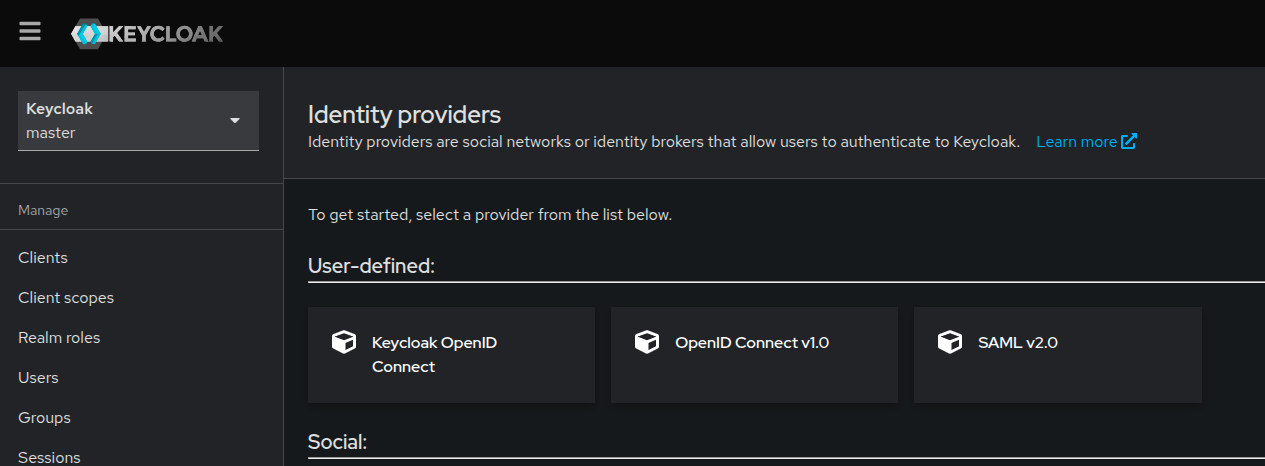
\includegraphics[width=0.9\linewidth]{Bilder/screenshot007}
		\caption{Protokolle für IdPs in Keycloak}
		\label{fig:screenshot007}
	\end{figure}
	
	\vspace{0.5em}
	\textbf{\gls{granttype}n und Authentifizierungsflüsse:}\\
	Keycloak unterstützt verschiedene \textit{Grant Types}, die beschreiben, wie sich Benutzer oder Clients authentifizieren:
	
	\begin{itemize}
		\item \textbf{\gls{authcodegrant}:} Benutzer wird zur Keycloak-Loginseite weitergeleitet. Nach erfolgreicher Authentifizierung erhält der Client einen Authorization Code, den er gegen ein Access Token eintauscht. Das Passwort wird dabei nie an die Client-Anwendung weitergegeben.
		\item \textbf{\gls{clientcredentials}:} Wird für Clients ohne Benutzerinteraktion verwendet. Der Client authentifiziert sich mit seiner Client-ID und einem geheimen Schlüssel (Client Secret), um ein Access Token zu erhalten.
	\end{itemize}
	Die \textbf{Client Authentifizierungsmethode} legt fest, wie der Client gegenüber dem Server seine Identität nachweist – z.\,B. mittels Client Secret oder Zertifikat. Während der Grant-Typ die Art der Anmeldung bestimmt, definiert die Client-Authentifizierungsmethode die technische Form des Identitätsnachweises.
	\\[0.5em]
	Zusätzlich existieren in Keycloak sogenannte \textit{\gls{authflow}s}, die den Ablauf der Authentifizierung steuern:
	
	\begin{itemize}
		\item \textbf{Standard Flow:} Meist Authorization Code Grant mit Weiterleitung zur Login-Seite.
		\item \textbf{Implicit Flow:} Gibt direkt ein Token zurück, wird aber aus Sicherheitsgründen nicht mehr empfohlen.
		\item \textbf{Direct Access Grant:} Direkte Anmeldung über Benutzername und Passwort, z.\,B. bei Skripten oder mobilen Apps.
	\end{itemize}
	
	\begin{figure}[H]
		\centering
		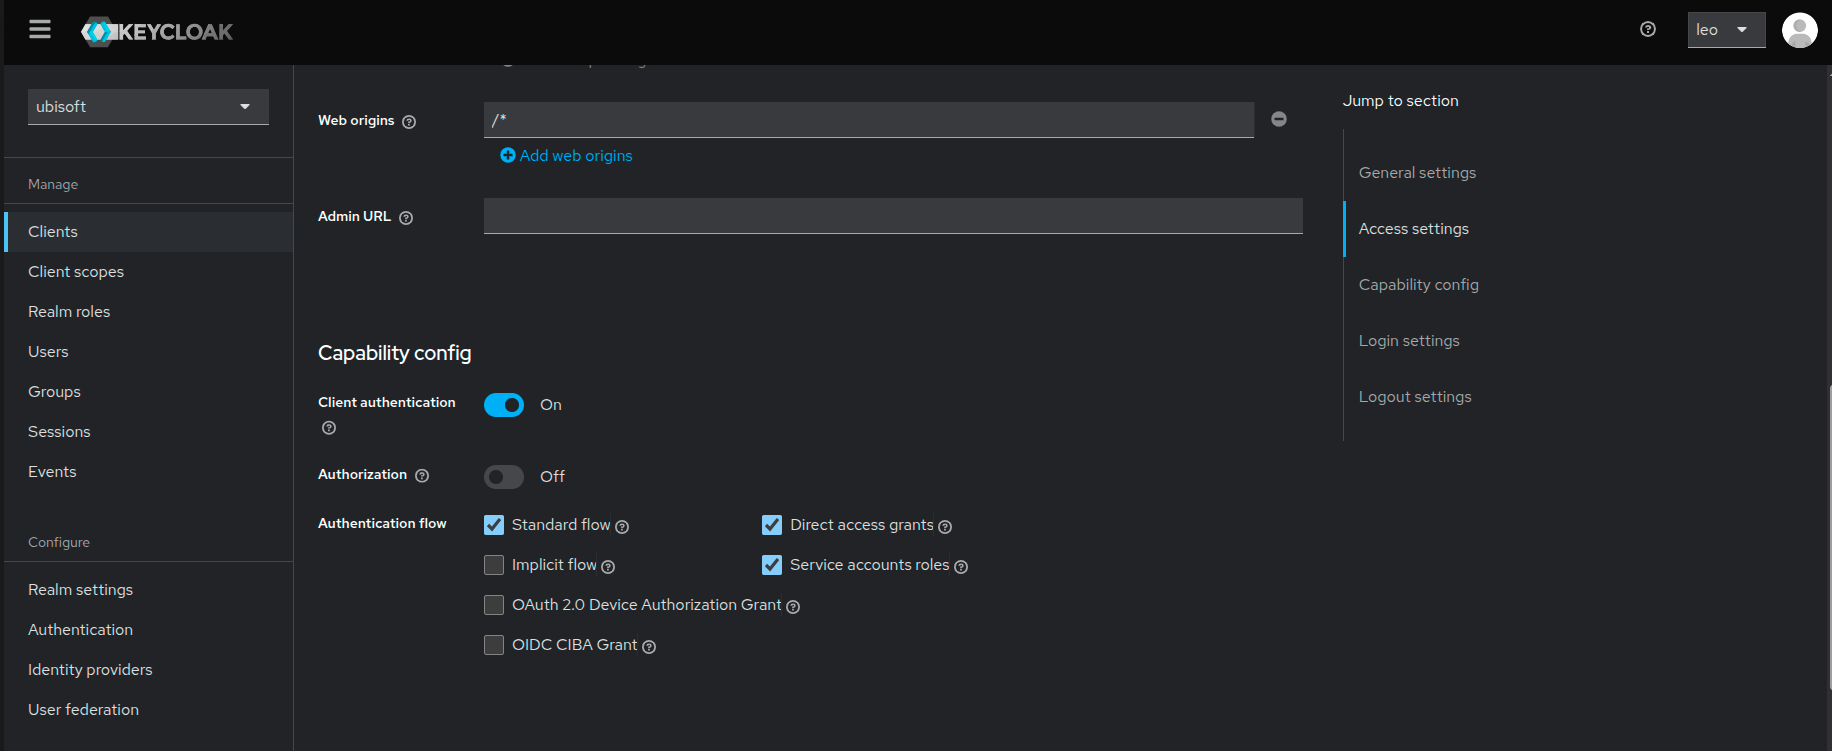
\includegraphics[width=0.9\linewidth]{Bilder/screenshot013}
		\caption{Beispielhafte Konfiguration von Authentication Flows in Keycloak}
		\label{fig:screenshot013}
	\end{figure}
	
	\vspace{0.5em}
	\textbf{\gls{clientscope}:}\\
	Der \textit{Client-Scope} definiert, welche Benutzerdaten in das Token aufgenommen werden, wenn sich ein Benutzer über einen Client anmeldet. Typische Informationen sind Name, Nachname und E-Mail. Diese Daten werden verschlüsselt übertragen, jedoch besteht ein gewisses Risiko bei Missbrauch oder Diebstahl des Tokens.
	
	\vspace{0.5em}
	\textbf{Rollenmodell:}\\
	Keycloak unterscheidet zwei zentrale Rollentypen:
	
	\begin{itemize}
		\item \textbf{Realm-Rollen:} Gelten global innerhalb eines Realms. Sie eignen sich für übergreifende Rechte, z.\,B. „admin“ für alle Clients.
		\item \textbf{Client-Rollen:} Spezifisch für einen einzelnen Client. Sie erlauben feinere Zugriffskontrolle innerhalb der jeweiligen Anwendung.
	\end{itemize}
	
	\vspace{0.5em}
	\textbf{\gls{serviceaccount} Roles:}\\
	Clients können sich in Keycloak auch selbst authentifizieren – ohne Benutzerinteraktion. Wird die \textit{Service Account}-Funktion für einen Client aktiviert, erhält dieser ein eigenes Servicekonto. Dieses Konto kann mit Rollen ausgestattet werden, um Rechte auf bestimmte Ressourcen oder Operationen zu erhalten – z.\,B. für automatisierte Backend-Operationen.
	
	\subsection{Komponenten der Log-Erzeugung}
	Keycloak generiert Logs über verschiedenen Frameworks und Komponenten. Eines davon ist das Logging-Framework von JBoss, wobei moderne Versionen von Keycloak zusätzlich auf das \gls{quarkus}-Framework setzen.
	\vspace{0.5em}
	\textbf{Von \gls{wildfly} zu Quarkus – Technologiewechsel:}\\
	Keycloak basierte in früherer Zeit \textbf{WildFly}-Anwendungsserver\footnote{WildFly Project, \url{https://www.wildfly.org/}, letzter Zugriff: 30. Juli 2025.}
	, der wiederum die \textbf{\gls{jbosslogging}}-Infrastruktur verwendet. Ab der 17. Version von Keycloak wurde WildFly durch das \textbf{Quarkus}-Framework ersetzt. Quarkus unterstützt weiterhin JBoss Logging.
	
	\begin{figure}[H]
		\centering
		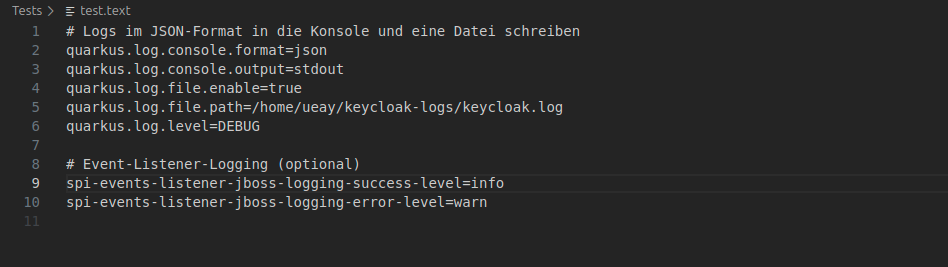
\includegraphics[width=0.9\linewidth]{Bilder/screenshot008}
		\caption{Beispiel: Aktivierung von Quarkus-Logging in der Keycloak-Konfiguration}
		\label{fig:screenshot008}
	\end{figure}
	
	\vspace{0.5em}
	\textbf{Rolle von JBoss Logging:}\\
	JBoss Logging dient in Keycloak als zentrale Logging-API. Es abstrahiert verschiedene Logging-Backends (wie \texttt{\gls{log4j}}, \texttt{JUL}, \texttt{\gls{slf4j}}) und ermöglicht die strukturierte Ausgabe sicherheitsrelevanter Informationen – z.\,B.:
	\begin{itemize}
		\item \texttt{Realm-ID}
		\item \texttt{Benutzer-ID}
		\item \texttt{IP-Adresse}
		\item \texttt{\gls{eventtype}}
	\end{itemize}
	Entwickler müssen sich nicht auf ein spezifisches Logging-Backend festlegen, sondern können über die einheitliche JBoss-API verschiedene Ausgabekanäle konfigurieren (Konsole, Datei, \gls{syslog} etc.).
	
	\vspace{0.5em}
	\textbf{Log4j, Logback oder JUL}\\
	Obwohl es im Java-Ökosystem viele Logging-Frameworks gibt, verzichtet Keycloak bewusst auf deren direkte Verwendung:
	\begin{itemize}
		\item \textbf{Log4j / Logback:} Mächtig, aber externe Abhängigkeiten und teils Sicherheitsrisiken (z.\,B. Log4Shell).
		\item \textbf{JUL (java.util.logging):} Eingebaut, aber funktional begrenzt.
		\item \textbf{Slf4j:} Nur eine Fassade – erfordert Backend wie Logback oder Log4j.
		\item \textbf{\gls{systemout} / System.err:} Nicht strukturiert, ungeeignet für produktive Logs.
	\end{itemize}
	
	\begin{figure}[H]
		\centering
		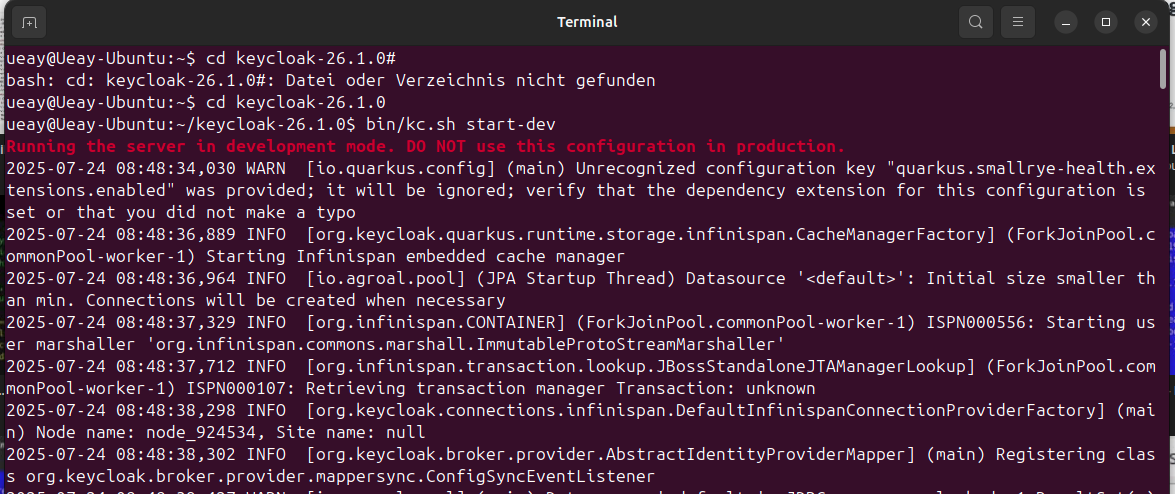
\includegraphics[width=1.1\linewidth]{Bilder/screenshot014}
		\caption{Log-Ausgaben aus einer Quarkus-basierten Keycloak-Instanz}
		\label{fig:screenshot014}
	\end{figure}
	
	\vspace{0.5em}
	Insgesamt stellt JBoss Logging in Kombination mit Quarkus eine erweiterbare Logging-Lösung dar, die sowohl Sicherheitsanforderungen als auch Betriebsanforderungen gerecht wird.
	\vspace{0.5em}
	Ein weiterer Baustein ist SLF4J (Simple Logging Facade for Java), das vor allem in vielen externen Bibliotheken der Java-Welt als Logging-Fassade genutzt wird. Quarkus unterstützt SLF4J indirekt, indem es mit einem passenden Backend wie logback oder log4j2 kombiniert werden kann. In Keycloak selbst wird SLF4J jedoch nicht direkt verwendet, da stattdessen vollständig auf JBoss Logging gesetzt wird.
	\vspace{0.5em}
	Für erweiterte oder spezielle Logging-Anforderungen lassen sich Frameworks wie Log4j2 oder Logback über Custom Extensions oder SPIs einbinden. Diese sind nicht standardmäßig in Keycloak aktiv, können aber in Eigenentwicklungen verwendet werden – etwa wenn besondere Formatierungen oder externe Integrationen erforderlich sind.
	\vspace{0.5em}
	Zudem bietet Keycloak ein eigenes Audit- und Event-Logging-Subsystem, das unabhängig vom allgemeinen Logsystem funktioniert. Mithilfe des EventListener-SPI können verschiedene Ereignisse – etwa Admin-Änderungen oder Benutzeraktionen – gezielt erfasst werden. Die Ausgabe kann dabei in Form einfacher Logs, in Syslog-Formate oder in benutzerdefinierte Kanäle erfolgen.
	\vspace{0.5em}
	Abschließend unterstützt Keycloak die Integration in externe Logging-Systeme durch Syslog oder \gls{remotelogging}. So lassen sich Logs über Tools wie \gls{filebeat} an zentrale Systeme weiterleiten (z.B. Logstash oder Cloud-Dienste wie AWS CloudWatch, Google Stackdriver oder Azure Monitor) oder Kubernetes. Dies ist insbesondere in containerisierten oder skalierenden Cloud-Umgebungen entscheidend für Monitoring, Fehleranalyse und Sicherheitsüberwachung.
	\vspace{0.5em}
	Obwohl Keycloak über ein umfangreiches Logging-Framework auf Basis von JBoss Logging verfügt, das in Kombination mit Quarkus eine zentrale Rolle im Systembetrieb spielt, nutzt diese Arbeit ausschließlich das Event-Logging-Subsystem, welches über die Keycloak-Admin-API zugänglich ist. Die oben beschriebenen Logging-Komponenten dienen damit in erster Linie dem Verständnis der Gesamtarchitektur, sind jedoch nicht direkt Grundlage der durchgeführten Datenanalysen.
	
	\subsection{Log-Dateien in Keycloak}
	Logging, bzw. Protokollierung ist ein essentieller Bestandteil für die Überwachung von IT-Systemen. Für das IT-Monitoring dienen Logs zur Verhinderung und Detektion von Anomalien, sei es im Netzwerk, in einem IoT-Gerät oder eben in IAM-Tools. 
	\\[0.5em]
	Kecyloak unterteilt Logs in folgende Kategorien:
	\begin{itemize}
		\item \gls{serverlogs}: Betriebsstatus, Fehler, Debugging-Infos
		\item \gls{eventlogs}: Benutzer- und Admin-Events (Event-System)
		\item \gls{auditlogs}: Nachvollziehbarkeit von Änderungen (Admin Events)
		\item \gls{accesslogs}: Zugriffsversuche und HTTP-Statuscodes (HTTP Layer / Reverse Proxy)
		\item \gls{securitylogs}: Sicherheitsrelevante Ereignisse und Warnungen
		\item \gls{customlogs}: Erweiterungen und Plugins können eigene Logs erzeugen (SPI)
	\end{itemize}
	Die Logs werden dabei von unterschiedlichen Instanzen in Keycloak erzeugt. Die Server-Logs werden  vom Keycloak-Server selbst erzeugt und weisen die Kategorie \textit{org.keycloak.services} auf. Sie werden mit dem Quarkus-Framework erzeugt.
	\\[0.5em]
	Event-Logs und Audit Logs werden vom Event-System in Keycloak erzeugt, der unter der Kategorie \textit{org.keycloak.events} zu erkennen ist.
	\\[0.5em]
	Access Logs werden auf der Anwendungs- und Netzebene erzeugt- hauptsächlich außerhalb Keycloaks und sind gekennzeichnet als \textit{io.quarkus.http}
	
	\subsection{Event-Logs}
	Analysiert in dieser Arbeit werden die Event-Logs und Admin-Logs. Grund hierfür ist, dass diese wichtige Features enthalten, welche das Benutzerverhalten beschreiben. Server-Logs beziehen sich zu sehr auf Netzbasierte Logs und andere Logs, wie Audit-Logs sind Unterkategorien von Events-Logs. Da keine \gls{spi} verwendet wird und nur die einzelne Keycloak-Instanz untersucht wird, fallen Custom Logs ebenfalls weg als Teil der Trainingsdaten und Security Logs werden nur erzeugt, wenn es die dazu gehörigen Komponenten dazu gibt, welche hier auch nicht angewandt werden.
	\\[0.5em]
	Keycloak unterteilt unter Anderem zwei Arten von Events-Logs:
	
	\begin{itemize}
		\item \gls{adminlogs}(Audit Logs)
		\item \gls{userlogs} (Event Logs)
	\end{itemize}
	Die Admin Logs enthalten alle Logs bzgl. den Operationen des Admins und die User Logs nur die Logs von Benutzern, die nicht Admin sein.
	
	\subsection{Aufbau der Event-Logs}
	Folgende Features sind üblicherweise in den User Event Logs enthalten:
	
	\begin{itemize}
		\item \gls{timestamp}
		\item log\_level
		\item category
		\item type
		\item ipAddress
		\item realmName
		\item realmId
		\item clientId
		\item userId
	\end{itemize}
	Man erkennt, dass wichtige Attribute, wie bspw. der Standort des Clients fehlen. Dies liegt an datenschutzrechtlichen Gründen, jedoch erschwert dies Anomalien in den Logs zu erkennen, weil diese auch anhand eines ungewöhnlichen  Standortes (z.B. Pentagon) erkannt werden. Dies muss noch als Störfaktor genannt werden. Anhand des Standortes können somit schon mal keine Anomalien erkannt werden. Timestamp ist einer der wichtigen Attribute, welche zeigen, zu welchem Zeitpunkt der Log erzeugt wurde. Zur Analyse zeitbasierter Daten eignet sich timestamp als aussagekräftige Information für die LSTM-AE-Hybridmodelle.
	\\[0.5em]
	Des weiteren unterteilt Keycloak noch sogenannte Log-Level. Diese zeigen, ob eine bestimmte Operation erfolgreich war oder nicht oder geben andere Informationen bzgl. einer Operation.
	Bekannte Log-Level sind z.B. INFO, FATAL oder ERROR. Alle Arten finden sich in der Dokumentation \footnote{Keycloak Documentation, „Server Logging“, \url{https://www.keycloak.org/server/logging}, letzter Zugriff: 30. Juli 2025.}.
	Das \gls{loglevel} (z.B. FATAL, ERROR, INFO) bestimmt die Art des Logs, z.B. ob es zum Debugging dient oder eine Warnung erschient, entweder ein Fehler oder eine Info.
	\\[0.5em]
	"\gls{logcategory}" beschreibt hier die Art des Logs.
	\\[0.5em]
	Des weiteren von Bedeutung in den Logs haben die Ereignis-Typen:
	Bspw. ist LOGIN ein Ereignis-Typ bei dem der Benutzer sich anmeldet. Dies wird in Keycloak auch regelmäßig dokumentiert. Andere Ereignistypen sind bspw. \gls{tokenrefresh}, bei dem der Benutzer einen neuen Token bekommt. 
	
	\begin{figure}[H]
		\centering
		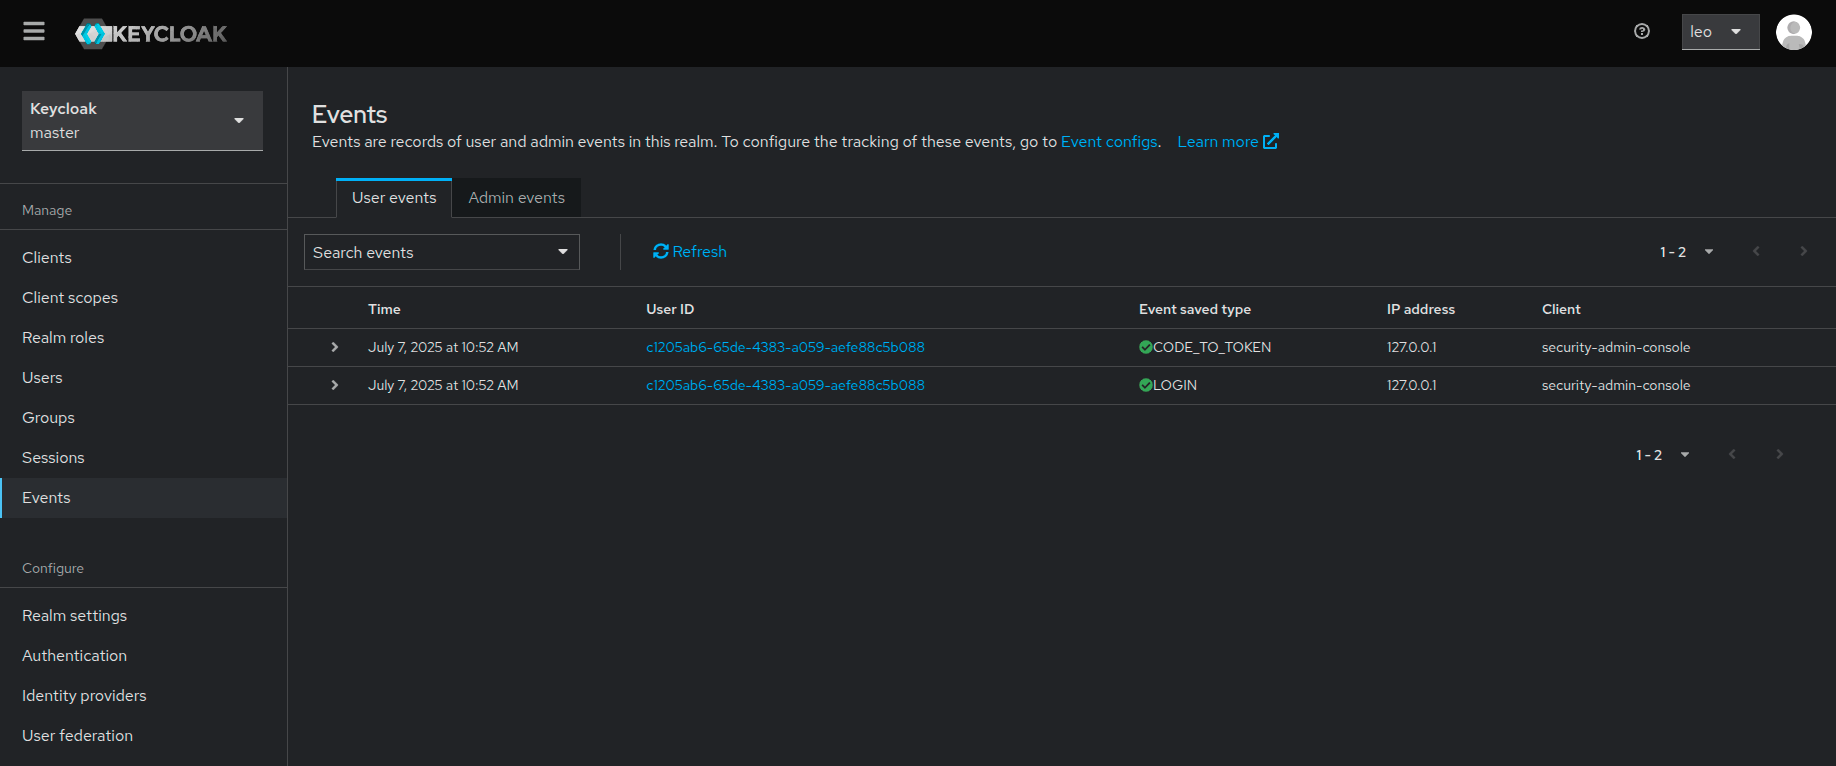
\includegraphics[width=1.0\linewidth]{Bilder/screenshot002}
		\caption{Beispiel Events nach Eventtyp}
		\label{fig:screenshot002}
	\end{figure}
	Je nach Event-Typ werden Features angehängt oder weggelassen, z.B. wird beim Login noch in den Logs die Token-URL, die Art der Verbindung und auch die Art des Authentifizierungsprotokolls angegeben. "Type" steht hier für den Event-Typen. Die wichtigsten Event-Typen sind dabei folgende:
	
	\begin{itemize}
		\item LOGIN: Log, der generiert wird, wenn sich ein Benutzer erfolgreich einloggt über  Keycloak selbst.
		\item \gls{codetotoken}: Wird erzeugt, sobald der Benutzer sich über seine Anmeldedaten auf dem Keycloak-Server authentifiziert hat und von diesem einen Access Token erhalten hat.
		\item \gls{clientlogin}: Log, der generiert wird, sobald sich der Benutzer über einen Drittanbieter einloggt.
		\item \gls{loginerror}: Fehler beim Login über Keycloak
		\item CODE TO TOKEN ERROR: Anmeldedaten war falsch, Server lehnt Anmeldedaten von Benutzer ab
	\end{itemize}
	In den Admin Logs wiederum sind noch Features enthalten, welche in den normalen User Event Logs nicht vorkommen, u.A. '\gls{operationtype}': Diese beinhalten typische CRUD-Operationen wie UPDATE, CREATE, DELETE und ACTION \footnote{Keycloak Community, „JpaAdminEventQuery.java“, GitHub Repository, \url{https://github.com/keycloak/keycloak/blob/main/model/jpa/src/main/java/org/keycloak/events/jpa/JpaAdminEventQuery.java}, letzter Zugriff: 30. Juli 2025.}. 
	
	\section{Theoretischer Hintergrund der Modelle}
	\subsection{LSTM}
	Ein LSTM ist ein spezieller Typ von rekurrentem neuronalen Netzwerk (\gls{rnn}), der entwickelt wurde, um Informationen über längere Zeiträume hinweg zu speichern und verarbeiten \cite{hochreiter1997long}.
	\\[0.5em]
	RNNs gehören zu einer Klasse neuronaler Netzwerke, die sich durch ihre Fähigkeit auszeichnen, sequentielle Daten zu verarbeiten – also Daten, bei denen die Reihenfolge eine zentrale Rolle spielt. Dadurch eignen sie sich insbesondere für die Analyse von Zeitreihen. RNNs speichern frühere Informationen in einem sogenannten \gls{hiddenstate}, der bei jedem Zeitschritt aktualisiert wird. So kann der Kontext vorheriger Eingaben bei der Verarbeitung aktueller Daten berücksichtigt werden.
	\\[0.5em]
	Ein zentrales Problem klassischer RNNs besteht jedoch darin, dass sie bei längeren Sequenzen dazu neigen, frühere Informationen „zu vergessen“. Der Gradient, also der Vektor, welcher anzeigt, in welche "Richtung" sich das Modell verbessern soll, kann beim Zurück-propagieren über viele Zeitschritte hinweg sehr klein werden (sogenannter „Vanishing Gradient“), wodurch der Lerneffekt früherer Daten verloren geht.
	\\[0.5em]
	LSTM-Netzwerke wurden entwickelt, um genau dieses Problem zu lösen \cite[S.19]{staudemeyer2019understanding}. Sie verfügen über eine spezielle Zellstruktur, die es ermöglicht, relevante Informationen über längere Zeiträume hinweg zu speichern. Dies wird durch drei zentrale Steuermechanismen („Gates“) innerhalb der LSTM-Zelle erreicht:
	\begin{itemize}
		\item \textbf{Forget Gate:} Entscheidet, welche Informationen aus dem Zellzustand verworfen werden sollen.
		\item \textbf{Input Gate:} Bestimmt, welche neuen Informationen in den Zellzustand aufgenommen werden.
		\item \textbf{Output Gate:} Regelt, welche Informationen aus dem Zellzustand als Ausgabe weitergegeben werden.
	\end{itemize}
	LSTM-Netzwerke finden in zahlreichen Anwendungsbereichen Verwendung, etwa in der Sprachverarbeitung, bei Vorhersage-Modellen oder im Kontext des Internets der Dinge (IoT) \cite{wei2022lstm}.
	\\[0.5em]
	Die Wahl der Sequenzlänge in einem LSTM beeinflusst maßgeblich die Lern- und Analysefähigkeit. Sehr lange Sequenzen erschweren das Training und können die Erkennung relevanter Muster verringern, da das Modell über viele Zeitschritte hinweg Informationen behalten muss. Kürzere Sequenzen helfen dem Modell, fokussierter auf lokale Muster zu lernen, wodurch sich die Erkennungsgenauigkeit für Anomalien verbessern kann. Eine Herausforderung bei LSTMs ist die Festlegung der passenden Sequenzlänge. Hierarchische multiskalige LSTM-Modelle können dynamisch lernen, auf welchen Zeitskalen Informationen aktualisiert oder zusammengefasst werden sollen, was die flexible Handhabung langer Sequenzen ermöglicht \cite{chung2017hierarchical}.
	Das hierarchisch multiskalige LSTM kann auf verschiedenen Ebenen gleichzeitig lernen, wie weit es „zurückblicken“ oder „zusammenfassen“ muss, um relevante Informationen zu behalten — und so auch sehr lange Sequenzen besser zu verarbeiten. Die Hierarchie sorgt dafür, dass Daten in Ebene gegliedert werden und Multiskalig bedeutet, dass das Modell zeitliche Abhängigkeiten auf mehreren Zeitskalen gleichzeitig betrachtet— also zum Beispiel kurze, mittlere und lange Zeiträume innerhalb der Sequenz.
	\\[0.5em]
	Die Wahl der Sequenzlänge steht oft in engem Zusammenhang mit weiteren Modell- und Trainingsparametern wie der Batch-Größe sowie der Tiefe und Breite des Netzwerks. Eine größere Netzwerktiefe oder -breite kann theoretisch komplexere Muster erkennen, führt aber auch zu höherem Rechenaufwand und größerem Speicherbedarf, was bei langen Sequenzen schnell problematisch wird. Ähnlich kann eine zu große Batch-Größe das Training instabil machen oder den Speicher überfordern, besonders bei tiefen Modellen mit langen Sequenzen. Daher ist das Finden eines guten Gleichgewichts zwischen Sequenzlänge, Netzwerkgröße und Batch-Größe entscheidend, um effizientes Lernen und eine gute Generalisierung zu ermöglichen. Insbesondere bei längeren Sequenzen kann es sinnvoll sein, die Modellkomplexität zu reduzieren oder hierarchisch-multiskalige Architekturen zu nutzen, um die Verarbeitung effizienter zu gestalten \cite{bengio1994learning}.
	\\[0.5em]
	Da aber in dieser Arbeit nicht mit Millionen von Dateneinträgen gearbeitet wird, liegt der Fokus darauf, die Sequenzlänge gering zu halten, weil LSTMs darin scheitern, korrektes Zählverhalten auf deutlich längeren Sequenzen zu generalisieren, selbst wenn sie dies auf kürzeren Sequenzen während des Trainings scheinbar gelernt haben. \cite{elnaggar2022counting}.
	
	\subsection{Autoencoder}
	Ein Autoencoder ist ein spezieller Typ neuronalen Netzwerks, das aus zwei Hauptkomponenten besteht: einer \gls{encoder}- und einer \gls{decoder}-Schicht \cite[S.3]{michelucci2022introduction}.
	\\[0.5em]
	Die Encoder-Schicht komprimiert die Eingabedaten, indem sie deren Dimension reduziert und sie auf eine kompakte Repräsentation abbildet – die sogenannte \gls{bottleneck}-Schicht. Diese Engstelle zwingt das Modell dazu, die wesentlichen Merkmale der Daten in verdichteter Form zu erfassen. Dabei werden redundante oder irrelevante Informationen herausgefiltert, was es dem Autoencoder ermöglicht, die „Essenz“ der Daten zu lernen.
	\\[0.5em]
	Die Decoder-Schicht nimmt diese komprimierte Repräsentation und rekonstruiert daraus die ursprünglichen Eingabedaten. Das Ziel des Netzwerks ist es, durch Minimierung des \gls{rekonstruktionsfehler}s – also der Differenz zwischen Eingabe und Ausgabe – eine möglichst originalgetreue Rekonstruktion zu erreichen. Der Rekonstruktionsfehler ist auch in der später vorgestellten Hybridarchitektur von zentraler Bedeutung.
	\\[0.5em]
	Durch diese Eigenschaften eignen sich Autoencoder besonders gut für Aufgaben wie die Anomalieerkennung. Weicht eine Eingabe signifikant von den zuvor gelernten Mustern ab, gelingt die Rekonstruktion schlechter – der Rekonstruktionsfehler steigt. Dies kann als Indikator für potenzielle Anomalien genutzt werden.
	
	\paragraph{Bottleneck und seine Bedeutung}
	Der Bottleneck ist entscheidend, da er die Kapazität des Autoencoders steuert. Ein zu kleiner Bottleneck kann dazu führen, dass wichtige Informationen verloren gehen und die Rekonstruktion schlecht wird. Ein zu großer Bottleneck hingegen erlaubt es dem Netzwerk, einfach Daten "durchzuschleusen". Um zu verhindern, dass das Modell im Bottleneck redundante Merkmale lernt, wird die Verlustfunktion erweitert. Dadurch wird das Netzwerk dazu angeleitet, möglichst vielfältige und wenig überlappende Merkmale zu lernen \cite{laakom2022reducing}.
	
	\paragraph{Varianten und Architekturen}
	Neben dem klassischen Autoencoder gibt es weitere Varianten, z.B. den \gls{vae} (VAE), der probabilistische Modelle nutzt und generative Fähigkeiten besitzt, oder den \gls{denoising}, der lernt, verrauschte Eingaben zu bereinigen. Außerdem können Autoencoder aus mehreren Schichten bestehen (deep Autoencoder), um komplexere Merkmale zu extrahieren. Da für diese Arbeit keine zu großen, aufwendigen Daten erstmals analysiert werden können, aufgrund mangelnder Trainingsdaten- wird ein Deep Autoencoder auch nicht zum Einsatz kommen.
	
	\paragraph{Anwendungsbereiche}
	Autoencoder finden Anwendung in der Bildkompression, Anomalieerkennung in Netzwerken oder Produktionsprozessen, Feature Learning vor Klassifikationsaufgaben oder generativer Modellierung. 
	
	\begin{figure}[H]
		\centering
		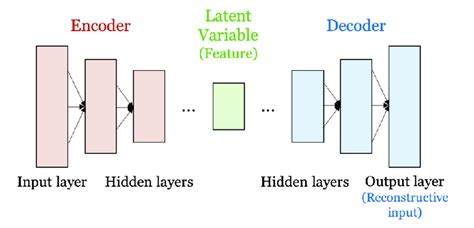
\includegraphics[width=0.7\linewidth]{Bilder/screenshot004}
		\caption{Visuelle Darstellung der Funktion des AEs, Quelle: https://www.researchgate.net/figure/Structure-of-the-autoencoder\_fig1\_365074431, Letzter Zugriff am: 15.07.2025}
		\label{fig:screenshot004}
	\end{figure}
	
	\paragraph{Mit dem LSTM kombiniert}
	Autoencoder lassen sich besonders gut mit Long Short-Term Memory (LSTM)-Netzwerken kombinieren, wenn es um sequenzielle oder zeitabhängige Daten geht. Während der klassische Autoencoder oft für statische Daten verwendet wird, können LSTM-Autoencoder zeitliche Abhängigkeiten erfassen und lernen, wie sich Daten über Zeit entwickeln.
	\\[0.5em]
	Ein LSTM-Autoencoder nutzt LSTM-Zellen im Encoder und Decoder, um komplexe zeitliche Muster zu erfassen und zu rekonstruieren. Diese Kombination ist besonders nützlich bei Anomalieerkennung in Zeitreihen, wie etwa in der Überwachung von Maschinenzuständen, Finanzdaten oder Netzwerksicherheit. Anomalien fallen hier oft durch signifikant erhöhte Rekonstruktionsfehler auf, da die zeitlichen Muster nicht gut rekonstruiert werden können.
	\\[0.5em]
	Durch die Fähigkeit von LSTM, langfristige Abhängigkeiten zu modellieren, und die Komprimierung des Autoencoders entsteht ein mächtiges Werkzeug für die Analyse und das Verständnis komplexer, sequenzieller Daten.
	
	\subsection{Isolation Forest}
	Isolation Forest ist ein unüberwachter Lernalgorithmus, welcher durch Partitionen Daten voneinander trennen kann, indem er binäre Bäume erzeugt. Er unterteilt die Daten so lange, bis keine Isolierung der Daten mehr möglich ist. Durch dieses Vorgehen lasen sich auch Anomalien erkennen: Die Anomalien werden je danach erkannt, wie isoliert die Daten eingeteilt wurden. Je isolierter die Datenpunkte aufgeteilt wurden, desto wahrscheinlicher ist es, dass es eine Anomalie ist. Wenn sich Datenpunkte in ihrer Form ähneln, so würde der Algorithmus diese nicht zu stark isolieren. Lassen sich diese jedoch stark anhand ihrer Merkmale isolieren, so  ist es wahrscheinlicher, dass diese keiner üblichen Menge eingeteilt werden kann. Isolation Forest ist im Vergleich zu anderen Algorithmen recht gut für hoch-dimensionale Daten geeignet \cite{liu2008isolation}.
	\\[0.5em]
	\begin{figure}
		\centering
		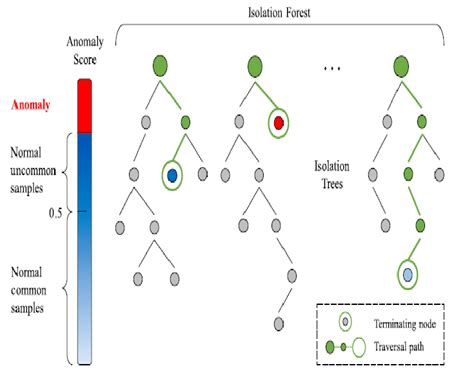
\includegraphics[width=0.7\linewidth]{Bilder/screenshot005}
		\caption{Visuelle Darstellung der Funktion des AEs, Quelle: https://www.researchgate.net/figure/Anomaly-Detection-using-Isolation-Forest-18\_fig3\_350551253, Letzter Zugriff am: 15.07.2025}
		\label{fig:screenshot005}
	\end{figure}
	Der Algorithmus erzeugt \gls{isolationtree}s, welche aus Blattknoten oder aus einem inneren Knoten besteht,der eine Testregel enthält, die die Daten in zwei Gruppen aufteilt. Die Testregel besteht aus einem Wert aus der Auswahl eines Merkmals  q und einem Schwellenwert p, so dass alle Datenpunkte, deren Wert für q kleiner als p ist, in den linken Kindknoten kommen, und alle anderen in den rechten Kindknoten.
	\\[0.5em]
	Zum Aufbau eines solchen Baums nimmt man eine Stichprobe von Datenpunkten und teilt sie rekursiv auf, indem man zufällig ein Merkmal und einen Split-Wert auswählt. Dieser Prozess wird so lange wiederholt, bis
	eine maximale Baumhöhe erreicht ist, nur noch ein Datenpunkt übrig ist, oder
	alle Datenpunkte im aktuellen Teilbaum identisch sind \cite[S.3]{liu2008isolation}.
	\\[0.5em]
	Das Ergebnis ist ein vollständiger binärer Baum, bei dem jeder Datenpunkt in einem Blattknoten isoliert wird.
	\\[0.5em]
	Wenn alle Datenpunkte unterschiedlich sind, dann gilt:
	\begin{itemize}
	\item Es gibt genauso viele Blätter wie Datenpunkte (n).
	
	\item Die Anzahl der inneren Knoten ist n - 1.
	
	\item Insgesamt hat der Baum 2n - 1 Knoten.
	
	\item Der Speicherbedarf wächst also linear mit der Anzahl der Datenpunkte.
	\end{itemize}
	Isolation Forest unterteilt jedoch zufällig die Datenpunkte, wobei man die Sinnhaftigkeit des Algorithmus hinterfragen kann.
	
	\subsection{One-Class SVM}
	Da viele Angriffe durch die Analyse von System-Logdaten erkennbar sind, wurde ein Ansatz entwickelt, der auf One-Class Support Vector Machines (OC-SVM) basiert und mit abstrahierten Benutzeraudit-Logs aus dem DARPA-Datensatz von 1999 trainiert wurde \cite{li2003improving}. Die Methode nutzt eine nichtlineare Abbildung der Daten in einen höherdimensionalen Raum, um auch nichtlinear trennbare Daten linear trennbar zu machen:
	„Bei nichtlinear trennbaren Daten können wir sie durch eine nichtlineare Abbildung in einen hochdimensionalen Raum transformieren, so dass die Datenpunkte linear trennbar sind.“
	\\[0.5em]
	\begin{figure}
		\centering
		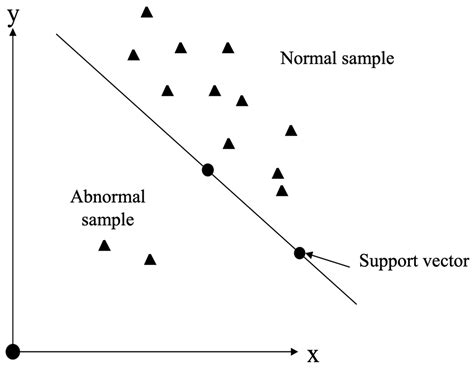
\includegraphics[width=0.7\linewidth]{Bilder/screenshot006}
		\caption{Visuelle Darstellung  OCSVM. Quelle: https://www.mdpi.com/2076-3417/13/3/1734, Letzter Zugriff am: 15.07.2025}
		\label{fig:screenshot006}
	\end{figure}
	Ein zentrales Problem bei One-Class Support Vector Machines (\gls{ocsvm}) besteht darin, dass der Ursprung im \gls{feature-space} als Repräsentant für Anomalien dient, obwohl dies in der Realität nicht immer zutrifft \cite{bounsiar2025oneclass}. In ihrer Arbeit erklären die Autoren, dass die Trennung der Zielklasse vom Ursprung (also von den Ausreißern) häufig missverstanden wird. Sie schlagen eine geometrische Interpretation vor, bei der die Zielklasse vom übrigen Raum getrennt wird, insbesondere wenn ein Gauß-Kernel verwendet wird.
	
	\subsection{DBSCAN}
	DBSCAN ist ein dichtebasiertes Cluteringverfahren, dass Datenpunkte anhand ihrer Dichte zu anderen Punkten klassifizieren kann.
	Die Dichte wird durch die Anzahl der Nachbarpunkte innerhalb eines Radius (Eps) gemessen, wobei mindestens eine Mindestanzahl von Punkten (MinPts) in diesem Radius vorhanden sein muss \cite{ester1996dbscan}. Die Wahl dieser Parameter ist entscheidend für den Erfolg der Klassifizierung.
	
	\begin{figure}[H]
		\centering
		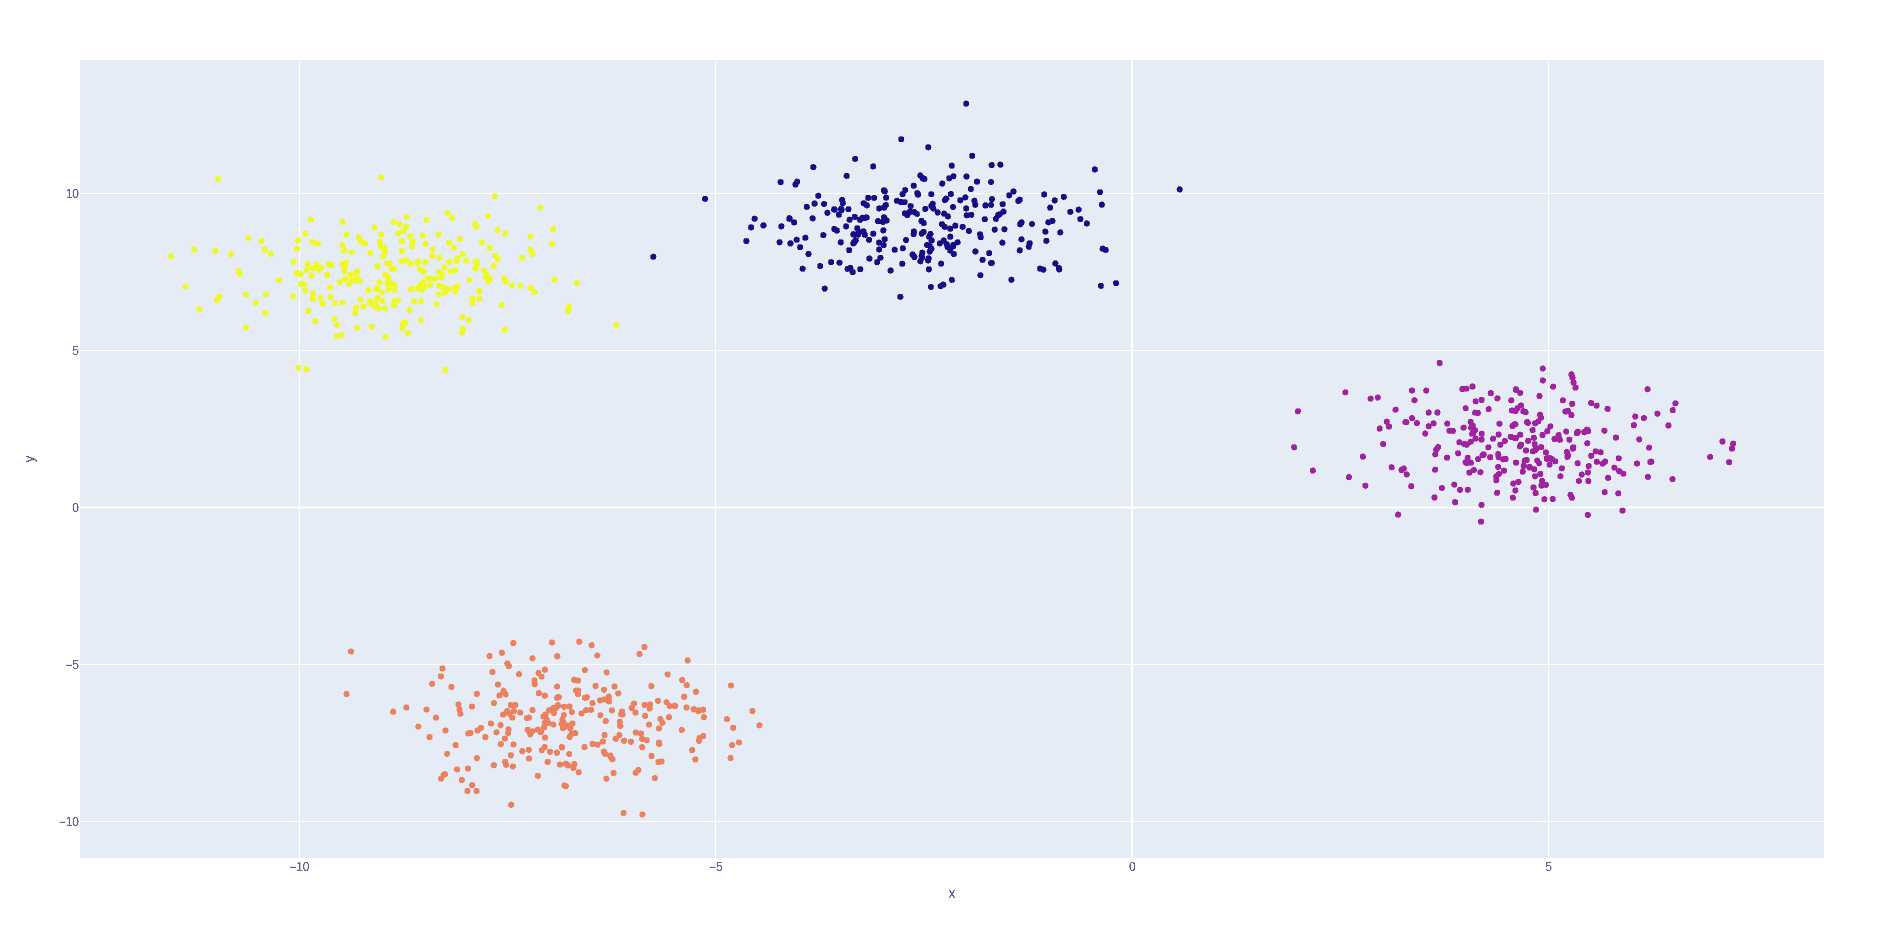
\includegraphics[width=0.9\linewidth]{Bilder/screenshot015}
		\caption{Beispiel DBSCAN-Cluster, Quelle: \url{https://www.baeldung.com/wp-content/uploads/sites/4/2023/04/clusters.png}, Letzter Zugriff am: 15.07.2025}
		\label{fig:screenshot015}
	\end{figure}
	Der Algorithmus läuft folgendermaßen ab:
	Man startet von einem bestimmten Punkt p. Daraufhin werden alle Punkte gesucht, welche sich in der Nähe von p befinden. Sobald eine Mindestanzahl von \textit{Eps} erreicht ist, die auch durch \textit{MinPts} festgelegt wird, so bildet sich ein Cluster. Danach werden alle Punkte die nun zu einem Cluster gehören, aus einer Liste an verbleibenden Punkten herausgenommen. Daraufhin wird p zufällig an einen weiteren Ort im Raum platziert, wo noch kein Cluster gebildet wurde. Dies geschieht solange, bis keine Punkte in der Liste übrig sind.Eine hohe Anzahl von \gls{noise}-Punkten kann darauf hinweisen, dass die Klassifikation nicht optimal gelungen ist \cite{ester1996dbscan}. 
	
	\subsection{Alternative Algorithmen}
	Es wurde als Alternative zu DBSCAN auch das hierarchische Verfahren \gls{hdbscan} (Hierarchical Density-Based Spatial Clustering of Applications with Noise) in Betracht gezogen. HDBSCAN ist in vielerlei Hinsicht robuster als DBSCAN,  insbesondere bei der Identifikation von Clustern in hochdimensionalen oder verrauschten Daten \cite{campello2015hierarchical}. Ein Vorteil von HDBSCAN ist, dass es keine globale Dichte-Schwelle benötigt und sich besser an lokale Datenstrukturen anpasst. Aufgrund der derzeit noch begrenzten Anzahl an Studien und praktischen Erfahrungswerten zu HDBSCAN im konkreten Anwendungsbereich wurde jedoch auf den Einsatz verzichtet. Für zukünftige Arbeiten wäre es durchaus interessant, HDBSCAN in Kombination mit LSTM-AE näher zu untersuchen.
	\\[0.5em]
	Darüber hinaus wurden auch weitere Anomalieerkennungsverfahren wie \gls{kmeans} und \gls{lof} (Local Outlier Factor) evaluiert. K-Means wird sogar als effektivster Algorithmus dargestellt im Vergleich zu anderen \cite{vinces2025comparative}.
	\\[0.5em]
	LOF erkennt Ausreißer, indem es die lokale Dichte eines Datenpunkts mit der seiner Nachbarn vergleicht und Punkte mit stark abweichender Dichte als potenzielle Anomalien markiert- es ist auch wissenschaftlich bewiesen, dass er sich gut zur Erkennung von Anomalien eignet \cite{breunig2000lof}.
	\\[0.5em]
	Kurz gefasst: Beide Verfahren eignen sich sehr gut zur Erkennung von Anomalien und wurden daher ebenfalls berücksichtigt. Einer Studie zufolge ist OCSVM in Bezug auf die Anomalie-Erkennung jedoch überlegen \cite{budiarto2025unsupervised}. Zudem leidet auch LOF unter dem „Fluch der Dimensionalität“, da es auf Dichte-Schätzungen im euklidischen Raum (z. B. k-Nächste-Nachbarn-Distanzen) basiert, welche in hochdimensionalen Räumen an Aussagekraft verlieren. Dieses Problem ist bekannt und wird in der Literatur mehrfach beschrieben \cite[S.366]{zimek2012survey}. Die Frage, warum dennoch DBSCAN zusammen mit OCSVM und Isolation Forest gewählt wurde, obwohl diese ebenfalls betroffen sind, lässt sich mit einer Begrenzung des Arbeitsumfangs erklären. Darüber hinaus ähneln sich einige der ausgewählten Algorithmen denen, die nicht gewählt wurden: So ist K-Means beispielsweise ein Clustering-Algorithmus, ähnlich wie DBSCAN, und LOF weist Parallelen zum Isolation Forest auf. 
	\\[0.5em]
	Um eine möglichst hohe Varianz und einen ausgewogenen Vergleich zu gewährleisten, wurden daher sich ähnelnde Algorithmen bewusst ausgeschlossen.
	Ein weiterer Grund- mitunter der Hauptgrund- weshalb beide abgelehnt wurden war die Tatsache, dass K-Means (ohne Optimierungsmechanismen) bei zu großen Datensätzen Skalierungsprobleme hat und dass LOF (ohne Optimierungsmechanismen), ebenfalls bei zu großen Datensätzen einen hohe Rechenzeit hat \cite{mussabayev2023kmeans,springerlof2023}.
	
	\section{Implementierung}
	\subsection{Hybridmodelle mit LSTM-AE}
	Generell wurden die Modelle nach der selben Architektur gebaut:
	
	\begin{figure}[H]
		\centering
		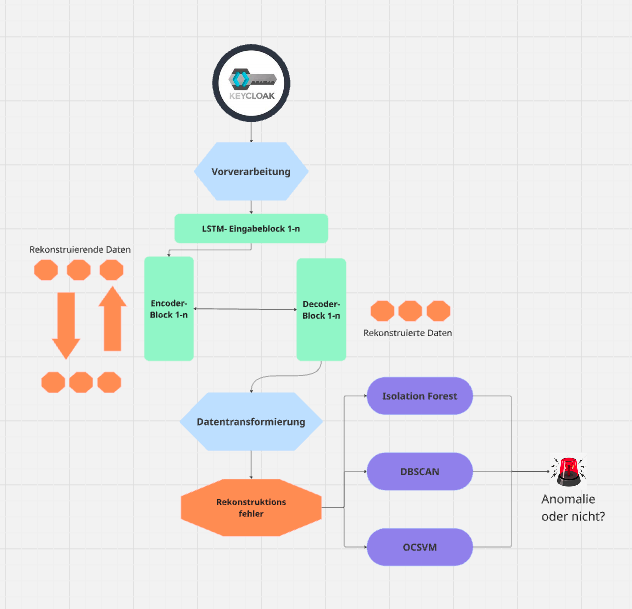
\includegraphics[width=0.9\linewidth]{Bilder/screenshot001}
		\caption{Skizze aller Hybridmodelle}
		\label{fig:screenshot001}
	\end{figure}
	
	man entschied sich für folgende Parameter:
	\begin{table}[h]
		\centering
		\begin{tabular}{ll}
			\toprule
			\textbf{Parameter}       & \textbf{Wert}            \\
			\midrule
			batch\_size             & 32                      \\
			dropout\_rate            & 0.1                      \\
			encoder\_layers         & [128, 64]         \\
			decoder\_layers         & [64, 128]         \\
			learning\_rate          & 0.001                   \\
			\bottomrule
		\end{tabular}
		\caption{Bestimmte Parameter der Modellkonfiguration}
		\label{tab:model_params}
	\end{table}
	Man entschied sich für eine Architektur mit zwei Schichten im Encoder und Decoder (Tiefe) sowie 128 (Breite), um einen ausgewogenen Kompromiss zwischen Informationsreduktion zu erzielen.
	Diese Dimensionierung ermöglicht es dem Modell, komplexe zeitliche Muster in den Daten ausreichend zu komprimieren, ohne wesentliche Strukturen zu verlieren. Eine geringere Breite hätte hingegen das Risiko erhöht, dass relevante Informationen verloren gehen. Es muss schon hier erwähnt werden, dass die Reliabilität dieser Arbeit durch die Regularisierungstechniken beeinflusst wird, was aber notwendig ist, da dies übliche Techniken sind, um Overfittung zu vermeiden.
	\\[0.5em]
	Zudem wird die sogenannte Dropoutrate eingesetzt, eine Regularisierungstechnik, die Overfitting verhindert. Dabei werden während des Trainings zufällig einzelne Neuronen deaktiviert. Die Dropoutrate wurde relativ gering gewählt, um die Testläufe nicht zu stark zu randomisieren und die Reliabilität der Ergebnisse zu verbessern. Aufgrund der durch diese Technik entstehenden Schwankungen ist es wichtig, beim Training und Testen der Modelle mehrere Läufe durchzuführen, um die Verteilung der Ergebnisse zu analysieren und Unterschiede zu erkennen.
	\\[0.5em]
	Die Daten werden zuerst in numerische Daten umgewandelt- wenn sie noch nicht numerisch sind. Absichtlich werden NaN-Werte und unklare Werte nicht bereinigt, sondern in eine eigene Kategorie gefasst, die auch ins numerische umgewandelt wird. Dies ist wichtig, da auch solche Werte Anomalien darstellen und die Bereinigung dieser Daten dafür sorgen würde, dass potenzielle Gefahrenquellen unerkannt bleiben. NaN-Werte können außerdem bspw. bei falschen Accounts oder vielleicht bei Bots auftreten, weshalb es wichtig ist, diese in der Analyse beizubehalten. Die numerischen Daten werden durch den LabelEncoder \footnote{https://scikit-learn.org/stable/modules/generated/sklearn.preprocessing.LabelEncoder.html} erzeugt. Die Daten werden danach skaliert mit dem StandardScaler \footnote{https://scikit-learn.org/stable/modules/generated/sklearn.preprocessing.StandardScaler.html}.
	\\[0.5em]
	Der LSTM-AE wird dabei nur auf normalen Daten trainiert. Dies liegt an der Natur des Autoencoders- denn dieser rekonstruiert Daten nur wieder. Wenn er lange genug trainiert wird, "lernt" er nur "normale" Daten zu konstruieren. In Testdaten, wo sich dann die Anomalien befinden, kann er schlechter rekonstruieren. Daraus entsteht dann der sogenannte Rekonstruktionsfehler.
	\\[0.5em]
	\begin{figure}[H]
		\centering
		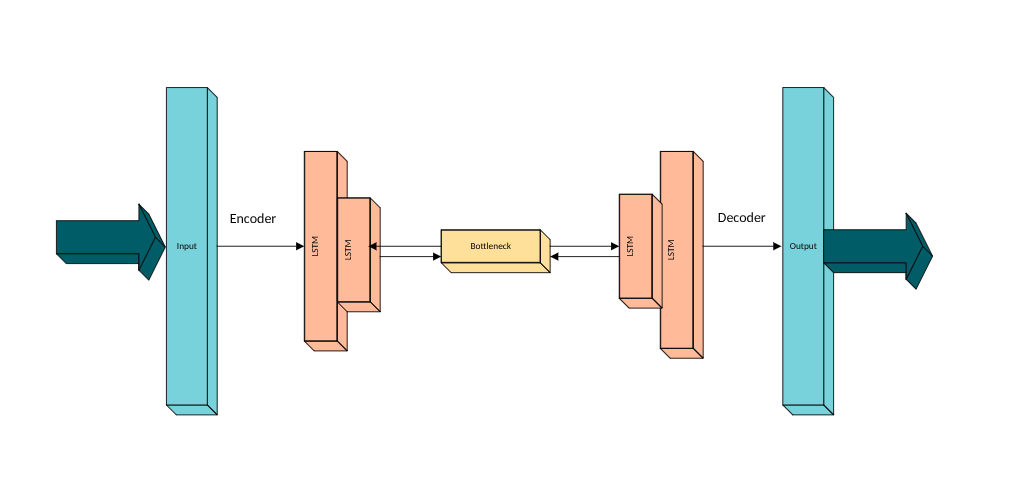
\includegraphics[width=1.2\linewidth]{Bilder/screenshot-lstm}
		\caption{Gesamtarchitektur LSTM-AE}
		\label{fig:screenshot-lstm}
	\end{figure}
	Dieser Trainingsfehler, bzw. Rekonstruktionsfehler, also die Daten, welche nicht klar klassifiziert werden konnten, werden danach jeweils mit einem der Anomalieerkennungs-Algorithmen(IF, OCSVM, DBSCAN) trainiert. Dies ist auch eine Vorangehensweise, welche bspw. in der Studie von Malhotra bekannt ist \cite{malhotra2016lstm}.
	\\[0.5em]
	Dadurch kann jedes Modell separat trainiert, getestet und evaluiert werden, was eine modulare Struktur gewährleistet, auch wenn die gesamte Umsetzung in einem Jupyter Notebook erfolgt.
	\\[0.5em]
	Die Sequenzlänge wird gering gehalten, um nicht zu viele Daten zu generieren, da eine zu hohe Sequenzlänge kontraproduktiv ist. Auch die Batch-Size wird gering gehalten, damit sie mit der Sequenzlänge harmoniert. Die Sequenzlänge gibt an, wie viele Logs gleichzeitig analysiert werden und deren Zusammenhänge erkannt werden. Die Batch-Size gibt an, wie groß die Eingabe dieser Sequenzen sein darf (weshalb sie proportional zueinander sein müssen). Für die Sequenzlängen wird in den letzten Abschnitten Testfälle angewandt.
	
	
	\paragraph{Encoder-Decoder Struktur und Bidirektionales LSTM}  
	Die Architektur folgt dem Prinzip eines Encoder-Decoder-Systems, bei dem der Encoder die Aufgabe übernimmt, die wesentlichen Merkmale der Eingabesequenzen in einem kompakten, latenten Raum zu repräsentieren. Dieser latente Raum fasst die zeitlichen Muster und Strukturen zusammen, wodurch eine effizientere Repräsentation ermöglicht wird. Das bidirektionale LSTM im Encoder erlaubt es, Informationen nicht nur aus der Vergangenheit, sondern auch aus der Zukunft innerhalb der Sequenz zu erfassen, was besonders bei zeitlich stark korrelierten Daten von Vorteil ist. Der Decoder hingegen nutzt diese latente Repräsentation, um die ursprüngliche Sequenz zu rekonstruieren, wodurch eine präzise Nachbildung der Eingabedaten sichergestellt wird.
	
	\paragraph{Verlustfunktion und Optimierung}  
	Zur Bewertung der Modellgüte wird die mittlere quadratische Abweichung (\textit{Mean Squared Error}, MSE \footnote{https://scikit-learn.org/stable/modules/generated/sklearn.metrics.mean\_squared\_error.html}) herangezogen, welche die Differenz zwischen Eingabe- und Ausgabesequenzen quantifiziert. MSE eignet sich zur Messung der Rekonstruktionsqualität bei kontinuierlichen Werten, da größere Fehler durch die Quadratisierung stärker gewichtet werden, was eine präzise Anpassung des Modells erzwingt. Die Optimierung erfolgt mittels des Adam-Optimierers \footnote{https://docs.pytorch.org/docs/stable/generated/torch.optim.Adam.html}, welcher durch Lernraten für jeden Parameter besticht und somit eine schnelle und stabile Konvergenz auch bei komplexen Modellen gewährleistet. Die Lernrate stellt dabei einen wesentlichen Hyperparameter dar, der das Tempo der Gewichtsaktualisierungen steuert und einen Balanceakt zwischen schnellem Lernen und stabiler Anpassung darstellt.
	
	\paragraph{Berechnung des Rekonstruktionsfehlers}
	Die Idee, durch den Mean Square Error den Rekonstruktionsfehler zu berechnen stammt von Torabi et Al. \cite[S. 5]{torabi2023practical}. Die allgemein Formel zur Berechnung des Fehlers lautet wie folgt:
	
	\[
	\text{Reconstruction Error} = \frac{1}{T \cdot F} \sum_{t=1}^{T} \sum_{f=1}^{F} \left( x_{t,f} - \hat{x}_{t,f} \right)^2
	\]
	Im Grunde genommen wird hier jeder Fehler als Zeitpunkt dargestellt. Jeder Zeitpunkt (I) und jedes Feature F stellt hier eine Abhängigkeit dar. Alle rekonstruierbaren Werte werden von den nicht-rekonstruierbaren über jedes Logs hinweg berechnet – und anschließend der Durchschnitt berechnet wird. Dies ist dann der gesamte Rekonstruktionsfehler.
	
	\paragraph{Ermittlung des Schwellenwertes}
	Ab wann soll das Modell eine Anomalie erkennen? Soll es schon bei einer kleinen Abweichung eines Features es als Anomalie deuten oder erst ab großen Unterschieden? Jablonski et Al. \cite{jablonski2023automatic} haben dies untersucht und sind zu folgendem Algorithmus gekommen:
	Man extrahiert einfach alle Rekonstruktionsfehler aus den Daten und sortiert sie zuerst. Der optimale Schwellenwert ist genau die Mitte zwischen zwei Werten, wo der größte Abstand im sortierten Fehlervektor gefunden wurde.
	Nach den Autoren sei dies ein optimaler Weg, um den Schwellenwert zu erkennen. Dieser wurde jedoch in dieser Arbeit später verworfen, weil man mit diesem Ansatz schlechtere Ergebnisse in Precision und Recall für alle Hybridmodelle erhielt. Ursache dafür ist wahrscheinlich, dass die Anomalien im verhältnis zu Anzahl normaler Logs zu gering ist. Um Anomalien in Zeitreihen zuverlässig zu erkennen, ist es notwendig, die Rohwerte der Anomalie-Score-Funktion (die Rekonstruktionsfehler, die von Modellen wie Isolation Forest oder OCSVM berechnet werden) in binäre Entscheidungen zu übersetzen. Hierzu wird ein Threshold festgelegt: Werte oberhalb des Thresholds werden als Anomalien klassifiziert, Werte darunter als normal. Die Wahl des Thresholds hat direkten Einfluss auf die Balance zwischen Precision (wie viele als Anomalien erkannten Punkte tatsächlich Anomalien sind) und Recall (wie viele der echten Anomalien erkannt werden). Um diese Balance optimal zu berücksichtigen, verwenden wir den F1-Score, der Precision und Recall kombiniert. Der Threshold wird so gewählt, dass der F1-Score maximiert wird. Dieser Ansatz erwies sich als effektiver und es ist auch bewiesen, dass dies ein guter Ansatz ist, um den Schwellenwert zu berechnen, auch besonders bei Halb-Überwachten Lernmodellen \cite{wilkinghoff2024f1ev}.
	
	\subsubsection{Implementierung: Isolation Forest}
	Im Fall des Isolation Forest wird ein auf Entscheidungsbäumen basierender Algorithmus genutzt, der speziell für die Erkennung von Ausreißern in hochdimensionalen Daten entwickelt wurde. Das Modell wird auf den Fehlerwerten der Trainingsdaten trainiert und anschließend auf die Testdaten angewendet.
	Anstatt die standardmäßige Vorhersage (-1 = anomal, 1 = normal) direkt zu verwenden, werden die Rohscores des Modells herangezogen, um mittels einer F1-basierten Schwellenwert-Optimierung eine binäre Klassifikation zu erzeugen. Hierbei wird für jede Sequenz ein optimaler Schwellenwert ermittelt, der die F1-Metrik maximiert. Alle Punkte mit Scores oberhalb dieses Schwellenwerts werden als Anomalien (1) klassifiziert, alle anderen als normal (0).
	Da die Daten sequenzbasiert aufgebaut sind – beispielsweise aus Zeitreihen bestehen – erfolgt eine Anpassung der Labels: Aus den Zielwerten der Testdaten wird jeweils das Label der letzten Position jeder Sequenz extrahiert, sodass ein Vergleich zwischen den binären Vorhersagen und den tatsächlichen Labels möglich ist.
	
	\subsubsection{Implementierung: OCSVM}
	Für die Umsetzung der One-Class SVM wird das Modell mit einem \gls{nu}-Wert initialisiert, der die erwartete Obergrenze an Ausreißern im Trainingsdatensatz festlegt. Zusätzlich wird kein \gls{gamma}-Parameter gesetzt, sodass der RBF-Kernel automatisch die Standard-Einstellung (gamma='scale') verwendet.
	Anstatt die Standardvorhersage (-1 = anomal, 1 = normal) direkt zu verwenden, werden die Rohscores der Entscheidungsfunktion genutzt, um mittels einer F1-basierten Schwellenwert-Optimierung eine binäre Klassifikation zu erzeugen. Hierbei wird für jede Sequenz ein optimaler Schwellenwert ermittelt, der die F1-Metrik maximiert. Punkte oberhalb dieses Schwellenwerts werden als Anomalien (1) klassifiziert, die übrigen als normal (0).
	Da die Daten sequenzbasiert aufgebaut sind – beispielsweise aus Zeitreihen bestehen – wird aus den Testlabels jeweils das Label der letzten Position jeder Sequenz extrahiert, um die binären Vorhersagen korrekt mit den tatsächlichen Labels vergleichen zu können.
	
	\subsubsection{Implementierung: DBSCAN}
	Das DBSCAN-Modell wird direkt auf die Rekonstruktionsfehler der Testdaten angewendet. Dabei werden keine festen Werte für \texttt{eps} und \texttt{min\_samples} vorgegeben, sodass das Modell flexibel auf die vorliegenden Daten reagieren kann. Die Methode \texttt{fit\_predict()} liefert für jeden Punkt entweder eine Clusterzuweisung (0, 1, …) oder -1, wobei -1 Datenpunkte kennzeichnet, die als Rauschen bzw. Anomalien erkannt werden. Diese Labels werden anschließend in binäre Werte umgewandelt (1 = Anomalie, 0 = normal), analog zu den anderen Verfahren.
	
	\subsection{Alternative Architekturen}
	Es bestand die Möglichkeit, vorher eines der Algorithmen zu trainieren und danach die selben Daten nochmals in den LSTM-AE. Es ist also der umgekehrte Weg möglich, bei dem ein Hybridmodell zwischen IF und LSTM-AE erstellt wurde \cite{priyanto2021combination}. In der Studie wurde zunächst der IF verwendet, um die Rohdaten automatisch zu klassifizieren und sogenannte Pseudo-Labels für Anomalien und normale Zustände zu generieren. Diese vorläufige Labelung diente dazu, das Training des nachfolgenden LSTM-Autoencoders zu unterstützen. Das LSTM-Autoencoder-Modell wurde anschließend mit den so gelabelten Daten trainiert, um zeitliche Muster besser zu erfassen und Anomalien präziser zu erkennen. Durch diese Kombination aus einem schnellen, unüberwachten Verfahren zur Vorfilterung und einem sequenzbasierten Modell zur detaillierten Analyse konnte die Anomalieerkennung verbessert werden.
	\\[0.5em]
	Desweiteren gibt es auch Architekturen, welche nur DBSCAN und OCSVM benutzen, wobei die Daten zuerst von OCSVM verwendet werden und später durch DBSCAN geclusert werden \cite{pu2021hybrid}.
	\\[0.5em]
	Es gab auch Ideen, für größere Hybridmodelle. U.a. wurde eine große Kombination aus LSTM-AE, DBSCAN und IF erstellt. Die Daten werden demnach zuerst vom LSTM-AE verarbeitet. Die Fehler daraus werden geclustert durch DBSCAN, falls es auch unterschiedliche Fehlerarten gibt. schlussendlich entschiedet IF, welche Anomal sind und welche nicht.
	\\[0.5em]
	Diese Alternativen wurden jedoch nicht umgesetzt, da sie zu komplex sind, insbesondere, weil in dieser Arbeit nur verhaltensbasierte Anomalien verarbeitet werden, welche sich in Event-Logs zeigen. Solch ein komplexes Modell wurde auch erwogen, weil zu Beginn diskutiert wurde, Modelle in Cloud-Umgebungen zu verwenden, weshalb ein robustes Modell notwendig ist, um große Datenmengen effizient zu verarbeiten und daraus Anomalien zu erkennen. Schlussendlich entschied man sich jedoch für eine Kombination aus LSTM-Autoencoder und jeweils einem klassischen Algorithmus, da so der Vergleich der einzelnen Verfahren deutlich klarer und nachvollziehbarer bleibt.
	\\[0.5em]
	Darüber hinaus ermöglichen einfachere hybride Modelle eine bessere Interpretierbarkeit und Wartbarkeit, was in produktiven Systemen von großer Bedeutung ist. Komplexe Modelle bringen häufig einen erheblichen Mehraufwand bei der Parametrisierung und dem Training mit sich, der in Bezug auf den Erkenntnisgewinn und die praktische Anwendung nicht immer gerechtfertigt ist.
	\\[0.5em]
	Zudem ist zu beachten, dass verhaltensbasierte Anomalien in Event-Logs oftmals durch zeitliche Muster und Sequenzen charakterisiert sind, was der LSTM-Autoencoder durch seine Fähigkeit zur Modellierung von Zeitreihen besonders gut abdeckt. Die ergänzenden klassischen Algorithmen dienen hier vor allem zur Unterstützung bei der Erkennung von Ausreißern oder Clustern, wodurch eine effiziente und dennoch aussagekräftige Erkennung gewährleistet wird.
	\\[0.5em]
	Durch die klare Trennung der Methoden in der gewählten Architektur lassen sich zudem die jeweiligen Stärken und Schwächen besser analysieren und bewerten, was den wissenschaftlichen Vergleich und die spätere Optimierung erleichtert.
	\\[0.5em]
	Für das LSTM-AE wurde zudem noch überlegt, sogenannte \textit{\gls{residualblock}s} einzubauen. Diese Blöcke fügen der normalen Verarbeitung eine direkte Verbindungsleitung zwischen Ein- und Ausgangsschicht hinzu, sodass die Eingabe unverändert zum Ausgang addiert wird. Dadurch kann das Netzwerk lernen, nur die \textit{Differenz} (Residual) zwischen Ein- und Ausgang zu modellieren. Diese Architektur erleichtert das Training tiefer Netzwerke, da sie beim Backpropagation-Prozess den Gradientenfluss verbessert und das Problem des \textit{vanishing gradient} (verschwindender Gradient) reduziert. Ohne Residual Blöcke kann der Gradient in sehr tiefen Netzen zu klein werden, wodurch das Lernen erschwert wird. Mit Residual-Verbindungen wird dieser Effekt abgefedert, was zu stabilerem und effizienterem Training führt. Auch nach der Studie nach Zhang et Al. ist dies bspw. gut zur Erkennung von Bildern \cite{he2016deep}.
	\\[0.5em]
	Dennoch wurde diese Architektur verworfen, da Residual Blöcke insbesondere bei kleineren Trainingsdatensätzen, wie in dieser Arbeit mit etwa 50.000 Datenpunkten, wenig Mehrwert bieten und unter Umständen sogar kontraproduktiv sein können. Die Blöcke kommen vor allem bei sehr großen Datensätzen und tiefen Netzwerken mit mehreren Hunderttausend bis Millionen Trainingsbeispielen sinnvoll zum Einsatz.
	\\[0.5em]
	Für den Autoencoder bestand noch die Möglichkeit, Deep Autoencoder-Modell zu verwenden, welches sogenannte "Attention Layer" \cite{najafi2023attention} hat- wurde jedoch verworfen, dafür den Testfall dieser Arbeit wie bereits erwähnt keine zu komplexe Architektur notwendig ist.

	\section{Möglichkeit 1: Generierung der Logs}
	\subsection{Erster Entwurf der Angriffsfälle}
	Zu den häufigsten \gls{insiderthreat}-Angriffen in IT-Systemen zählen laut aktuellem Forschungsstand unter anderem der Missbrauch privilegierter Rollen und Rechte, Datendiebstahl sowie die Manipulation kritischer Daten, wie etwa das Löschen wichtiger Dateien \cite[S.6]{singh2022insiderthreats}. Auch Brute-Force-Angriffe gehören zu den zentralen Bedrohungen.
	\\[0.5em]
	Für diese Arbeit wurden Angriffsszenarien ausgewählt, die in den Log-Dateien identifizierbar sind. Beispielsweise lässt sich ein Datendiebstahl in Keycloak nur schwer direkt erkennen, da Log-Dateien keine spezifischen Hinweise auf große Dateiübertragungen enthalten. Wahrscheinlicher und gleichzeitig nachvollziehbarer in den Logs sind dagegen Angriffe wie das unbefugte Erlangen von Administrator-Rollen oder Brute-Force-Angriffe. Letztere lassen sich etwa über das Event-Attribut LOGIN\_ERROR identifizieren.
	\\[0.5em]
	Die folgenden Angriffsszenarien wurden daher modelliert und in die Log-Daten integriert:
	
	\begin{itemize}
		\item \textit{Anwendungsfall 1:} Brute-Force-Angriffe bei der Anmeldung
		\item \textit{Anwendungsfall 2:} Löschen und Verändern sensibler Konfigurationen wie Clients, Benutzer, Passwörter und Realms
		\item \textit{Anwendungsfall 3:} Erlangen privilegierter Rollen, z.B. \gls{manageusers} und \gls{realmadmin}
	\end{itemize}
	Darüber hinaus wurden bekannte Anomalien wie ungewöhnliche IP-Adressen und Login-Zeitpunkte bei der Generierung der Daten berücksichtigt. Besonderes Augenmerk liegt dabei auf einer hohen Variabilität der Angriffsformen, um die Aussagekraft der Tests zu erhöhen. In späteren Phasen dieser Arbeit wurden noch weitere Angriffe ergänzt, welche in den nachfolgenden Kapiteln erläutert werden.

	\subsection{Automatische Erstellung der Keycloak-Logs}
	Die Log-Daten werden mithilfe eines Python-Skripts automatisiert generiert.
	\\[0.5em]
	Der erste Anwendungsfall simuliert Brute-Force-Angriffe, indem eine Abfolge mehrerer Log-Einträge mit dem Event-Typ LOGIN\_ERROR erzeugt wird. Diese Einträge können ungewöhnliche Zeitstempel oder IP-Adressen enthalten, was jedoch nicht zwingend notwendig ist – bereits die Häufung von LOGIN\_ERROR-Ereignissen deutet auf ein anomales Verhalten hin. Da Keycloak die Sperrung einer IP-Adresse nach einer konfigurierbaren Anzahl fehlgeschlagener Anmeldeversuche ermöglicht, wird dieser Parameter bei der Log-Erzeugung berücksichtigt. Die Anzahl der erzeugten fehlerhaften Logins variiert zufällig zwischen drei und fünfzehn Einträgen. Diese Auswahl basiert auf praktischer Erfahrung: Bereits ab drei gescheiterten Versuchen wird das Verhalten oft als verdächtig eingestuft – auch wenn es sich nicht immer um einen Angriff handelt. Ab etwa fünfzehn Fehlversuchen hingegen liegt mit hoher Wahrscheinlichkeit eine Anomalie vor. Die Zahl wird bewusst niedrig gehalten, um die Log-Sequenzen möglichst kurz und realistisch zu halten.
	\\[0.5em]
	Im zweiten Anwendungsfall werden Log-Einträge erzeugt, die auf das Löschen oder Modifizieren von Entitäten hinweisen. Hierzu gehören beispielsweise Event-Typen wie DELETE, UPDATE\_PASSWORD oder UPDATE\_PROFILE. Es werden mindestens fünf solcher Einträge pro Sequenz erzeugt, wobei auf ausreichend Variabilität geachtet wird. Die Ereignisse werden in zufälligen Kombinationen generiert, um zu vermeiden, dass das Modell nur eine festgelegte Angriffssignatur erlernt. Würde beispielsweise das Feature authType ständig zusammen mit dem Event-Typ UPDATE auftreten, bestünde die Gefahr des Overfittings: Das Modell würde dann nur dieses konkrete Muster als Anomalie erkennen und andere Formen übersehen.
	\\[0.5em]
	Im dritten Anwendungsfall wird überprüft, ob ein Nutzer, der ursprünglich keine privilegierten Rollen hatte, plötzlich Administratorrechte erhält. Bei der Generierung wird sichergestellt, dass die betreffende Session einen Benutzer enthält, der zu Beginn keine Admin-Rollen besitzt und später Rollen wie admin, realm-admin oder manage-users zugewiesen bekommt – gegebenenfalls sogar die Admin-ID selbst.
	\\[0.5em]
	Normale Benutzer-Sessions enthalten keine ungewöhnlichen IP-Adressen oder Zeitstempel. Als ungewöhnliche Uhrzeiten gelten in dieser Arbeit Zugriffe zwischen 0:00 Uhr und 6:00 Uhr morgens. Obwohl diese Definition kontextabhängig ist – etwa bei Homeoffice-Arbeit in späteren Stunden – wird in dieser Arbeit vom Regelfall ausgegangen, in dem nächtliche Aktivitäten als auffällig gelten.
	\\[0.5em]
	Die Definition ungewöhnlicher IP-Adressen orientiert sich überwiegend an den von der IANA bereitgestellten Daten\footnote{Internet Assigned Numbers Authority (IANA), „IANA IPv4 Special Registry“, \url{https://www.iana.org/assignments/iana-ipv4-special-registry/iana-ipv4-special-registry.xhtml}, letzter Zugriff: 30. Juli 2025.}.
	\\[0.5em]
	\begin{figure}[H]
		\centering
		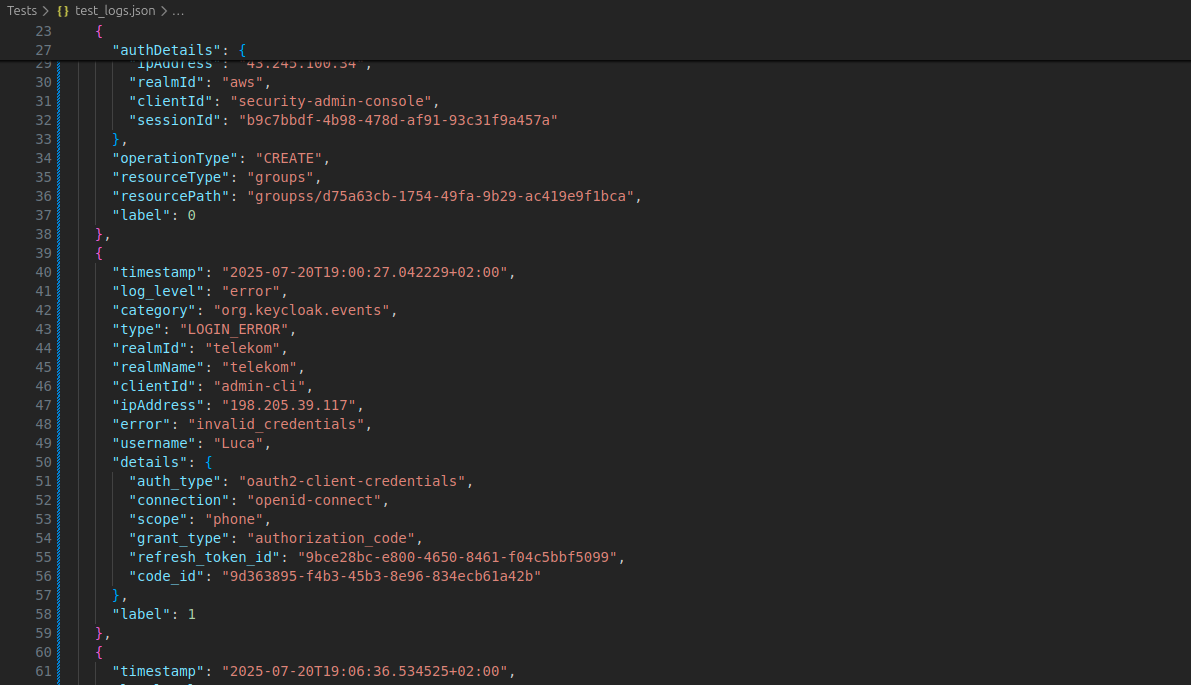
\includegraphics[width=1.0\linewidth]{Bilder/screenshot009}
		\caption{Ausschnitt der generierten Logs}
		\label{fig:screenshot009}
	\end{figure}
	Bei der Generierung der Log-Daten wurde auch berücksichtigt, dass neben eindeutig normalen und anomalen Sessions auch uneindeutige Sequenzen erzeugt werden, die als \textit{Noise} klassifiziert werden können. Solche Fälle treten in realen Systemen häufig auf – etwa wenn ein normaler Nutzer temporär priorisierte Rollen übernimmt oder häufig Passwörter ändert, ohne dass ein tatsächlicher Angriff vorliegt. Um eine zu starke Sensitivität der Modelle gegenüber solchen Mustern zu vermeiden, wird bewusst ein gewisser Anteil an Rauschen erzeugt.

	\subsection{Problematik dieser Lösung}
	Die Analyse basierte ausschließlich auf den wichtigsten, verfügbaren Log-Daten, die typische Systemaktivitäten und deren Merkmale widerspiegeln. Eine tiefere Untersuchung der internen Struktur und des vollständigen Aufbaus der Event-Typen in Keycloak war aufgrund fehlender umfassender Dokumentation und eingeschränktem Zugriff auf administrative Systemressourcen nicht möglich. Diese Einschränkungen begrenzen die Tiefe und Genauigkeit der Auswertung und können die Aussagekraft der Ergebnisse beeinflussen.
	\\[0.5em]
	Eine zentrale Herausforderung bestand in der realistischen Modellierung anomaler Sessions. Dabei musste unterschieden werden, ob eine Session normal, anormal oder als sogenannter \textit{Noise} einzustufen ist — also als legitimes, aber ungewöhnliches Verhalten, das fälschlich als Anomalie interpretiert werden könnte. Da echte Anomalien in der Realität selten auftreten, wurde bei der Datengenerierung heuristisch eine Auftrittswahrscheinlichkeit von 2,\,\% für anomale Sessions angenommen. Dadurch ist nicht gewährleistet, dass die erzeugten Daten eine realistischere Verteilung widerspiegeln.
	\\[0.5em]
	Ein weiterer Nachteil der synthetischen Generierung liegt darin, dass zufällig zusammengesetzte Ereignismuster entstehen können, die keinem realistischen Angriff entsprechen. Um dem entgegenzuwirken, wurde eine Logik implementiert, die grundlegende Systemregeln von Keycloak berücksichtigt: So darf ein Benutzer mit eindeutiger ID nur in einem Realm existieren, es gibt jeweils nur einen Administrator mit explizit definierten Rollen und höherer Priorität, und normale Benutzer können keine Operationen ausführen, die mit dem Attribut \textit{operationType} (CRUD-Operationen) verbunden sind — diese bleiben ausschließlich Administratoren vorbehalten. Zudem wird sichergestellt, dass jeder Benutzer genau einer Session und einem Realm zugeordnet ist, sofern es sich nicht explizit um einen Angreifer handelt.
	\\[0.5em]
	Aufgrund dieser Einschränkungen sowie der im späteren Verlauf beobachteten Resultate wurde der vorgestellte Ansatz zwar modellartig getestet, letztlich jedoch verworfen.
	
	\section{Möglichkeit 2: Datenbeschaffung als Alternative}
	Da die Generierung von Log-Daten mit hohem Aufwand verbunden ist, wurde stattdessen ein sinnvollerer Ansatz gewählt: die Beschaffung realer Keycloak-Daten (also direkt aus Keycloak selbst erzeugt). Aus datenschutzrechtlichen Gründen werden hierbei keine Daten aus Unternehmen verwendet. Stattdessen wurde die Idee verfolgt, eine lokale Keycloak-Instanz aufzusetzen und darauf basierend eigene Log-Daten zu generieren. Da auch dieser Weg zeitintensiv ist, wurde zusätzlich erwogen, mittels sogenannter \gls{selenium}-Tests sowohl Angriffsszenarien als auch gewöhnliche Keycloak-Daten zu simulieren. Als Grundlage zur Definition normaler Keycloak-Logs dient dabei eine Orientierung an firmeninternen Log-Daten.
	
	\subsection{Anbindung der Keycloak-API}
	Um Zugriff auf die Keycloak-Logs zu erhalten, ist es erforderlich, eine eigene Keycloak-Instanz zu installieren und sich mit Administratorrechten anzumelden. 
	\\[0.5em]
	Der Zugriff auf die Event-Logs erfolgt über die Keycloak-API, welche insbesondere bei der verwendeten Quarkus-Distribution eingesetzt wird. Standardmäßig benötigt man hierfür entsprechende Administrator-Rollen, um sensible Informationen wie Benutzer-Event-Logs und Administrator-Event-Logs abrufen zu können. Zunächst müssen die korrekten Authentifizierungsdaten vorliegen, um die erforderlichen Zugriffsrechte zu erhalten.
	\\[0.5em]
	Für die Authentifizierung wurde der sogenannte \textit{Client Credentials} Grant-Typ gewählt. Dabei erfolgt die Anmeldung über einen registrierten Client, wobei neben dem Client-Secret weitere Zugangsdaten übermittelt werden.

	\begin{figure}[H]
		\centering
		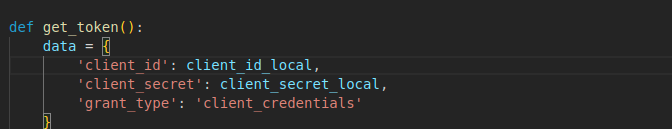
\includegraphics[width=0.9\linewidth]{Bilder/screenshot010}
		\caption{Daten, die an den Keycloak-Server gesendet werden müssen}
		\label{fig:screenshot010}
	\end{figure}
	Durch diesen Vorgang wird ein Zugriffstoken generiert, welches für den Abruf der Event-Logs benötigt wird. Das Token enthält Informationen zu den Zugriffsrechten des jeweiligen Administrators. So müssen beispielsweise die Rechte zum Verwalten von Benutzern enthalten sein, damit diese auch im Token ausgewiesen werden. Anschließend wird mit diesem Token eine weitere Anfrage an die API gestellt, um die Event-Logs abzurufen. Die erhaltenen Daten werden in einer separaten JSON-Datei gespeichert.
	\\[0.5em]
	Weitere Details zur Keycloak-API sind in der offiziellen Dokumentation zu finden \footnote{Keycloak Documentation, „REST API Reference“, \url{https://www.keycloak.org/docs-api/latest/rest-api/index.html}, letzter Zugriff: 30. Juli 2025.}.


	\subsection{Selenium-Tests zur Erzeugung der Logs}
	Selenium ist ein Framework zur automatisierten Ausführung von Webbrowser-Aktionen und als Python-Paket verfügbar. Es ermöglicht, Interaktionen mit der Benutzeroberfläche realitätsnah zu simulieren, sodass der Eindruck entsteht, ein Mensch bediene den Browser. Die wesentlichen Komponenten sind:
	
	\begin{itemize}
		\item \textbf{Selenium WebDriver}: Steuert den Browser programmgesteuert und stellt das zentrale Element der Tests dar.
		\item \textbf{Selenium Grid}: Ermöglicht die parallele Ausführung von Tests auf verschiedenen Maschinen und Browsern.
		\item \textbf{Selenium IDE}: Ein Recording-Tool im Browser, das jedoch für produktive oder komplexe Tests nicht empfohlen wird.
	\end{itemize}
	Für die Erstellung der Logs wird ausschließlich der WebDriver verwendet, der automatisch den Chrome-Browser startet. Die Wahl fiel auf Selenium, da es sich unkompliziert mit Keycloak verbinden lässt und sich gut für automatisierte Tests auf dieser Plattform eignet. Die Einrichtung gestaltet sich einfach: Es wird der zu verwendende Browser („Driver“) definiert und die Tests werden auf dem Port ausgeführt, auf dem die lokale Keycloak-Instanz erreichbar ist.
	\\[0.5em]
	Ein Nachteil dieser Methode liegt in der konstanten IP-Adresse, da alle Anfragen vom selben Host ausgehen. Dies kann dazu führen, dass das Modell lernt, mehrere Benutzer mit einer gemeinsamen IP-Adresse zu assoziieren, was in realen Szenarien als Anomalie interpretiert werden könnte. Daher wird die IP-Adresse vor der Weiterverarbeitung aus den Events entfernt. Diese Maßnahme reduziert zwar eine potenzielle Störquelle, verringert jedoch auch die Datenvielfalt für das Modell-besonders deshalb, weil die IP-Adresse als Feature gilt, welche mit Anomalien assoziiert sein kann.
	\\[0.5em]
	Außerdem erfolgt die Log-Erzeugung in kurzen zeitlichen Abständen, wodurch die zeitliche Streuung reduziert wird. Da das verwendete LSTM-Autoencoder-Modell zeitbasierte Muster analysiert, kann dies die Fähigkeit zur Anomalieerkennung einschränken. Zwar werden auch Tests zu ungewöhnlichen Uhrzeiten durchgeführt (z. B. abends), diese erzeugen jedoch nur wenige auffällige Logs.
	\\[0.5em]
	Trotz dieser Einschränkungen überwiegt der Vorteil, dass die erzeugten Logs den realen Keycloak-Logs sehr nahekommen – ein zentraler Aspekt, insbesondere wenn wirtschaftlich verwertbare Erkenntnisse aus dieser Arbeit gewonnen werden sollen. Die Testumgebung ermöglicht jedoch die Generierung geringerer Datenmengen (z. B. über 10.000 Events), was jedoch für das LSTM-Autoencoder-Modell ausreichend ist für das Training. Da die Logs direkt durch die definierten Tests erzeugt und gespeichert werden, entfällt die Notwendigkeit einer separaten manuellen Log-Generierung.
	
	\begin{figure}[H]
		\centering
		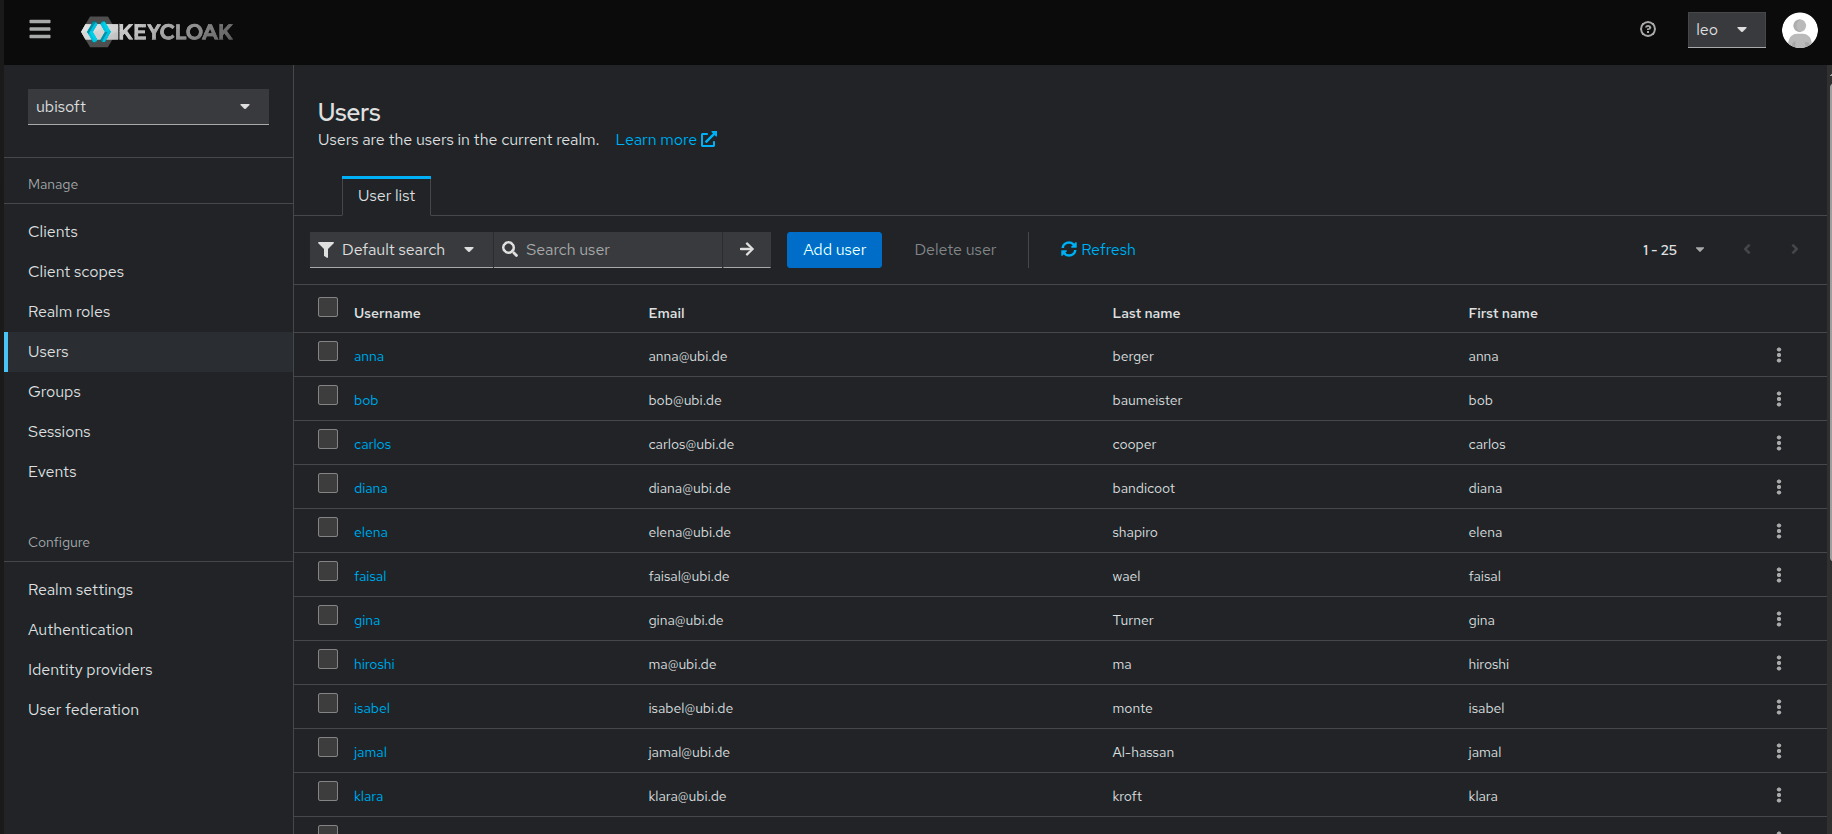
\includegraphics[scale=1.5, width=\linewidth]{Bilder/screenshot011}
		\caption{Beispielhafte Darstellung der generierten Benutzer für den Testfall}
		\label{fig:screenshot011}
	\end{figure}
	Zur Generierung der normalen Trainingsdaten wurden zuvor vier Realms erstellt:
	
	\begin{itemize}
		\item ubisoft
		\item Nintendo
		\item Sega
		\item aws
	\end{itemize}
	Pro Realm erfolgt die Benutzeranmeldung über einen jeweils definierten Client.
	\\[0.5em]
	Im Realm \textit{ubisoft} wurden 25 synthetische Benutzer erstellt, deren Namen alphabetisch generiert wurden (jeder Buchstabe des Alphabets außer „X“ ist vertreten). Für diesen Realm wurde der Client \textit{ps3} angelegt. Dieser ist erforderlich, damit sowohl Administratoren Zugriff auf die User-Events erhalten als auch Benutzer sich über diesen Client authentifizieren können. Um sicherzustellen, dass während der Selenium-Tests nicht auf den Master-Realm zugegriffen wird, muss für den Client eine passende \gls{redirecturl} definiert werden.
	\\[0.5em]
	In den weiteren Realms – \textit{Sega}, \textit{Nintendo} und \textit{aws} – wurden jeweils zehn Benutzer angelegt. Die zugehörigen Clients lauten: \textit{megadrive} (Sega), \textit{wii} (Nintendo) und \textit{aws-console} (aws).
	\\[0.5em]
	Jeder Realm verfügt über mindestens einen Administrator mit der Rolle \textit{realm-admin}. Ein Administrator, der für einen bestimmten Client Benutzer anlegen oder verwalten möchte, benötigt darüber hinaus die Rollen \textit{manage-users} und \textit{\gls{viewevents}}. Wichtig ist hierbei, dass diese Rollen nicht direkt den Benutzern, sondern den jeweiligen Clients zugewiesen werden. Dies liegt in der Architektur von Keycloak begründet: Clients besitzen eigene Zugriffsrechte, die ihnen bestimmte Operationen ermöglichen. So erlaubt die Rolle \textit{manage-users} dem Client, Benutzer im Realm programmatisch zu verwalten, während \textit{view-events} erforderlich ist, um Zugriff auf die Ereignisprotokolle zu erhalten – essenziell für Logging und Fehlersuche.
	\\[0.5em]
	Im Rahmen dieser Arbeit erzeugt ein Selenium-Test automatisch neue Benutzerkonten in Keycloak und weist ihnen jeweils ein Passwort zu. Diese Daten werden pro Realm einmalig in einer JSONL-Datei gespeichert, wobei Benutzername und Passwort als Schlüssel-Wert-Paar abgelegt werden.
	\\[0.5em]
	Damit sich die erzeugten Benutzer über die automatisierten Tests in Keycloak anmelden können, muss in der Konfiguration festgelegt werden, dass ein vollständiges Profil (Vorname, Nachname, E-Mail) erforderlich ist und vorhanden ist– andernfalls würde die Authentifizierung fehlschlagen.
	\\[0.5em]
	Darüber hinaus verfügen Clients dann über Service Accounts. Die Service-Account-Rollen bestimmen dabei die verfügbaren Rechte. Ohne diese Rollen könnte der Client zwar eine Verbindung herstellen, hätte jedoch keinen Zugriff auf Benutzerverwaltung oder Logdaten. Die korrekte Konfiguration der Service-Account-Rollen ist daher zwingend notwendig, um automatisierte Vorgänge im Hintergrund zu ermöglichen.
	
	\begin{figure}[H]
		\centering
		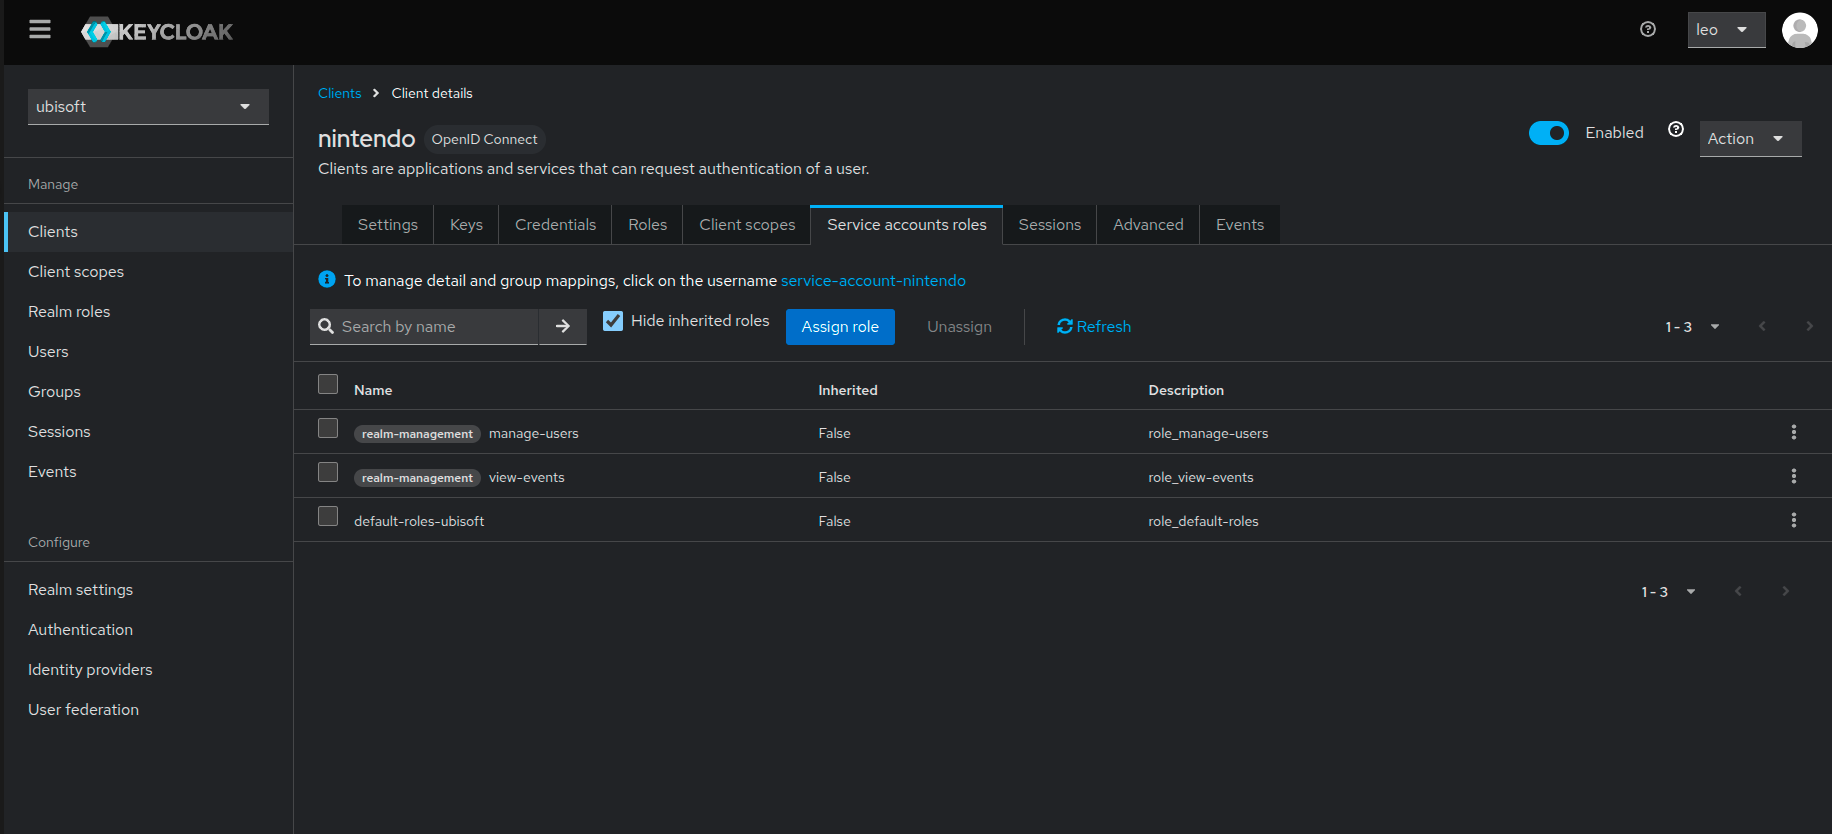
\includegraphics[width=0.9\linewidth]{Bilder/screenshot012}
		\caption{Benötigte Rollen für den Client Nintendo}
		\label{fig:screenshot012}
	\end{figure}
	Ab einer bestimmten Menge an Trainingsdaten werden die generierten Benutzer im Rahmen des Selenium-Tests dazu gebracht, sich regulär anzumelden. Die dabei entstehenden sogenannten „gewöhnlichen“ Logs umfassen unter anderem Anmeldevorgänge und basieren auf realen firmeninternen Protokollen. Diese bestehen typischerweise aus den Event-Typen LOGIN, CLIENT\_LOGIN und CODE\_TO\_TOKEN.
	\\[0.5em]
	Folgende Aktivitäten gelten laut interner Log-Analyse als „typisch“ nach dem Vergleich mit den firmeninternen Keycloak-Logs:
	
	\begin{itemize}
		\item Anmeldung über Keycloak direkt
		\item Anmeldung über einen Client
		\item Token-Aktualisierung (Refresh Token)
		\item Abmeldung (Logout), auch nach Ablauf einer Session
		\item Fehlgeschlagene Login-Versuche (kommen häufiger vor)
	\end{itemize}
	Weitere Aktionen – wie das Anpassen des Benutzerprofils (z. B. E-Mail-Änderung, Passwort-Zurücksetzung), das Löschen eines Clients oder das Zuweisen von Rollen an andere Benutzer beziehungsweise Clients – wurden in der Log-Generierung bewusst nicht automatisiert. Der Grund hierfür liegt in der vergleichsweise hohen Komplexität und der geringen Häufigkeit dieser Vorgänge. Da Keycloak primär als SSO-Dienst genutzt wird, wäre eine regelmäßige Durchführung solcher Aktionen im automatisierten Testkontext unrealistisch und würde die Aussagekraft der „normalen“ Logs verzerren.
	\\[0.5em]
	Stattdessen werden solche seltenen Aktionen manuell während des Testbetriebs von einzelnen Benutzern durchgeführt. Um dabei in die „Rolle“ eines anderen Benutzers zu schlüpfen, wird der Event-Typ \gls{impersonate} verwendet. Die Verwendung von Impersonation während der automatisierten Testausführung wird vermieden, da sie eine potenzielle Anomalie darstellt. Ziel ist es, lediglich gelegentlich und gezielt ungewöhnliche Aktionen zu erzeugen – etwa eine Passwort- oder E-Mail-Änderung, das Anlegen oder Löschen eines Benutzers oder das Zuweisen von Rollen. Dies reduziert den manuellen Aufwand bei der Erzeugung seltener Ereignisse, ohne die Gesamtdatenbasis zu verzerren.
	\\[0.5em]
	Pro Durchlauf werden insgesamt 30 Sessions (Bei den ersten 10000 Loggs waren es noch 15, wurde aber erhöht, um schneller Logs zu erzeugen) durchgeführt, wobei jede Session durch den häufigen Einsatz von Refresh Tokens mindestens zehn Einträge im Log erzeugt. Die Sitzungsdauer wird dabei durch die Konfiguration des jeweiligen Realms bestimmt. Aus praktischer Erfahrung ergibt sich eine durchschnittliche Dauer von etwa 35 Minuten pro Session – realistisch im Rahmen von 10 Minuten bis zu einer Stunde. So können am Tag zwischen 2.500 und 5.000 Log-Einträge erzeugt werden.
	\\[0.5em]
	Ereignisse, die typischerweise erst nach längerer Zeit auftreten, fehlen somit in der Testbasis. Eine spätere Erweiterung ist möglich, jedoch wurde aufgrund der Bearbeitungsfrist beschlossen, die Generierung auf 10 aufeinanderfolgende Tage zu konzentrieren, ausgeschlossen ist dabei das Wochenende. Die Sessions werden dabei nacheinander mit variablen Abstand ausgeführt.
	\\[0.5em]
	Nichtsdestotrotz stellt dieses Verfahren eine vorteilhafte Methode zur Log-Generierung dar, da die erzeugten Ereignisse die realen Keycloak-Logs darstellen.
	
		
	\subsection{Mögliche Angriffszenarien basierend auf \gls{cve} und \gls{cwe}}
	Common Vulnerabilities and Exposures (CVE) stellt eine umfassende Datenbank bekannter Sicherheitslücken dar, die in verschiedenen Softwaresystemen dokumentiert sind. Für Keycloak existieren ebenfalls zahlreiche veröffentlichte Schwachstellen\footnote{MITRE Corporation, „CVE Search Results for Keycloak“, \url{https://cve.mitre.org/cgi-bin/cvekey.cgi?keyword=keycloak}, letzter Zugriff: 30. Juli 2025.}
	\\[0.5em]
	CVE-Einträge liefern jedoch keine Lösungen, sondern dienen der transparenten und neutralen Information über Art, Ursache und potenzielle Auswirkungen der jeweiligen Sicherheitslücke. Jeder Eintrag erhält eine eindeutige Identifikationsnummer, eine Kurzbeschreibung sowie (sofern verfügbar) Angaben zur betroffenen Softwareversion. Die Pflege und Dokumentation erfolgt weltweit durch Organisationen, Forschungseinrichtungen sowie unabhängige Sicherheitsexperten.
	\\[0.5em]
	Im Gegensatz dazu beschreibt die Common Weakness Enumeration (CWE) systematisch bekannte Schwachstellenmuster (Weaknesses), die potenziell zu Sicherheitslücken führen können. Während CVEs konkrete, bereits gefundene oder ausgenutzte Schwachstellen auflisten, klassifiziert CWE abstrakte Fehlerklassen, wie beispielsweise „unzureichende Rechteprüfung“ oder „unsichere Tokenverarbeitung“. Beide Kataloge sind essentiell für die systematische Entwicklung und Interpretation von Sicherheitstests.
	\\[0.5em]
	Obwohl viele der bekannten Probleme bereits behoben wurden, zeigen sich Schwachstellen in Keycloak zunehmend wiederkehrend und entwickeln sich mit der Zeit weiter.
	\\[0.5em]
	Im Rahmen dieser Arbeit wurden mittels Selenium gezielt sicherheitsrelevante Angriffszenarien nach CVE und CWE und anderen Quellen (die schon im vorherigen Kapiteln bzgl. des ersten Entwurfes der Angriffsszenarien beschrieben wurden), gegen Keycloak simuliert und getestet. Es wird dabei folgendes Angriffsszenario umgesetzt: 
	\\[0.5em]
	\textbf{CVE-2024-3656 - \gls{privilegeescalation} in Keycloak}
	Bei CVE-2024-3656 \footnote{https://www.cve.news/cve-2024-3656/} handelt es sich um eine Sicherheitslücke in Keycloaks Admin REST API, bei der unzureichende Berechtigungsprüfungen es einem Nutzer mit niedrigen Rechten ermöglichen, administrative Endpunkte aufzurufen. Dadurch können sensible Daten wie Benutzerlisten eingesehen und administrative Aktionen durchgeführt werden, ohne dass entsprechende Rechte vorliegen. Die Ursache liegt in fehlerhaften oder fehlenden Zugriffskontrollen auf kritischen API-Endpunkten. Die Schwachstelle wurde in neueren Keycloak-Versionen behoben, darunter auch die Version 26.1.0, welche in dieser Arbeit verwendet wird. Andere Angriffsfälle konnten nicht umgesetzt werden, da manche Features die dafür verlangt werden in aktuellen oder früheren Versionen nicht mehr erhältlich sind. Auch wenn dieser Angriff fehlschlägt- sorgt er dafür, dass viele Logs mit anomalen Charakter generiert werden.
	\\[0.5em]
	Da CVE-Datenbanken keine vollständigen Exploitbeschreibungen liefern, wurde im Rahmen der Simulation eine technische Interpretation der Schwachstellen vorgenommen. Zudem wurden noch weitere Angriffe ausgeführt,welche Typisch sind für einen Angriff und auch schon in den bekannten Insiderangriffsfällen genannt wurde:
	\begin{itemize}
		\item \textbf{\gls{accountsabotage}-Test: }  
		Löschen oder Verändern wichtiger Benutzerinformationen.
		\item \textbf{Brute Force Angriff}
	\end{itemize}

	\subsection{Angriffsszenarien}                         
	Die im vorherigen Abschnitt beschriebenen Angriffsszenarien wurden im Rahmen dieser Arbeit mithilfe von Selenium-Tests implementiert und in den generierten Logs dokumentiert. Für jedes Szenario wurde ein konkreter Ablauf definiert, um die jeweilige Sicherheitslücke zu simulieren.
	\\[0.5em]
	Hier werden die Angriffsfälle aufgelistet welche direkt in der Keycloak-Konsole ausgeführt wurden, also nicht als Selenium-Test- außer das erste Szenario des Testfalls \textit{Privilege Escalation}, dieses wird auch als Selenium-Test ausgeführt.
	
	\subsubsection{Angriffsszenario: Versuch einer Privilege Escalation über die Admin REST API}
	
	In diesem Szenario wird untersucht, ob ein technisch privilegierter, aber nicht vollständig administrativer Benutzer in Keycloak durch gezielte API-Aufrufe seine eigenen Berechtigungen ausweiten kann. Ziel ist es, das Verhalten von Keycloak bei einer möglichen Rechteausweitung über die REST-Schnittstelle zu evaluieren.
	
	\begin{description}
		\item[Ziel:] Unautorisierte Erweiterung der Benutzerrechte durch Ausnutzung der REST API
		\item[Betroffener Realm:] \texttt{Ubisoft}
		\item[Angreiferrolle:] Benutzer mit der Rolle \texttt{manage-users}
		\item[Betroffener Benutzer:] \texttt{bob} (versucht sich selbst administrative Rechte zu geben)
	\end{description}
	
	\paragraph{Ablauf:}
	\begin{enumerate}
		\item Der Benutzer \texttt{bob} meldet sich regulär im System an und verfügt über ein gültiges Access Token.
		\item Mit diesem Token führt er einen \texttt{GET}-Request auf \texttt{/admin/realms/ubisoft/users} aus, um die Benutzerliste des Realms zu erhalten.
		\item Die Abfrage ist erfolgreich – bob erhält Zugriff auf die vollständige Liste und identifiziert seine eigene Benutzer-ID.
		\item Anschließend versucht er über einen \texttt{POST}-Request an \texttt{/admin/realms/ubisoft/users/\{id\}/role-mappings/realm}, sich selbst die Rolle \texttt{realm-admin} zuzuweisen.
		\item Der Request schlägt fehl – die Serverantwort ist \texttt{HTTP 401 Unauthorized}.
	\end{enumerate}
	
	\paragraph{Technische Umsetzung:}
	Die Requests wurden mithilfe von \texttt{curl} direkt an die REST API gesendet. Dabei wurde ein korrekt signiertes Access Token verwendet, das bob durch einen Login mit seiner \texttt{manage-users}-Rolle erhalten hatte.
	
	\paragraph{Erwartetes Verhalten:}
	\begin{itemize}
		\item Die Benutzerliste kann durch Rollen wie \texttt{manage-users} teilweise eingesehen werden, was ein potenzielles Datenschutzrisiko darstellt.
		\item Die unautorisierte Zuweisung privilegierter Rollen wird vom Server korrekt abgelehnt.
		\item Der Zugriff auf administrative Rollen über die REST API ist in Keycloak Version 26.1 restriktiver als in früheren Versionen, was diese Art von Privilege Escalation wirksam verhindert.
	\end{itemize}
	
	\paragraph{Sicherheitsrelevanz:}
	Das Szenario zeigt, dass selbst privilegierte Benutzer mit erweiterten Rechten (z.\,B. \texttt{manage-users}) keine vollständigen administrativen Aufgaben übernehmen können. Dennoch bleibt der Zugriff auf sensible Informationen wie Benutzerlisten ein Risiko. Frühere Keycloak-Versionen waren anfällig für ähnliche Angriffe (z.\,B. \texttt{CVE-2024-3656}). Seit Version 26.1 wurden entsprechende Sicherheitsmechanismen gestärkt, um Missbrauch über die REST API zu verhindern.
	
	\subsubsection{Angriffsszenario: Account-Sabotage durch privilegierten Benutzer}
	In diesem Szenario wird untersucht, inwieweit ein privilegierter Benutzer (z.\,B. ein Administrator) absichtlich oder versehentlich Schaden an Benutzerkonten anrichten kann. Ziel ist es, das Verhalten von Keycloak bei kritischen administrativen Operationen zu beobachten und zu analysieren, welche Aktionen protokolliert werden.
	
	\begin{description}
		\item[Ziel:] Simulierte Account-Sabotage durch einen legitimen Admin im Realm
		\item[Betroffener Realm:] \texttt{Sega}
		\item[Angreiferrolle:] Benutzer mit Administratorrechten (z.\,B. \texttt{realm-admin} oder \texttt{manage-users})
		\item[Betroffene Benutzer:] \texttt{Admin in Sega} (Profiländerung) sowie drei zufällige Benutzer (Löschung)
	\end{description}
	
	\paragraph{Ablauf:}
	\begin{enumerate}
		\item Ein Angreifer kennt die Credentials des Admins im Realm \texttt{Sega} und ist bereits mit dessen Credentials eingeloggt.
		\item Der Angreifer ändert das Passwort des Admins in Sega.
		\item Anschließend löscht der Admin drei beliebige Benutzerkonten im selben Realm.
		\item Der falsche Admin meldet sich ab.
	\end{enumerate}
	
	\paragraph{Technische Umsetzung:}
	Die Ausführung erfolgt entweder manuell über die Keycloak Admin Console oder automatisiert mit Hilfe von \texttt{Selenium}.
	
	\paragraph{Erwartetes Verhalten:}
	\begin{itemize}
		\item Die Profiländerungen und das Zurücksetzen des Passworts sollten als \texttt{UPDATE\_PASSWORD} im \textbf{User-Event-Log} erscheinen.
		\item Die Löschung der Benutzerkonten wird im \textbf{Admin-Event-Log} als \texttt{DELETE} Operation registriert.
		\item Alle Aktionen sind über den Zeitstempel, Benutzer und IP-Adresse nachvollziehbar.
		\item \textit{LOGOUT} wird ebenfalls in den Logs angezeigt
	\end{itemize}
	
	\paragraph{Sicherheitsrelevanz:}
	Dieses Szenario demonstriert, wie gefährlich ein missbrauchter Admin-Zugang sein kann. In realen Umgebungen sollten Änderungen durch Admins auditiert und mit mehrstufigen Genehmigungsmechanismen oder Alerting-Systemen abgesichert sein.

	\subsubsection{Angriffsszenario: Brute-Force-Angriff über die Web-Oberfläche}
	In diesem Szenario wird ein klassischer Brute-Force-Angriff simuliert, bei dem ein Benutzername fest vorgegeben ist und systematisch unterschiedliche Passwörter ausprobiert werden. Ziel ist es zu prüfen, ob ein erfolgreiches Login durch mehrfaches Raten von Passwörtern möglich ist und ob Keycloak entsprechende Fehlversuche protokolliert.
	
	\begin{description}
		\item[Ziel:] Test der Account-Sicherheit gegenüber einfachen Brute-Force-Angriffen über das Login-Formular
		\item[Betroffener Benutzer:] \texttt{admin}
		\item[Realm:] Dynamisch gewählt (aus mehreren Realms auswählbar)
		\item[Passwortliste:] Eine Liste gängiger schwacher Passwörter (z.\,B. \texttt{admin123}, \texttt{123456}, \texttt{password}, \texttt{qwerty}, \texttt{welcome}, etc.)
	\end{description}
	
	\paragraph{Ablauf:}
	\begin{enumerate}
		\item Es wird eine Verbindung zur Keycloak-Login-Seite des jeweiligen Realms hergestellt.
		\item Der Benutzername wird in das Formular eingetragen (\texttt{admin}).
		\item Es wird nacheinander jedes Passwort aus der vorgegebenen Liste eingegeben und die Login-Schaltfläche betätigt.
		\item Das Skript prüft, ob eine Fehlermeldung erscheint oder ob der Login erfolgreich war.
		\item Bei Erfolg wird der Versuch gestoppt.
	\end{enumerate}
	
	\paragraph{Technische Umsetzung:}
	Die Automatisierung erfolgt mittels \texttt{Selenium WebDriver} in Kombination mit einer Python-Testfunktion. Die Login-Seite wird jeweils mit einem neuen Passwort geladen und automatisiert ausgefüllt.
	
	\paragraph{Erwartetes Verhalten:}
	\begin{itemize}
		\item Keycloak sollte nach mehreren Fehlversuchen Gegenmaßnahmen ergreifen (z.\,B. Account-Sperrung, Rate Limiting).
		\item Im Event-Log sollten die fehlgeschlagenen Login-Versuche als \texttt{LOGIN\_ERROR} mit dem jeweiligen Benutzer verzeichnet sein.
	\end{itemize}
	Brute Force und Privilege Escalation sind Angriffe, die fehlschlagen. Nur Account Sabotage ist erfolgreich. Dies ligt an der Umsetzung (Brute Force durch Selenium-Tests) und daran, dass der erwähnte CVE Fall für neuere Keycloak Versionen nicht mehr funktioniert durch neue Sicherheitsfunktionen- dennoch stellen sie erkennbare, anomale Logs dar.
	
	\paragraph{Sicherheitsrelevanz:}
	Ein solcher Angriff simuliert reale Angriffsvektoren durch Bots oder Skripte. Das Vorhandensein und die Konfiguration von Mechanismen wie \textit{Brute Force Detection}, Lockout Policies oder IP-Rate-Limits sind für die Sicherheit von zentraler Bedeutung.

	\section{Durchführung des Trainings}
	Die Logs werden separat je nach Training, Test und Validierung in Dateien gepackt und dann zu Beginn ausgelesen. Zuerst werden diese Daten vorverarbeitet. Die Features werden danach automatisch in numerische, kategorische oder nicht definierte Daten eingeteilt. Die eingeteilten und bereinigten Daten werden danach wieder zusammengefügt. Alle drei Dateien, also Evaluierungs-, Test- und Trainingsdateien werden dabei einzeln bereinigt und zusammengefügt. Darauf hin werden alle Daten mit der standardisiert und skaliert. Da der LSTM-AE nur mit sequentiellen Daten arbeiten kann, wurden diese Dateien in Sequenzen aufgeteilt.
	\\[0.5em]
	Über einen Zeitraum von 12 Tagen (2.5 Wochen, nur Werktage) wurden ausschließlich „normale“ Logs generiert. An den darauffolgenden Tagen fanden gezielte Angriffsszenarien statt. Mithilfe eines Skripts wurden anschließend sämtliche Event-Logs aus allen Realms zusammengeführt.
	\\[0.5em]
	Die kombinierten Logs wurden zunächst im Verhältnis 70\,\% zu Trainingsdaten und jeweils 15\,\% zu Test- und Validierungsdaten aufgeteilt. Die Anomalien wurden zufällig auf die Test- und Validierungsdaten verteilt, dabei jedoch in zeitlich korrekter Reihenfolge einsortiert. Da die Anomalien erst nachträglich erzeugt wurden, mussten die Timestamps entsprechend angepasst werden.
	\\[0.5em]
	Eine rein zufällige Vergabe der Timestamps war dabei nicht möglich, da bestimmte Angriffsszenarien einen klaren zeitlichen Ablauf erfordern. Die Timestamps wurden daher gezielt so angepasst, dass sie diesen inhaltlichen Zusammenhang korrekt abbilden, ohne am Ende des Datensatzes zu kumulieren. Aufgrund der überschaubaren Anzahl an Anomalien (ca. 50–70 Einträge) konnte dieser Schritt manuell umgesetzt werden.
	\\[0.5em]
	Bevor die anomalen Logs mit den normalen vermischt wurden, fügte das Skript Labelinformationen hinzu: In der Datei attacks\_logs.py wurden die anomalen Ereignisse aus Keycloak extrahiert und mit dem Label "1" versehen, während in der Datei normal\_test\_logs.py die regulären Log-Einträge mit dem Label "0" markiert wurden.
	\\[0.5em]
	Abschließend wurde die finale Datei in zwei Hälften aufgeteilt; in eine Validierung- und einer Testdatei.
	\\[0.5em]
	Das LSTM-AE wird dabei nur mit normalen Daten trainiert. Wie viele Trainingsdaten an sich auch nötig sind, ist ein weitgehend offenes Problem. Es gibt nur wenige Studien, die sich systematisch mit der Frage beschäftigt haben, welche Datenmenge „angemessen“ ist, um ein neuronales Netzwerk zuverlässig zu trainieren.
	\\[0.5em]
	Nach der Studie von Golestaneh et al. \cite{Golestaneh2021} wurde eine theoretische Fehlerabschätzung für bestimmte Netzwerke abgeleitet. Demnach skaliert der Fehler $\varepsilon$ eines solchen Netzwerks nicht mit der klassischen „parametrischen“ Rate von $\varepsilon \sim 1/n$, sondern mit einer langsameren, linearen Rate:
	
	\[
	\varepsilon(n) \sim \frac{1}{\sqrt{n}}
	\]
	Dabei ist \(n\) die Anzahl der Trainingsbeispiele. Diese Formel bedeutet, dass eine Verdopplung der Datenmenge den Fehler nicht halbiert, sondern nur um den Faktor \(1/\sqrt{2}\) verringert. Dennoch erlaubt diese Abschätzung eine grobe Einschätzung der notwendigen Datenmenge.
	\\[0.5em]
	Wendet man diese Formel auf eine Trainingsmenge von $n = 10.000$ Log-Zeilen an, ergibt sich ein theoretischer Fehler von etwa
	
	\[
	\varepsilon(10.000) \approx \frac{1}{\sqrt{10.000}} = 0{,}01
	\]
	Dieser Wert gilt zwar nicht als absolute Fehlermarke (da der tatsächliche Fehler von Modellarchitektur, Datenqualität und Regularisierung abhängt), er ist jedoch in vielen praktischen Fällen bereits hinreichend gering, um eine sinnvolle Modellierung zu ermöglichen. Somit kann ein LSTM-Autoencoder bei geeigneter Modellwahl und sauberem Datenvorverarbeitung bereits mit etwa 10.000 normalisierten Log-Zeilen ein brauchbares Modell für Anomalieerkennung liefern.
	\\[0.5em]
	Auch eine weitere Studie von Götz et al. \cite{Goetz2023} beschäftigt sich mit der Relation zwischen der Komplexität eines neuronalen Netzwerks (gemessen an der Anzahl der trainierbaren Parameter \( N_p \)) und der Anzahl der notwendigen Trainingsbeispiele \( N_{tr} \). Dabei wurde gezeigt, dass kein starres Verhältnis wie \( N_{tr} \geq N_p \) erforderlich ist, um gute Ergebnisse zu erzielen. Stattdessen weisen die Autoren nach, dass auch mit deutlich weniger Trainingsbeispielen eine stabile Modellleistung möglich.
	\\[0.5em]
	In ihren Experimenten mit Convolutional Neural Networks (CNNs) konnten selbst bei einem Verhältnis \( N_{tr}/N_p < 1 \) noch vergleichbare Klassifikationsleistungen erzielt werden, solange die Reduktion der Netzwerkkomplexität kontrolliert erfolgt. Übertragen auf den vorliegenden Fall bedeutet dies: Bei einem moderat komplexen LSTM-Autoencoder mit z.\,B. einigen zehntausend Parametern können bereits $10.000$ Trainingsbeispiele (z.\,B. Log-Zeilen) ausreichen, um ein funktionierendes Modell zu erhalten – sofern geeignete Regularisierung und Modellarchitektur verwendet werden. 
	\\[0.5em]
	Die Studie stützt damit ebenfalls die Annahme, dass in vielen praktischen Szenarien bereits Datensätze im Bereich von 10.000 bis 50.000 Einträgen als ausreichend gelten können, um eine robuste Anomalieerkennung durchzuführen-wobei man natürlich beachten muss, dass in jeder Studie der Fokus auf einem anderen Netzwerk lag. Bspw. basiert Golestanehs Formel auf ReLU-basierte Netzwerke. Dennoch will man diese Studien als Hinweis dafür wahrnehemn, möglichst viele Daten zu generieren, auch wenn es im Rahmen dieser Arbeit die Anzahl der wahrscheinlich nur im fünf-stelligen Bereich liegen wird.
	\\[0.5em]
	Auf Grundlage dieser Erkenntnisse wird ein Testfall mit ca. 39000 Logs erstellt.
	\\[0.5em]
	Für den Testfall wurde mit 50 und 100 Epochen trainiert. Für den Test befinden sich in den Test - und Validierungsdaten befinden sich ca. 31 Log-Einträge, welche durch je eines der fünf Angriffsszenarien entsteht.

	\subsection{Änderung der Timestamps durch Unix Timestamp}
	Da die Timestamps manuell geändert werden müssen, muss gewährleistet sein, dass diese zufällig vom 22.07,ca. 14 Uhr bis zum 08.08, 17 Uhr erzeugt wurden- und demnach verändert werden. Es wurden folgende Zeitpunkte pro Angriffsszenario modelliert:
	\begin{itemize}
		\item \textit{Brute Force Angriff:} Umstellung auf den 06.08 um 13 Uhr Abends
		\item \textit{Privilege Escalation:} Umstellung auf den 07.08 um 16 Uhr
		\item \textit{Account Sabotage:} Umstellung auf den 08.08 um 11 Uhr Morgens
	\end{itemize}
	Diese Zeitpunkte werden auf der Webseite Unix Timestamp \footnote{https://www.unixtimestamp.com/} verändert.
	
	\begin{figure}[H]
		\centering
		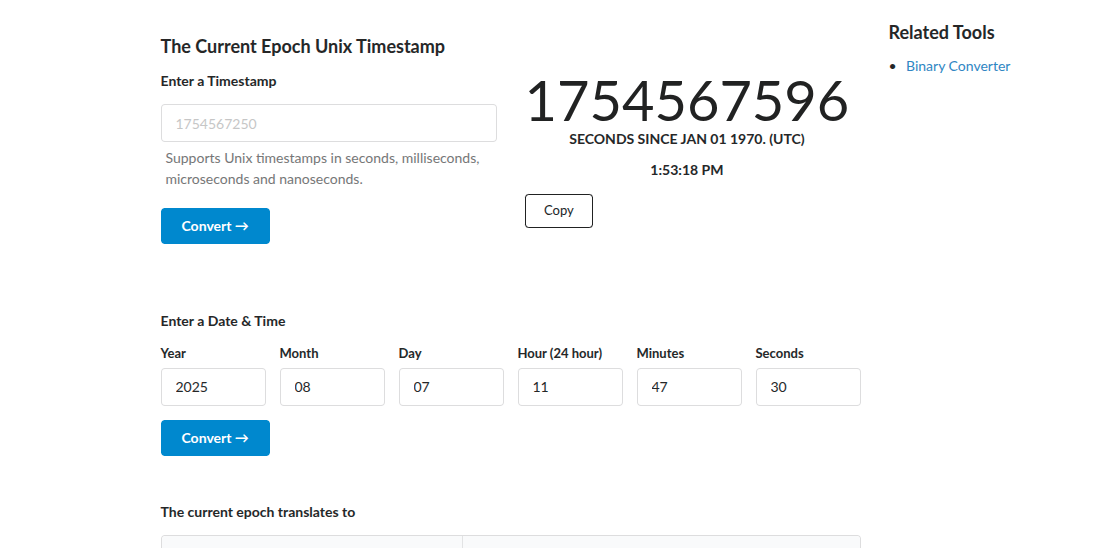
\includegraphics[width=0.9\linewidth]{Bilder/screenshot019}
		\caption{Aktuelle Uhrzeit nach dem Unix-System}
		\label{fig:screenshot019}
	\end{figure}
	Die erste Attacke dauert ca. 1-2 Minuten, die zweite ca. 5-10 Minuten und die letzte im ca. 20 Minuten. Dies Zeit wurde so bestimmt,dass sie sich für den jeweiligen Angriff eignen. Die Angriffe werden mit Absicht an Zeitpunkte durchgeführt, welche zwischen den normalen Logs mit Abstand sind, damit das LSTM-AE auch seinen Einsatz daran zeigen kann. Denn bei zu kurzen Sequenzen und auch plötzlichen, würde das LSTM-AE nur bei einer viel zu kurzen Sequenzlänge an Aussagekraft verlieren.
	
	\subsection{Testfälle}
	Aufgrund der ungleichmäßigen Verhältnis zwischen Anomalien und normalen Logs und der geringen Anzahl an Logs wurde beschlossen Testfälle mit unterschiedlichen Architekturen durchzugehen.
	Es werden folgende Sequenzlängen validiert:
	\begin{itemize}
		\item Sequenzlänge 10
		\item Sequenzlänge 25
		\item Sequenzlänge 50
	\end{itemize}
	Die Wahl der unterschiedlichen Sequenzlängen dient dazu, die Sensitivität des Modells auf verschiedene zeitliche Zusammenhänge zu testen. Kürzere Sequenzen erfassen lokale Muster, während längere Sequenzen komplexere zeitliche Abhängigkeiten abbilden können. Dadurch kann das Modell besser an die unterschiedlichen Charakteristika der Log-Daten angepasst werden.
	\\[0.5em]
	Die Labels kennzeichnet jeden Log-Eintrag als Anomalie (1) oder normal (0). Alle weiteren Log-Merkmale wie Eventtyp oder Zeitstempel werden als unabhängige Variablen in das Modell eingespeist.
	\\[0.5em]
	Die Architektur selbst beinhaltet schon Störfaktoren. Tiefe, Breite und auch die Batch-Size beeinflussen viel von dem, wie die Modelle insgesamt arbeiten.
	\\[0.5em]
	Zur Übersicht wurden Tabellen erstellt,welche das Verhältnis zu den abhängigen und unabhängigen Variablen zeigen soll:
	\\[0.5em]
	Variablen der Hybridmodelle:
	
	\begin{figure}
		\centering
		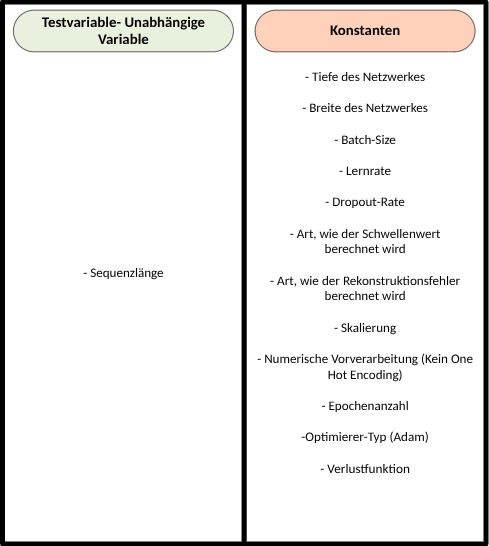
\includegraphics[width=1.1\linewidth]{Bilder/variablen-architektur}
		\caption{Überblick der Konstanten Werte und der unabhängigen Variable}
		\label{fig:variablen-architektur}
	\end{figure}

	Die Architektur des LSTM-Autoencoders wird bewusst minimal gehalten. Die Sequenzlänge wird auf 10 Log-Einträge gesetzt, um lokale zeitliche Muster effizient zu erfassen, ohne die Netzwerkkomplexität unnötig zu erhöhen. Die Batch-Size wird konstant auf 32 gehalten, da sie einen guten Kompromiss zwischen stabiler Gradientenberechnung und Trainingsgeschwindigkeit bietet und bei der Gesamtzahl von 39.000 Logeinträgen ausreichend robuste Updates ermöglicht.
	\\[0.5em]
	Die Encoder- und Decoder-Layer sind jeweils mit [128, 64] bzw. [64, 128] Neuronen konfiguriert, wodurch das Modell leichtgewichtig bleibt und Overfitting vermieden wird, während gleichzeitig die typischen Muster in den Log-Sequenzen zuverlässig erfasst werden können. Dropout wird deaktiviert, um die Reproduzierbarkeit der Ergebnisse zu gewährleisten, sodass jeder Trainingsdurchlauf unter identischen Bedingungen erfolgt. Die Lernrate wird auf 0,001 gesetzt, ein bewährter Startwert, der stabile Konvergenz in Kombination mit der gewählten Architektur und Batch-Size erlaubt.
	\\[0.5em]
	Weitere Faktoren wie die Berechnung des Rekonstruktionsfehlers, der Schwellenwert, die Skalierung (StandardScaler), die Anzahl der Trainings-Epochen (50), der Optimierer (Adam) und die Verlustfunktion (MSE) werden konstant gehalten, um einen fairen Vergleich der Modelle zu gewährleisten. Die gewählten Konstanten können zwar die erzielbaren Höchstwerte im Vergleich zu anderen Studien begrenzen, gewährleisten jedoch, dass die Analyse zuverlässig und nachvollziehbar bleibt.
	\\[0.5em]
	Kurz gesagt: Die abhängige Variable hier stellen die Metriken dar in den Logs dar, die unabhängige die Sequenzlänge.
	
	\section{Ergebnisse}
	\subsection{Ergebnisse mit der Sequenzlänge 10}
	\subsubsection{Testlauf 1}
	\begin{table}[H]
		\centering
		\begin{tabular}{lc}
			\hline
			Metrik & Wert \\
			\hline
			Best Threshold (F1) & 0.1861 \\
			Precision & 0.9519 \\
			Recall & 0.7734 \\
			F1 & 0.8534 \\
			ROC-AUC & 0.9630 \\
			AUC-PR & 0.7412 \\
			Matthews Correlation Coefficient (MCC) & 0.8553 \\
			Balanced Accuracy & 0.8863 \\
			\hline
		\end{tabular}
		\caption{Ergebnisse für IsolationForest}
	\end{table}
	
	% Tabelle für One-Class SVM
	\begin{table}[H]
		\centering
		\begin{tabular}{l c}
			\hline
			Metrik & Wert \\
			\hline
			Best Threshold (F1) & 4999.3471 \\
			Precision & 0.9364 \\
			Recall & 0.8047 \\
			F1 & 0.8655 \\
			ROC-AUC & 0.9109 \\
			AUC-PR & 0.7577 \\
			Matthews Correlation Coefficient (MCC) & 0.8654 \\
			Balanced Accuracy & 0.9017 \\
			\hline
		\end{tabular}
		\caption{Ergebnisse für One-Class SVM}
	\end{table}
	
	% Tabelle für DBSCAN
	\begin{table}[H]
		\centering
		\begin{tabular}{l c}
			\hline
			Metrik & Wert \\
			\hline
			Best Threshold (F1) & 2.0099 \\
			Precision & 1.0000 \\
			Recall & 0.1484 \\
			F1 & 0.2585 \\
			ROC-AUC & 0.5742 \\
			AUC-PR & 0.1670 \\
			Matthews Correlation Coefficient (MCC) & 0.3817 \\
			Balanced Accuracy & 0.5742 \\
			\hline
		\end{tabular}
		\caption{Ergebnisse für DBSCAN}
	\end{table}
	\subsubsection{Testlauf 2}
	
	\begin{table}[H]
		\centering
		\begin{tabular}{l c}
			\hline
			Metrik & Wert \\
			\hline
			Best Threshold (F1) & 0.1850 \\
			Precision & 0.9903 \\
			Recall & 0.7969 \\
			F1 & 0.8831 \\
			ROC-AUC & 0.9638 \\
			AUC-PR & 0.7936 \\
			Matthews Correlation Coefficient (MCC) & 0.8862 \\
			Balanced Accuracy & 0.8984 \\
			\hline
		\end{tabular}
		\caption{Ergebnisse für IsolationForest}
	\end{table}
	
	\begin{table}[H]
		\centering
		\begin{tabular}{l c}
			\hline
			Metrik & Wert \\
			\hline
			Best Threshold (F1) & 5444.4513 \\
			Precision & 0.9903 \\
			Recall & 0.7969 \\
			F1 & 0.8831 \\
			ROC-AUC & 0.9184 \\
			AUC-PR & 0.7936 \\
			Matthews Correlation Coefficient (MCC) & 0.8862 \\
			Balanced Accuracy & 0.8984 \\
			\hline
		\end{tabular}
		\caption{Ergebnisse für One-Class SVM}
	\end{table}
	
	\begin{table}[H]
		\centering
		\begin{tabular}{l c}
			\hline
			Metrik & Wert \\
			\hline
			Best Threshold (F1) & 2.0995 \\
			Precision & 1.0000 \\
			Recall & 0.1250 \\
			F1 & 0.2222 \\
			ROC-AUC & 0.5625 \\
			AUC-PR & 0.1441 \\
			Matthews Correlation Coefficient (MCC) & 0.3502 \\
			Balanced Accuracy & 0.5625 \\
			\hline
		\end{tabular}
		\caption{Ergebnisse für DBSCAN}
	\end{table}
	
	\subsubsection{Testlauf 3}
	
	\begin{table}[H]
		\centering
		\begin{tabular}{l c}
			\hline
			Metrik & Wert \\
			\hline
			Best Threshold (F1) & 0.1934 \\
			Precision & 0.9196 \\
			Recall & 0.8047 \\
			F1 & 0.8583 \\
			ROC-AUC & 0.9584 \\
			AUC-PR & 0.7443 \\
			Matthews Correlation Coefficient (MCC) & 0.8574 \\
			Balanced Accuracy & 0.9016 \\
			\hline
		\end{tabular}
		\caption{Ergebnisse für IsolationForest}
	\end{table}
	
	\begin{table}[H]
		\centering
		\begin{tabular}{l c}
			\hline
			Metrik & Wert \\
			\hline
			Best Threshold (F1) & 4082.3180 \\
			Precision & 0.9043 \\
			Recall & 0.8125 \\
			F1 & 0.8560 \\
			ROC-AUC & 0.9168 \\
			AUC-PR & 0.7389 \\
			Matthews Correlation Coefficient (MCC) & 0.8542 \\
			Balanced Accuracy & 0.9053 \\
			\hline
		\end{tabular}
		\caption{Ergebnisse für One-Class SVM}
	\end{table}
	
	\begin{table}[H]
		\centering
		\begin{tabular}{l c}
			\hline
			Metrik & Wert \\
			\hline
			Best Threshold (F1) & 2.0106 \\
			Precision & 1.0000 \\
			Recall & 0.2188 \\
			F1 & 0.3590 \\
			ROC-AUC & 0.6094 \\
			AUC-PR & 0.2358 \\
			Matthews Correlation Coefficient (MCC) & 0.4637 \\
			Balanced Accuracy & 0.6094 \\
			\hline
		\end{tabular}
		\caption{Ergebnisse für DBSCAN}
	\end{table}
	
		
	\subsubsection{Ergebnisse mit der Sequenzlänge 25}
	\subsubsection{Testdurchlauf 1}
	\begin{table}[H]
		\centering
		\begin{tabular}{l c}
			\hline
			Metrik & Wert \\
			\hline
			Best Threshold (F1) & 0.1764 \\
			Precision & 0.9290 \\
			Recall & 0.6305 \\
			F1 & 0.7512 \\
			ROC-AUC & 0.9408 \\
			AUC-PR & 0.6015 \\
			Matthews Correlation Coefficient (MCC) & 0.7574 \\
			Balanced Accuracy & 0.8142 \\
			\hline
		\end{tabular}
		\caption{Ergebnisse für IsolationForest, Sequenzlänge 25}
	\end{table}
	
	\begin{table}[H]
		\centering
		\begin{tabular}{l c}
			\hline
			Metrik & Wert \\
			\hline
			Best Threshold (F1) & 6275.1389 \\
			Precision & 0.9401 \\
			Recall & 0.6305 \\
			F1 & 0.7548 \\
			ROC-AUC & 0.8532 \\
			AUC-PR & 0.6085 \\
			Matthews Correlation Coefficient (MCC) & 0.7622 \\
			Balanced Accuracy & 0.8144 \\
			\hline
		\end{tabular}
		\caption{Ergebnisse für One-Class SVM, Sequenzlänge 25}
	\end{table}
	
	\begin{table}[H]
		\centering
		\begin{tabular}{l c}
			\hline
			Metrik & Wert \\
			\hline
			Best Threshold (F1) & 2.2846 \\
			Precision & 1.0000 \\
			Recall & 0.0442 \\
			F1 & 0.0846 \\
			ROC-AUC & 0.5221 \\
			AUC-PR & 0.0848 \\
			Matthews Correlation Coefficient (MCC) & 0.2059 \\
			Balanced Accuracy & 0.5221 \\
			\hline
		\end{tabular}
		\caption{Ergebnisse für DBSCAN, Sequenzlänge 25}
	\end{table}
	
	\subsubsection{Testlauf 2}
	
	\begin{table}[H]
		\centering
		\begin{tabular}{l c}
			\hline
			Metrik & Wert \\
			\hline
			Best Threshold (F1) & 0.1735 \\
			Precision & 0.9811 \\
			Recall & 0.6265 \\
			F1 & 0.7647 \\
			ROC-AUC & 0.9410 \\
			AUC-PR & 0.6306 \\
			Matthews Correlation Coefficient (MCC) & 0.7771 \\
			Balanced Accuracy & 0.8130 \\
			\hline
		\end{tabular}
		\caption{Ergebnisse für IsolationForest, Sequenzlänge 25}
	\end{table}
	
	\begin{table}[H]
		\centering
		\begin{tabular}{l c}
			\hline
			Metrik & Wert \\
			\hline
			Best Threshold (F1) & 5370.7273 \\
			Precision & 0.9634 \\
			Recall & 0.6345 \\
			F1 & 0.7651 \\
			ROC-AUC & 0.8549 \\
			AUC-PR & 0.6269 \\
			Matthews Correlation Coefficient (MCC) & 0.7747 \\
			Balanced Accuracy & 0.8167 \\
			\hline
		\end{tabular}
		\caption{Ergebnisse für One-Class SVM, Sequenzlänge 25}
	\end{table}
	
	\begin{table}[H]
		\centering
		\begin{tabular}{l c}
			\hline
			Metrik & Wert \\
			\hline
			Best Threshold (F1) & 2.1895 \\
			Precision & 1.0000 \\
			Recall & 0.0442 \\
			F1 & 0.0846 \\
			ROC-AUC & 0.5221 \\
			AUC-PR & 0.0848 \\
			Matthews Correlation Coefficient (MCC) & 0.2059 \\
			Balanced Accuracy & 0.5221 \\
			\hline
		\end{tabular}
		\caption{Ergebnisse für DBSCAN, Sequenzlänge 25}
	\end{table}
	
	\subsubsection{Testlauf 3}
	
	\begin{table}[H]
		\centering
		\begin{tabular}{l c}
			\hline
			Metrik & Wert \\
			\hline
			Best Threshold (F1) & 0.1793 \\
			Precision & 0.9634 \\
			Recall & 0.6345 \\
			F1 & 0.7651 \\
			ROC-AUC & 0.9362 \\
			AUC-PR & 0.6269 \\
			Matthews Correlation Coefficient (MCC) & 0.7747 \\
			Balanced Accuracy & 0.8167 \\
			\hline
		\end{tabular}
		\caption{Ergebnisse für IsolationForest, Sequenzlänge 25}
	\end{table}
	
	\begin{table}[H]
		\centering
		\begin{tabular}{l c}
			\hline
			Metrik & Wert \\
			\hline
			Best Threshold (F1) & 5983.1203 \\
			Precision & 0.9467 \\
			Recall & 0.6426 \\
			F1 & 0.7656 \\
			ROC-AUC & 0.8553 \\
			AUC-PR & 0.6235 \\
			Matthews Correlation Coefficient (MCC) & 0.7725 \\
			Balanced Accuracy & 0.8205 \\
			\hline
		\end{tabular}
		\caption{Ergebnisse für One-Class SVM, Sequenzlänge 25}
	\end{table}
	
	\begin{table}[H]
		\centering
		\begin{tabular}{l c}
			\hline
			Metrik & Wert \\
			\hline
			Best Threshold (F1) & 2.1376 \\
			Precision & 1.0000 \\
			Recall & 0.0482 \\
			F1 & 0.0920 \\
			ROC-AUC & 0.5241 \\
			AUC-PR & 0.0887 \\
			Matthews Correlation Coefficient (MCC) & 0.2150 \\
			Balanced Accuracy & 0.5241 \\
			\hline
		\end{tabular}
		\caption{Ergebnisse für DBSCAN, Sequenzlänge 25}
	\end{table}
	
	
	\section{Diskussion}
	Die Ergebnisse zeigen deutliche Unterschiede in der Klassifikationsleistung zwischen den drei getesteten Verfahren und den beiden Sequenzlängen. Die Sequenzlänge beeinflusst die Feature-Repräsentation der Daten, was sich direkt auf die Trennbarkeit der Klassen auswirkt. Eine kürzere Sequenzlänge (10) kann feinere Anomaliesignale erfassen, führt jedoch auch zu einer höheren Varianz und potenziellen Fehlklassifikationen. Längere Sequenzen (25) glätten die Daten stärker, wodurch kurzzeitige Abweichungen schwerer erkennbar sind, stabile Muster jedoch konsistenter erfasst werden. Dieser Effekt könnte erklären, warum die Werte bei längerer Sequenzlänge leicht abfallen.
	\\[0.5em]
	Die Ergebnisse der Tests für die Sequenzlänge 10 und 25 zeigen deutliche Unterschiede zwischen den drei untersuchten Modellen. Sowohl IsolationForest als auch die One-Class SVM liefern insgesamt gute Ergebnisse, während DBSCAN deutlich schlechter abschneidet.
	\\[0.5em]
	Bei IsolationForest und OCSVM liegen die Werte für F1, Precision und Recall konstant hoch. Das bedeutet, dass das Modell die meisten Anomalien richtig erkennt, gleichzeitig aber nur wenige normale Werte fälschlicherweise als Anomalien einstuft. Die ROC-AUC-Werte, die anzeigen, wie gut das Modell zwischen normalen und ungewöhnlichen Daten unterscheiden kann, sind ebenfalls sehr hoch. Auch der Matthews-Koeffizient bestätigt die gute Leistung dieses Modells.
	\\[0.5em]
	Die One-Class SVM zeigt ein ähnliches Bild: Die Präzision ist sehr hoch und der Recall leicht besser als bei IsolationForest. Das heißt, dieses Modell erkennt etwas mehr Anomalien, hat dafür aber etwas niedrigere Werte bei der Gesamttrennschärfe (ROC-AUC).
	\\[0.5em]
	DBSCAN hingegen zeigt deutlich schwächere Ergebnisse. Die Präzision ist zwar perfekt, doch der Recall ist sehr niedrig. Das bedeutet, dass DBSCAN fast keine Anomalien erkennt, weshalb das Modell für diese Daten und die gegebene Sequenzlänge nur bedingt geeignet ist.
	\\[0.5em]
	Insgesamt lässt sich festhalten, dass für Sequenzlänge 10 und 25 derzeit IsolationForest und OCSVM die stabilsten und zuverlässigsten Modelle sind, wobei OCSVM in den Metriken MCC, F1-Score und Balanced Accuracy im Schnitt die höchsten Werte erzielte- Insgesamt erzielte IF jedoch im Gesamtschnitt die höchsten Werte unter allen Metriken- die Hypothese wurde also widerlegt. DBSCAN ist für diese Konfiguration nicht geeignet. Je nach Zielsetzung – ob man eher Wert auf das Erkennen möglichst vieler Anomalien (Recall) legt oder auf die Gesamtgenauigkeit – kann zwischen IsolationForest und One-Class SVM gewählt werden.
	\\[0.5em]
	DBSCAN schneidet in beiden Szenarien deutlich schlechter ab. Da das Verfahren  auf Dichteclustering basiert setzt es voraus, dass Anomalien in dünn besiedelten Regionen des Feature-Raums liegen. Bei hochdimensionalen Sequenzdaten verschwimmen diese Dichteunterschiede, wodurch die Clusterstruktur schwer erkennbar ist. Eventuell wurden zu wenige "Noises" eingebaut, wodurch es zu starke "normale" Logs gibt. Jedoch muss zudem erwähnt werden, dass es zu wenige Anomalien gibt,welche möglicherweise nicht erkannt werden konnten und daher nicht geclustert werden und nur ein Cluster entsteht. Dies deutet aber eher darauf hin, dass sich die Anomalien sogar in der Hinsicht den normalen Daten ähnlich sind. Ein weiterer Test wurde auch durchgeführt, jedoch nicht dokumentiert, bei dem DBSCAN mit den Parametern eps= 0.05 und min\_samples= 2 schon mal eine Precision von über 70 Prozent erzielte, jedoch wurde dies nicht verwendet, da man gezielt ohne Parameter pro Algorithmus arbeiten wollte. Es wurde darauf geachtet, dass für jeden Algorithmus der gleiche Ansatz benutzt wurde, um den Schwellenwert zu messen (durch Maximierung des F1-Scores) und dass so durch ein fairer Vergleich ermöglicht wurde. Mit einem anderen Verfahren hätte DBSCAN aber möglicherweise besser abgeschnitten- wurde jedoch nicht evaluiert und getestet.
	\\[0.5em]
	Weitere Gründe könnten unter anderem darin liegen, dass die Tiefe und Breite des Modells möglicherweise zu gering war und das Training zudem nur über 50 Epochen erfolgte. Außerdem wurde das Verhältnis der Features nur unzureichend berücksichtigt. Die abhängige Variable stellt zwar das Label dar, welches den Log als anomal oder normal klassifiziert. Die IP-Adresse wurde jedoch entfernt, ebenso wie Features, die stärker auf Anomalien hinweisen könnten, wie etwa der Standort (in den Logs nicht angegeben) und die Zeit. Die Angriffsszenarien mussten daher innerhalb normaler, unauffälliger Zeiträume, beispielsweise mittags, stattfinden, um die Fähigkeiten des LSTM-Autoencoders wirklich testen zu können. Zu viele aufeinanderfolgende Anomalie-Punkte würden es dem LSTM-AE zu leicht machen. Daher spielen diese Features nur noch eine untergeordnete Rolle bei der Erkennung von Anomalien. Stattdessen beeinflussen Features wie der Name, der Eventtyp und besonders die anderen unabhängigen Variablen das Ergebnis. Es wurde jedoch nicht untersucht, in welchem Ausmaß einzelne Features dazu führen, dass die Modelle einen Log als anomal oder normal klassifizieren. Eventuell hätte zusätzlich ein ANOVA-Test durchgeführt werden sollen.
	
	\section{Fazit}
	Insgesamt zeigen die Ergebnisse, dass Hybridmodelle in der Lage sind, Anomalien in Keycloak-Logs zuverlässig zu erkennen. Beim direkten Vergleich der Kombinationen mit DBSCAN, OCSVM und Isolation Forest erzielte das Hybridmodell mit OCSVM die besten Ergebnisse in den untersuchten Metriken. Dabei spielen sowohl die Architektur des LSTM-Autoencoders als auch die gewählte Sequenzlänge eine entscheidende Rolle für die Erkennungsleistung, insbesondere angesichts des stark unbalancierten Datensatzes.
	\\[0.5em]
	Die Methodik stellt sicher, dass sensible Unternehmensdaten nicht verwendet werden: Die Trainings- und Testdaten basieren auf generierten Logs, während durch Selenium-basierte Tests und die Keycloak-API authentische Log-Muster abgebildet werden. Insgesamt unterstreichen die Ergebnisse das Potenzial von LSTM-Autoencodern in Kombination mit klassischen Anomalieerkennungsverfahren für die automatisierte Überwachung von Keycloak-Logs und demonstrieren, dass die Wahl der Modellkombination und der Hyperparameter maßgeblich für die Performance ist.
		
	\section{Ausblick}
	In Zukunft könnten weitere Algorithmen oder alternative Architekturen in die Untersuchung aufgenommen werden. Mit einer größeren Menge an Trainings- und Testdaten ließe sich die Architektur weiter optimieren und verallgemeinern. Auf Basis der gewonnenen Erkenntnisse wäre es denkbar, ein praxistaugliches Anomalie-Erkennungstool zu entwickeln. Die konkrete Leistungsfähigkeit hängt jedoch stark vom jeweiligen Testszenario ab.  
	\\[0.5em]
	In dieser Arbeit wurde mit rund 39{,}000 Logeinträgen gearbeitet, wobei zwei feste Sequenzlängen und eine spezifische Architektur verwendet wurden. Unter anderen Bedingungen könnten sich die Erkennungsergebnisse deutlich unterscheiden. So hätte beispielsweise ein LSTM-AE mit Isolation Forest in einem anderen Szenario möglicherweise bessere Ergebnisse erzielt als OCSVM oder DBSCAN.  
	\\[0.5em]
	Daher erscheint es sinnvoll, weitere Tests mit komplexeren Angriffsszenarien, zusätzlichen Trainingsdaten und alternativen Methoden zur Schwellenwertbestimmung durchzuführen.
	\\[0.5em]
	Bis dahin jedoch würden schon genug Studien veröffentlicht werden, welche ein ähnliches Thema schon behandeln.
	
\newpage	
\bibliography{quellen} 
\newpage 
\renewcommand{\notesname}{Fußnotenverzeichnis}
\renewcommand{\enoteformat}{\rightskip0pt\leftskip0pt\vspace{0.5em}\noindent\makebox[2em][l]{\theenmark}}
\theendnotes
\newpage

\end{document}
